\documentclass[openany]{amsbook}
\numberwithin{section}{chapter}

\usepackage{amsmath, amsthm, amssymb, amsfonts, mathtools, enumitem, fancyhdr, stmaryrd, physics, bbm, mathrsfs}
\usepackage{tikz-cd}
\usepackage{graphicx}
\usepackage{float}
\usepackage{booktabs}
\usepackage{geometry}
    \geometry{
        a4paper,
        left = 30mm,
        top = 30mm,
        right = 30mm,
        bottom = 30mm
    }

\usepackage{hyperref}
\hypersetup{
    colorlinks,
    citecolor=black,
    filecolor=black,
    linkcolor=black,
    urlcolor=black
}
    
\setlength{\parindent}{0pt}
\setlength{\headheight}{16pt}

\theoremstyle{definition}
\newtheorem{problem}{Problem}
\newtheorem{solution}{Solution}
\newtheorem*{example}{Example}
\newtheorem*{definition}{Definition}
\newtheorem*{exercise}{Exercise}
\newtheorem*{remark}{Remark}
\newtheorem{theorem}{Theorem}[chapter]
\newtheorem{proposition}[theorem]{Proposition}
\newtheorem{lemma}[theorem]{Lemma}
\newtheorem{corollary}[theorem]{Corollary}

\newcommand{\Frac}{\operatorname{Frac}}
\newcommand{\im}{\operatorname{im}}
\newcommand{\N}{\operatorname{N}}
\newcommand{\id}{\operatorname{id}}
\newcommand{\End}{\operatorname{End}}
\newcommand{\Cl}{\operatorname{Cl}}

\title{M601 - Algebraic Number Theory - Fall 2024}
\author{taught by Matthias Strauch, with notes by Thanic Nur Samin}
\date{\vspace{-5ex}}

\begin{document}

\pagestyle{fancy}

\fancyhead[R]{M 601, Fall 2024, by M. Strauch}

\fancyhead[L]{\leftmark}

\fancyfoot[R]{Written by Thanic Nur Samin}

\maketitle

\tableofcontents

\section*{Tuesday, 8/27/2024}

\begin{center}
{\bf Introduction and Motivation: Fermat's Last Theorem}
\end{center}

\begin{theorem}
    [Wiles, Taylor-Wiles, 1995]

    Let \(x,y,z\) and \(n\) be positive integers and \(n \geq 3\) then \(x^n + y^n \neq z^n\) 
\end{theorem}

While the method of Taylor-Wiles has been refined and extended greatly since its inception, there is no proof of this theorem known which is of a   substantially different nature.

\begin{theorem}
    Let \(p\geq 3\) be a prime, \(\zeta_p = e^{2\pi i / p} \in \mathbb{C}\), and suppose \(R \coloneqq \mathbb{Z}[\zeta_p] = \{ \sum_{i=0}^{p-2} a_i \zeta_p^i \mid a_i\in \mathbb{Z} \} \) \underline{is a UFD}. Then FLT is true for \(n = p\) and consequently for any \(n\) divisible by \(p\). 
\end{theorem}

This is far easier to prove!

\underline{Sketch of Proof when \(p \geq 5\)} and \(p \nmid x y z\):

Set \(\zeta = \zeta_p\)

Key idea 1: \(x^p + y^p = \prod_{i=0}^{p-1} (x + \zeta^i y)\) 

Key observation 2 (HW1): for \(0 \leq i < j \leq p-1\), \(x + \zeta^i y\) and \(x + \zeta^j y\) are coprime in \(R\)

Now assume \(x^p + y^p = z^p\). We want to obtain a contradiction.

Since \(R\) is a UFD, we see that \(x + \zeta y = \epsilon \cdot \alpha ^p\) for some unit \(\epsilon \) and \(\alpha \in R\) 

Taking complex conjugate, \(x + \zeta^{-1} y = \overline{\epsilon} (\overline{\alpha})^p\)

Key lemma 3: 1. \(p = (\prod_{i=1}^{p-1} \frac{1-\zeta^i}{1-\zeta})(1-\zeta)^{p-1}\)

2. For all unit \(\epsilon\) we can find unit \(\epsilon_1\) that is both unit and real and integer \(r\) so that \(\epsilon = \epsilon _1 \cdot \zeta^r\) 

3. There exists integer \(c\) so that \(\alpha^p \equiv c \pmod p\) which means \(\alpha^p - c \in pR\) 

\underline{End of Proof}: \(\zeta ^{-r}(x + \zeta y) = \zeta ^{-r} \epsilon \alpha^p = \epsilon_1 \alpha^p \equiv \epsilon_1 c \mod p\) 

Since \(\epsilon _1 c\) is real, taking complex conjugates on both sides, we get,

\(\zeta ^r (x + \zeta ^{-1} y) \equiv \epsilon_1 c \mod p\) 

So, their difference is \(0\) mod \(p\) 

Therefore, \(x + \zeta y + \zeta^{2r} x + \zeta^{2r-1} y \equiv 0 \pmod p\) 

Since \(R\) is a free \(\mathbb{Z}\)-module with basis \(\{ 1, \zeta , \zeta ^2, \dots , \zeta ^{p-2} \} \),

We have \(p \mid x\) or \(p \mid y\) 

So we have contradiction!

Remarks: 1. For the case \(p \mid xyz\) : Washington, Intro to Cyclotomic Fieldes, Ch 9.

2. In 1985, Adleman and Heath-Brown showed that the first case \(p \nmid xyz\) of FLT is true for infinitely many primes

The proof of FLT being true just outlined requires \(R\) to be UFD. But it also works under the assumption that:

\underline{If \(I\) is an ideal of \(R\) and \(I^p\) is a principal ideal, then \(I\) is a principal ideal} (\(\ast\)) 

This is good, because UFD is a very strong assumption, and (\(\ast\)) is significantly weaker.

\((\ast)\) is equivalent to saying: \underline{the class number} \( h_{\mathbb{Q}(\zeta_p)}\) \underline{is not divisible by } \(p\)

\begin{theorem}
    [Kummer, 1847]

    i. FLT is true for exponent \(n = p\) if \(p \nmid h_{\mathbb{Q}(\zeta_p)}\) [the class number]

    ii. \(p \nmid h_{\mathbb{Q}(\zeta_p)} \iff\) \(p\) does not divide the numerator of the Bernoulli numbers \(B_2, B_4, \dots , B_{p-3}\) where \(\frac{x}{e^x - 1} = \sum_{k=0}^{\infty} B_k \frac{x^k}{k!}\) 
\end{theorem}

This would be very useful if we knew more about Bernoulli numbers.

\begin{definition}
    A prime \(p\) is called \underline{regular} if \(p \nmid h_{\mathbb{Q}(\zeta_p)}\) 
\end{definition}

It is known that there are infinitely many irregular primes. So, we can't prove Fermat's Last Theorem with this approach for all primes.

It is not known whether there are infinitely many regular primes. If we assume Bernoulli numbers are random mod \(p\) then probability of none being divisible by \(p\) is \((1 - \frac{1}{p})^{\frac{p-3}{2}} \approx e^{-\frac{1}{2}} \approx 0.61\)

So, Heuristically, 61\% primes are regular.

\chapter{The ring of integers \texorpdfstring{\(\mathcal{O} _K\)}{} }

\begin{definition}
    i. A \underline{number field} is a finite field extension of \(\mathbb{Q} \).
    
    Its elements are called \underline{algebraic numbers}

    ii. If \(K / \mathbb{Q}\) is a number field, then \(\alpha \in K\) is called an \underline{algebraic integer} (or \underline{integral over} \(\mathbb{Z}\)), if \(\exists \) monic polynomial \(f(x) \in \mathbb{Z} [x]\) such that \(f(\alpha ) = 0\)
    
    \(\mathcal{O}_K = \{ \alpha \in K \mid \alpha \text{ is integral over } \mathbb{Z} \} \subset K \) 
\end{definition}

Example: 1. \(K = \mathbb{Q} (\sqrt{-1}) \implies \mathcal{O}_K = \mathbb{Z} [\sqrt{-1}]\)

2. \(K = \mathbb{Q}(\sqrt{5}) \implies \mathcal{O}_K = \mathbb{Z} \left[ \frac{1+\sqrt{5}}{2}\right] \) 

Key questions: Is \(\mathcal{O}_K\) a ring? Why are sums and products of algebraic integers algebraic?

\begin{definition}
    Let \(B\) be a ring (always commutative with \(1\)), and \(A \subset B\) a subring. Then \(b\in B\) is called \underline{integral over \(A\)} if there exists a monic polynomial \(f(x)\in A[x]\) such that \(f(b) = 0\). 

    Set of integral elements is called \(\overline{A}\), the integral closure of \(A\).

    \underline{Note that integral closure of \(A\) depends on \(B\)}.
    
    \(B\) is called \underline{integral over \(A\)} if \(B = \overline{A}\). So every element \(b \in B\) is integral over \(A\).
\end{definition}

\begin{proposition}
    Finitely many elements \(b_1, \dots , b_n \in B\) are all integral over \(A\) if and only if the subring \(A[b_1, \dots , b_n]\) of \(B\) of \(B\) (\(\coloneqq\) the smallest subring of \(B\) containing \(A\) and \(b_1, \dots , b_n\)) is a finitely generated (f.g.) \(A\)-module.
\end{proposition}

\begin{lemma} Let \(S = (a_{ij})_{1 \leq i, j \leq r} \in M_r(B)\) be a matrix and let \(S^{\ast} = (S^{\ast}_{ij})_{1 \leq i, j \leq r} \in M_r(B)\) be its \underline{adjugate matrix}, ie \(S_{ij}^{\ast} = (-1)^{i + j}\det(S_{ji})\) where \(S_{ji}\) is obtained from \(S\) by removing the \(j\)'th row and \(i\)'th column.

Then \(S \cdot S^{\ast} = S^{\ast} \cdot S = \det(S)I\) 
\end{lemma}

\begin{proof}
    HW1
\end{proof}

\begin{proof}
    [Proof of proposition 1.1] let \(b\in \overline{A}\), \(f\in A[x]\) monic, \(f(b)=0\) and \(\deg f = n\) 

    Let \(g\in A[x]\) be any poly. Long division implies \(g(x) = q(x) f(x) + r(x)\) with \(\deg r \leq  n-1\) 

    So, \(g(b) = q(b)f(b) + r(b) \in \sum_{i=0}^{n-1} A \cdot b^i \)
    
    So, \(A[b] \subset \sum_{i=0}^{n-1} A b^i \subset A[b] \) is a finitely generated \(A\)-module. 
    
    The case of several elements is proved by induction on \(n\).

    For the other direction, suppose \(R \coloneqq A[b_1, \dots , b_n]\) is a finitely generated \(A\)-module. We want to prove that \(b_1, \dots , b_n\) are integral over \(A\).

    Let \(b\in R\) be any element.

    \(R = \sum_{j=1}^{r} A c_j\) for some \(c_1, \dots , c_r \in R\) 

    \(\implies bc_j = \sum_{j=1}^{r} a_{ij} c_j\) with \(a_{ij}\in A\) where \(a_{ij}\in A\) 

    This gives us a linear equation:

    \(\underbrace{(bI_r - (a_{ij}))}_{\eqqcolon S}\begin{pmatrix}
         c_1 \\
         c_2 \\
         \vdots  \\
         c_r \\
    \end{pmatrix} = \begin{pmatrix}
         0 \\
         0 \\
         \vdots \\
         0 \\
    \end{pmatrix}\) 
    
    So \(S \vec{c} = \vec{0}\) 

    So, \(S^{\ast} S \vec{c} = \vec{0} \implies \det(S) I \vec{c} = \vec{0} \implies \det(S)c_j = 0\) for all \(j\).

    Therefore, \(\det(S)=0\) 

    \(\det S\) is of the form \(b^r + Ab^{r-1} + \dots = 0\) 

    So, \(b\) is integral / \(A\) 

\end{proof}

\begin{corollary} \(\overline{A} \) is a subring of \(B\) [meaning integral elements are closed under addition and product]
\end{corollary}

\begin{proof}
    Suppose \(b_1, b_2\in \overline{A}\).

    By 1.1, \(A[b_1, b_2]\) is a f.g. \(A\)-module.

    Thus, \(A[b_1, b_2, b_1 \pm b_2, b_1 b_2]\) is a f.g. \(A\)-module.

    Again, by 1.1, \(b_1 \pm b_2, b_1 b_2\) are in \(\overline{A}\) 
\end{proof}

So, \(\mathcal{O}_K\) is a ring!


\section*{Thursday, 8/29/2024}

Recap: Given \underline{rings} \(A \subset B\) we define the integral closure of $A$ in $B$ as

\[
    \overline{A} = \{ b\in B \mid b \text{ is integral over } A \}.
\]

Corollary 1.3: \(\overline{A}\) is a subring of \(B\)

\begin{proposition}
    If \(A \subset B\) are subrings of \(C\), then \(C\) is integral over \(A\) iff \(C\) is integral over \(B\) and \(B\) is integral over \(A\).
\end{proposition}

\begin{proof}
    HW (one direction is trivial).
\end{proof}

\underline{Remarks}: Let \(K\) be a number field [finite field extension of \(\mathbb{Q}\)]

i. \(\mathcal{O} _K\) is a ring by 1.3

ii. \(\{ \alpha \in K \mid \alpha \text{ is integral over } \mathcal{O}_K \} = \mathcal{O}_K\) by 1.4 

\begin{definition}
    An integral domain \(A\) with field of fractions \(\Frac(A) = K\) is called \underline{integrally closed} if it is equal to its integral closure in \(K\)
    
    Meaning \(\{ \alpha \in K \mid \alpha \text{ is integral over } A \} = A\) 
\end{definition}

Counterexample: \(\mathbb{Z} [\sqrt{5}] \subsetneq \mathbb{Z} \left[ \frac{1+\sqrt{5}}{2} \right] = \mathcal{O}_{\mathbb{Q}(\sqrt{5})}\) so \(\mathbb{Z} [\sqrt{5}]\) is not integrally closed.

Examples: \(\mathbb{Z} [i]\) is integrally closed since \(\mathbb{Z} [i] = \mathcal{O} _{\mathbb{Q} (i)}\) 

Counterexample from geometry: \(\mathbb{C} [x,y] / (x^3 - y^2)\) is an integral domain. Is it integrally closed?

No! Denote \(\overline{y}\) to be the class of \(y\) in the quotient ring. Then \(\frac{\overline{y}}{\overline{x}}\) is in the field of fractions of the quotient.

Now, \(\left( \frac{\overline{y}}{\overline{x}} \right) ^2 = (\overline{y})^2 / \overline{x} ^2 = \overline{x} ^3 / \overline{x} ^3 = \overline{x}\) 

So, \(\overline{y} / \overline{x}\) is the solution to \(t^2 - \overline{x}\) so \(\overline{y} / \overline{x}\) is integral over \(R\) but not in \(R\)

Morally, a ring not being integrally closed correspond to some singularity.

\begin{figure}[H]
    \centering
    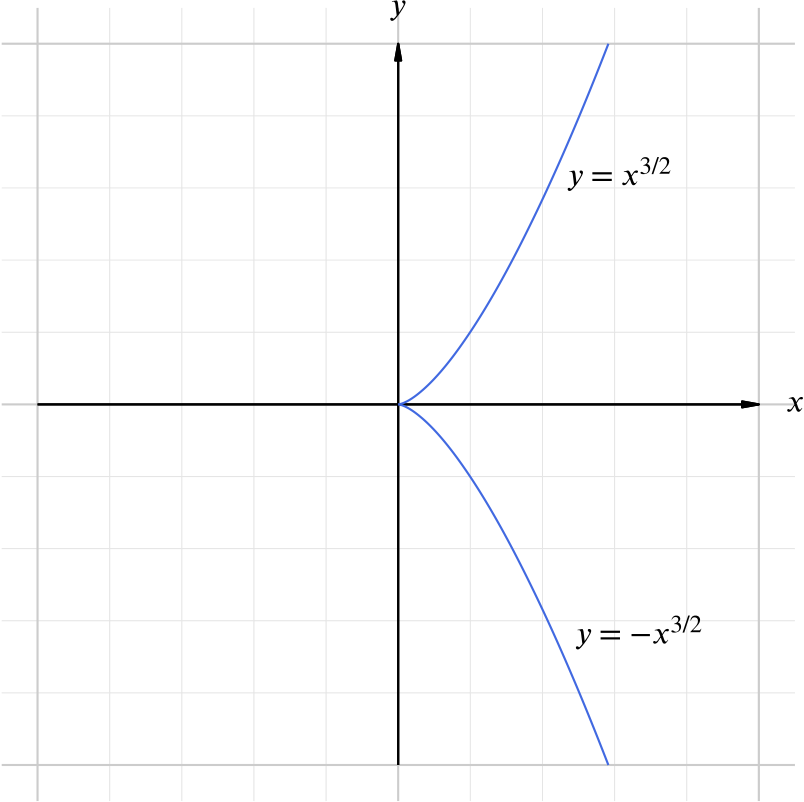
\includegraphics[width=0.5\textwidth]{img/y2x3}
\end{figure}

\begin{proposition}
    Let \(A\) be an integrally closed domain and \(K = \Frac(A)\). Let \(\alpha \in \overline{K}\) (= algebraic closure of \(K\). We can take the closure in any finite extension). We have \(A \subset K \subset \overline{K}\). Consider \(\alpha \in \overline{K}\).

    Then, \(\alpha\) is integral over \(A\) iff the minimal polynomial \(p_\alpha (x) \in K[x]\) of \(\alpha\) over \(K\) 
\end{proposition}

Note that minimal polynomial often depends on base field. For example, \(\sqrt[4]{2}\) has min poly \(x^4 - 2\) over \(\mathbb{Q}\) and \(x^2 - \sqrt{2}\) over \(\mathbb{Q} (\sqrt{2})\) 

\begin{proof}
    \(\impliedby\) by definition.

    \(\implies \): we have \(\alpha \) is integral.

    So, we have monic \(g(x)\in A[x]\) which is monic and \(g(\alpha) = 0\).

    Can we write \(g(x) = h(x) p_\alpha(x)\) in \(K[x]\)?

    Note that every root \(\beta\in \overline{K}\) of \(p_\alpha(x)\) is a root of \(g\). So, all roots of \(p_\alpha(x)\) are integral over \(A\).
    
    Note that coefficients of \(p_\alpha(x)\) are generated by the roots of the polynomial. The coefficients are the elementary symmetric polynomials.

    Thus, coefficients of \(p_\alpha\) lie in \(B \coloneqq \{ \alpha \in \overline{K} \mid \alpha \text{ is integral over } A \} \) 
    
    They also lie in \(K\)

    So, the coefficients are integral over \(A\) and in \(K\), hence in \(A\).

\end{proof}

Proposition 1.5 can be used to find \(\mathcal{O}_K\) for quadratic extension, \([K : \mathbb{Q} ] = 2\) (HW)

\subsection*{Preliminaries from the theory of fields}


In the following \(L / K\) will be a finite extension of fields.

\(L / K\) is called \underline{simple} if \(\exists \theta \in L\) such that \(L = K(\theta)\) 

\(L / K\) is called \underline{separable} if every \(\alpha \in L\) has a separable minimal polynomial over \(K\) [separable polynomial meaning no double roots in any extension field.]

For example, in \(K = \mathbb{F}_p(t)\) and \(L   = K(\sqrt[p]{t})\). Then \(p_{\sqrt[p]{t}}(x) = x^p - t = (x - \sqrt[p]{t})^p\) so not separable

\begin{theorem}
    [Theorem of the Primitive Element]
    
    If \(L / K\) is a finite separable extension, it is simple. 
\end{theorem}

\begin{definition}
    The \underline{trace} \(\operatorname{Tr}_{L / K} : L \to K \) and norm \(\N_{L / K}: L \to K\) are defined by:
    
        \(\Tr_{L / K}(x) = \Tr(T_x)\) 
        
        \(N_{L / L}(x) = \det (T_x)\) 

    Where \(T_x : L \to L\) is defined by \(T_x(y) = xy\) considered as an element of \(\End_K(L)\) 
\end{definition}

If \(n = [L : K]\) and \(f_x(t) = \det (t \operatorname{id}_L - T_x) = t^n + \alpha_1 t^{n-1} + \dots \) 

Then \(Tr _{L / K}(x) = -\alpha\) and \(N_{L / K}(x) = (-1)^n a_n\) 

Since \(T_{x+y} = T_x + T_y\) and \(T_{xy} = T_x \cdot T_y\) we have:

\(\Tr_{L / K}(x + y) = \Tr(T_{x+y}) = \Tr(T_x + T_y) = \Tr(T_x)+\Tr(T_y)=\Tr_{L / K}(x)+\Tr_{L / K}(y)\) 

\(N_{L / K}(xy) = \det(T_{xy})=\det(T_x T_y)=\det(T_x)\det(T_y)=N_{L / K}(x) N_{L / K}(y)\).

So, \(\Tr_{L / K}:L \to K\) is a homomorphism of vector spaces and \(N_{L / K}:L^\times \to K^\times\) is a homomorphism of the (product) group.

\begin{definition}
    Fix an algebraic closure \(\overline{L} \) of \(L\). A \underline{\(K\)-embedding} of \(L\) into \(E\) is a field homomorphism \(\sigma : L \to \overline{L}\) so tat \(\sigma(x) = x\) for all \(x\in K\).

    In other words, \(\sigma : L \to \overline{L} \) so that \(\sigma\) is \(K\)-linear.

    \(\Sigma (L / K)\) is the set of all such embeddings.
\end{definition}

Suppose \(L / K\) is simple and \(L = K(\theta)\). Let \(p_\theta (t)\in K[t]\) be the minimal polynomial of \(\theta\) over \(K\).

Then, the map from \(\Sigma (L / K)\) to the set of roots of the minimal polynomial \(\alpha \in \overline{L} \mid p_\theta (\alpha) = 0\) given by \(\sigma \mapsto \sigma(\theta)\) is a bijection.

In particular if \(L / K\) separable, then: \(\vert \Sigma (L / K) \vert = \deg(p_{\theta})=[L : K]\).

\begin{lemma}
Let \(L \) be finite and \(K \subset M \subset L\) an intermediate field. Then the restriction map \(\operatorname{res} : \Sigma (L / K) \to \Sigma (M / K)\) given by \(\operatorname{res}(\sigma) = \sigma \mid_M\)  is surjective.

Now suppose that \(\Sigma (M / K) \to \Sigma (L / K)\), given by \(\tau \mapsto \tilde{\tau}\), is any right inverse of \(\operatorname{res}\) [meaning, \(\tilde{\tau } \mid _M = \tau\)]. Then, for each \(\tau \in \Sigma(M / K)\), the map \(\operatorname{res}^{-1} (\tau) : \Sigma (L / K) \to \Sigma (\tilde{\tau}(L) / \tilde{\tau}(M))\) given by \(\sigma \mapsto [\tilde{\tau}(y) \mapsto \sigma(y)]\)  is bijective.\footnote{Here we consider \(\overline{L}\) as an algebraic closure of \(\tilde{\tau}(L) \subset L\).}
\end{lemma}

\begin{proof}
    Lorenz, \emph{Algebra}, Volume 1, chapter 7, section 1, Lemma.
\end{proof}

\begin{proposition}
    Let \(L / K\) be finite separable and \(x\in L\). Then,
    
    \begin{enumerate}[label=\roman*)]
        \item  \(f_x(t) = \det (t \id_L - T_x) = \prod_{\sigma \in \Sigma (L / K)}^{}(t - \sigma(x)) \)
        
        \item \(\Tr_{L / K}(x) = \Sigma_{\sigma \in \Sigma (L / K)} \sigma(x)\) 
        
        \item \(N_{L / K}(x) = \prod_{\sigma \in \Sigma (L / K)} \sigma (x)\) 
        
        \item If \(K \subset M \subset L\), then \(\Tr_{L / K} = \Tr_{M / K} \circ \Tr_{L / M}\) and \(N_{L / K} = N_{M / K} \circ N_{L / M}\). 

    \end{enumerate}  

\end{proposition}

\begin{proof}
    Neukirch, ch I, 2.6 and 2.7
\end{proof}

\begin{definition}
    Let \(L /K\) be finite separable extension and \(\alpha_1, \dots , \alpha_n\) be basis of \(L\) as a \(K\) vector space.

    Then the discriminant of \(\alpha_1, \dots ,\alpha_n\) is defined by:

    \(d(\alpha_1, \dots , \alpha_n) = \det(\sigma_i(\alpha_j))^2\) where \(\Sigma (L / K) = \{ \sigma_1, \dots , \sigma_n \} \) 
\end{definition}

\underline{Remark:} \(d(\alpha_1, \dots , \alpha_n)\) does not depend on the ordering of \(\alpha_1, \dots , \alpha_n\) and not on the chosen ordering of the elements in \(\Sigma(L / K)\) 

We now show that the \(d(\alpha_1, \dots , \alpha_n)\) is in \(K\). Let \(S\) be the matrix.

\[d(\alpha_1, \dots , \alpha_n) = \det(S)^2 = \det(S)\det(S^T) = \det (S^T S)\]

\[
    =\det \left[ \left[ \sum_{k} \sigma_k(\alpha_i)\sigma_k(\alpha_j) \right]_{ij}\right] = \det \left[ \left[ \sum_{k} \sigma_k(\alpha_i\alpha_j) \right]_{ij}\right]
\]
 
\[
    = \det \left[ (\Tr_{L / K} (\alpha_i \alpha_j) )_{ij} \right] 
\]

Since the trace is in \(K\), we see that the determinant must also be in \(K\).

\section*{Tuesday, 9/3/2024}

\subsection*{The Discriminant}

Let \(L / K\) be a finite separable field extension, and \((\alpha_1, \dots , \alpha_n)\) a basis of \(L / K\). Then,

\[
    d(\alpha_1, \dots , \alpha_n) = \det[(\sigma_i(\alpha_j))_{1 \le i,j \le n}]^2
\]

Where \(\Sigma(L / K) = \{ \sigma_1, \dots , \sigma_n \}\). Note that this is independent of order.

We have seen,

\[
    d(\alpha_1, \dots , \alpha_n) = \det \left[ (\Tr_{L / K}(\alpha_i \alpha_j))_{i j} \right] \in K
\]

In fact this is an alternate definition.

\begin{proposition}

    Let \(L / K\) be any (possibly inseparable) finite field extension. Then the \(K\)-bilinear form

    \[
        L \times L \to K, (x,y) = \Tr_{L / K}(xy)
    \]

is non-degenrate if and only if \(L / K\) is separable. In this case, \(d(\alpha_1, \dots , \alpha_n) \neq 0\) for any \underline{basis} \((\alpha_1, \dots , \alpha _n)\) of \(L / K\).

\end{proposition}


\begin{proof}
    Sketch \(\impliedby\): Let \(L = K(\theta)\). It can be proven [HW2] that
    
    \[
        d(1, \theta , \theta ^2, \dots , \theta^{n-1}) = \prod_{1 \leq i \neq j \leq n}^{} (\theta_i - \theta_j)^2
    \]
    
    where \(\theta_i\) are the conjugates of \(\theta\) in \(\overline{L}\).

    This finishes the proof.
\end{proof}

\underline{General Setting}: Let \(A\) be an integral domain, \(K = \Frac(A)\). Suppose \(L / K\) is a finite separable extension.

\(B \coloneqq \) integral closure of \(A\) in \(L\). Let \(C\) be the integral closure of \(A\) in \(\overline{L}\).

Assume in the following that \(A\) is integrally closed.

\underline{Observation}: If \(x\in B \subset C\) then \(\forall \sigma \in \Sigma (L / K), \sigma(x)\in C\).

Therefore, \(\Tr_{L / K}(x) = \Sigma_{\sigma \in \Sigma (L / K)} \sigma(x) \in C \cap K = A\) [since \(A\) is integrally closed.]

Similarly, \(N_{L / K}(x) = \prod_{\sigma \in \Sigma (L / K)}^{} \sigma (x) \in C\cap K = A\).

So, the norm and trace of elements of \(B\) are contained in \(A\). 

\underline{Remark}: If \(x\in B\), then \(x\in B^{\times} \iff N_{L / K} (x)\in A^\times\) 

\begin{proof}
    Suppose \(xy = 1\) for some \(y\in B \implies N_{L / K}(xy) = 1 \implies N_{L / K}(x) N_{L / K}(y) = 1\).

    For the other direction, \(N_{L / K}(x) = x \underbrace{\prod_{\sigma \neq \id}^{} \sigma(x)}_{b} = xb\). Note that \(b \in C \cap L = B\). 

    Since the norm is a unit, there exists \(a\in A \subset B\) such that \(axb = 1\). Therefore, \(x(ab) = 1 \implies x\in B^\times\).

\end{proof}

\begin{lemma}
    Let \((\alpha_1, \dots , \alpha_n)\) be a basis of \(L / K\) such that \(\alpha_i \in B\). Then,

    \[
        d(\alpha_1, \dots , \alpha_n) B \subset A \alpha_1 + \dots + A \alpha_n
    \]
\end{lemma}

\begin{proof}
    By 1.9, we may assume \(L / K\) is separable. Write an arbitrary element \(\alpha \in B\) as \(\alpha = a_1 \alpha _1 + \dots + a_n \alpha_n\) with \(a_i \in K\).

    Then, \(\Tr(\alpha_i \alpha) = \sum_{j=1}^{n} \Tr(\alpha_i \alpha_j)a_j = \begin{bmatrix}
        \Tr(\alpha_i \alpha_1) & \cdots &  \Tr(\alpha_i \alpha_n)  \\
    \end{bmatrix}\begin{bmatrix}
        a_1 \\
        \vdots \\
        a_n \\
   \end{bmatrix}\). Therefore,

   \[
    \begin{bmatrix}
        \Tr(\alpha_1 \alpha) \\
        \vdots \\
        \Tr(\alpha_n \alpha) \\
      \end{bmatrix}=\underbrace{[\overbrace{\Tr(\alpha_i \alpha_j)}^{\in A}]_{1 \leq i, j \leq n}}_{S} \begin{bmatrix}
             a_1 \\
             \vdots \\
             a_n \\
        \end{bmatrix}
   \]

    Multiplying on the left by \(S^{\ast}\) [the adjugate matrix of \(S\)],

    \[S^{\ast} S \begin{bmatrix}
         a_1 \\
         \vdots \\
         a_n \\
    \end{bmatrix} = S^{\ast} \begin{bmatrix}
         \Tr(\alpha_1 \alpha) \\
         \vdots \\
         \Tr(\alpha_n \alpha) \\
    \end{bmatrix}
    \] 

    \[\underbrace{\det(S)}_{d(\alpha_1, \dots , \alpha_n)} \begin{bmatrix}
        a_1 \\
        \vdots \\
        a_n \\
   \end{bmatrix} = \underbrace{S^{\ast}}_{\text{all entries are in } A} \begin{bmatrix}
        \Tr(\alpha_1 \alpha) \\
        \vdots \\
        \Tr(\alpha_n \alpha)\\
   \end{bmatrix} \in A^n
   \]

   Therefore, \(d(\alpha_1, \dots , \alpha_n)\alpha  = (\underbrace{d(\alpha_1, \cdots , \alpha_n) a_1}_{\in A}) \alpha_1 + \cdots + (\underbrace{d(\alpha_1, \cdots , \alpha_n) a_1}_{\in A})\alpha_n\) 

\end{proof}

\underline{Example}: Let \(K = \mathbb{Q} , L = \mathbb{Q}(\sqrt{5}), \alpha_1 = 1, \alpha_2 = \sqrt{5}\)

Then \(A = \mathbb{Z} , B = \mathbb{Z} \left[ \frac{1+\sqrt{5}}{2} \right] \) and \(d(1, \sqrt{5}) = \det \begin{bmatrix}
    1 &  \sqrt{5} \\
    1 &  -\sqrt{5} \\
\end{bmatrix} = 20\) 

Then, \(20 \cdot \mathbb{Z} \left[ \frac{1+\sqrt{5}}{2} \right] \subset \mathbb{Z} + \mathbb{Z} \sqrt{5} = \mathbb{Z} [\sqrt{5}] \) 

\underline{Remarks}:

\begin{enumerate}[label=\arabic*)] 

\item \(\forall \alpha \in L, \exists a \in A \setminus \{ 0 \}\) such that \(a \alpha \in B\).

\begin{proof}
    Suppose minimal polynomial of \(\alpha \) over \(K\) is \(p_\alpha (x) = x^d + a_1 x^{d-1} + \dots + a_d \in K[x] \implies \exists a \in A \setminus \{ 0 \} \) such that \(a a_i \in A, 1 \leq i \leq d\).

    Thus, \((ax)^d + \underbrace{a_1 a}_{\in A}(ax)^{d-1} + \cdots + \underbrace{(a^d a_d)}_{\in A}\).

    Thus, \(a \alpha\) is integral. Therefore, \(a \alpha \in B\)
\end{proof}

    \item \(\operatorname{span}_K(B) = L \)
    \item \(\Frac(B) = L\)  

\end{enumerate}

\begin{definition}
    An \(n\)-tuple \((\omega_1, \cdots, \omega_n)\in B^n\) is called an \underline{integral basis} of \(B\) over \(A\) if \(B = \bigoplus_{i=1}^n A \omega_i\)
\end{definition}

\underline{Remark}: If \((\omega_1, \dots , \omega_n)\) is an integral basis of \(B\) over \(A\), then it is a basis of \(L / K\) and hence \(n = [L : K]\).

Note that integral basis is \underline{not guaranteed} to exist.

\begin{proposition}
    If \(L / K\) is finite separable and \(A\) is a PID, then every finitely generated \(B\)-submodule \(M \neq 0\) of \(L\) is a free \(A\)-module of rank \([L : K]\).

    In particular, \underline{\(B\) has an integral basis over \(A\).} [Apply the proposition to \(M = B\)].
\end{proposition}

\begin{proof}
    Write \(M = \sum_{i=1}^{s} B \alpha_i\) with \(\alpha_i \in L^\times\). By the remark 1 above, we can find \(a \in A \setminus \{ 0 \} \) such that \(a \alpha_i \in B\) for \(1 \leq i \leq s\).

    Therefore, \(a \cdot M \subset B\). Since \(\underset{ax \leftarrow x}{aM \cong M} \) [as \(A\)-module], we may assume \(M \subset B\). 
    
    Therefore, \(\alpha_1 B = \underset{\neq 0}{B \alpha_1} \subset M \subset B\). (1)

    \underline{Fact} (from M502): Let \(A\) be a PID. Then every submodule \(N\) of a finitely generated free \(A\)-module \(F\) is free, and \(\rank_A(N) \leq \rank_A(F)\).

    Applying the fact to (1), it suffices to show that \(B\) is free of rank \(n\) over \(A\).

    Choose a basis \((\alpha_1, \cdots, \alpha_n)\) of \(L / K\) with all \(\alpha_i \in B\).
    
    By 1.10, \(d(\alpha_1, \dots , \alpha_n) B \underset{(2)}{\subset} A \alpha_1 + \cdots + A \alpha_n \underset{(3)}{\subset} B\) 

    Since \((\alpha_1, \cdots, \alpha_n)\) is a basis of \(L / K\), \(A \alpha_1 + \cdots + A \alpha_n\) is finitely generated free \(A\)-module of rank \(n\).
    
    (2) and fact together imply that \(d(\alpha_1, \cdots, \alpha_n) B\) is free of \(\rank \leq n\) over \(A\), and it is nonzero by 1.9.

    But \(B \to d(\alpha_1, \cdots, \alpha_n)B\), \(x \mapsto d(\alpha_1, \cdots, \alpha_n)x\), is an isomorphism of \(A\)-modules.
    
    (3) and fact together imply that \(B\) has rank \(\geq n\). 

    Therefore, \(\rank_A(B) = n\).

\end{proof}

\underline{Remark}: If \(L = K(\alpha)\) and \(p(x) = p_\alpha(x) \in K[x]\) is the minimal polynomial of \(\alpha\) over \(K\).

Let \(\alpha = \alpha_1, \cdots, \alpha_n\) be the roots of \(p_\alpha\) in \(\overline{L}\), counted with multiplicity.

Then, \(d(1, \alpha, \alpha^2, \cdots, \alpha^{n-1}) = \prod_{i < j}^{} (\alpha_i - \alpha_j)^2 = \operatorname{disc}(p_\alpha(x))\)

Recall that \(\operatorname{disc}(p) = \operatorname{resultant}(p, p^{\prime}) \).

\begin{definition}
    Let \(K\) be a number field and \(n = [K : \mathbb{Q}]\).

    \begin{enumerate}[label=\arabic*)]
        \item If \(0 \neq I \subseteq K\) is a finitely generated \(\mathcal{O}_K\)-module and \((\alpha_1, \cdots, \alpha_n)\) a basis of \(I\) as a \(\mathbb{Z}\)-module (exists by 1.11), then \(d(I) \coloneqq d(\alpha_1, \cdots, \alpha_n)\) is called the \underline{discriminant} of \(I\).
        \item \(d_K = d(\mathcal{O}_K)\) is called \underline{the discriminant of \(K\)}.
    \end{enumerate} 

\end{definition}

\underline{Remarks}:

\begin{enumerate}[label=\arabic*)]
    \item \(\mathbb{Z}\) is a PID \(\overset{1.11}{\implies}\) every \(I\) as in \((1)\) is indeed free of rank \(n = [K : \mathbb{Q}]\) over \(\mathbb{Z}\).
    \item \(d(I)\) doesn't depend on the choice of a basis. If \((\beta_1, \cdots, \beta_n)\) is another basis \(I\) over \(\mathbb{Z}\), then we can find a matrix \(M \in M_n(\mathbb{Z})\) such that \(M \begin{bmatrix}
         \alpha_1 \\
         \vdots \\
         \alpha_n \\
    \end{bmatrix} = \begin{bmatrix}
         \beta_1 \\
         \vdots \\
         \beta_1 \\
    \end{bmatrix}\). Note that \(M\)  must be invertible in \(M_n(\mathbb{Z})\) since we can also express the elements of the first basis as linear combination of the elements of the second basis with integral coefficients. Therefore, \(\det(M) \in \{ \pm 1 \}\).

    Therefore, \(\det(\beta_1, \cdots, \beta_n) = \det(M)^2 d(\alpha_1, \cdots, \alpha_n) = d(\alpha_1, \cdots, \alpha_n)\).
\end{enumerate}

\section*{Thursday, 9/5/2024}

\underline{Example}: \(K = \mathbb{Q} (i) \implies \mathcal{O}_K = \mathbb{Z}  + \mathbb{Z} i \implies d_K = \det \begin{bmatrix}
    1 &  i \\
    1 &  -i \\
\end{bmatrix}^2 = -4\).

Note: \(K = \mathbb{Q} (\sqrt{d_K})\). If \([K : \mathbb{Q}] = 2\) then \(K = \mathbb{Q}(\sqrt{d_K} )\) [Exercise]

\begin{proposition}
    Let \(0 \neq I \subset J\) be finitely generated \(\mathcal{O}_K\)-submodules of \(K\). Then,
    
    \[
        d(I) = [J : I]^2 d(J)
    \]
\end{proposition}

\begin{proof}
    Let \(I = \mathbb{Z} \alpha_1 \oplus \cdots \oplus \mathbb{Z} \alpha_n\) and \(J = \mathbb{Z} \beta_1 \oplus \cdots \oplus \mathbb{Z} \beta _n\). Then, there exists \(M \subset M_n(\mathbb{Z})\) such that \(M \begin{bmatrix}
         \beta_1 \\
         \vdots \\
         \beta_n \\
    \end{bmatrix} = \begin{bmatrix}
         \alpha_1 \\
         \vdots \\
         \alpha _n \\
    \end{bmatrix}\). 
    
    Then, \(d(I) = d(\alpha_1, \cdots , \alpha_n) = \det(M)^2 d(\beta_1, \cdots , \beta_n) = \det(M)^2 d(J)\). 
    
    To finish the proof, note that \(J / I \cong \mathbb{Z}^n / M(\mathbb{Z}^n) \cong \mathbb{Z}/(m_1) \oplus \cdots \oplus \mathbb{Z}/(m_n) \implies \vert m_1 \cdots m_n \vert = \vert \det(M) \vert = [J : I]\).

\end{proof}

\begin{corollary}
    If \(0 \neq I \subset \mathcal{O}_K\) is an ideal and \(d(I)\) is square-free, then \(I = \mathcal{O}_K\). If \(\theta \in \mathcal{O}_K\) and \(K = \mathbb{Q}(\theta)\), then \(d(1, \theta , \theta^2, \cdots , \theta^{n-1})\) is square-free, then \(\mathbb{Z}[\theta] =  \mathcal{O}_K\).  
\end{corollary}

\begin{proof}
    \(d(I)\) is square free.
    
    \(1.12 \implies d(I) = [\mathcal{O}_K : I]^2 d(\mathcal{O}_K)\), which is only possible when \([\mathcal{O}_K : I] = 1\).
    
    Suppose \(\mathcal{O}_K = \mathbb{Z} \alpha_1 \oplus \cdots \oplus \mathbb{Z} \alpha_n\) and \(M \in M_n(\mathbb{Z})\) such that \(M \begin{bmatrix}
         \alpha_1 \\
         \vdots \\
         \alpha_n \\
    \end{bmatrix} = \begin{bmatrix}
         1 \\
         \vdots \\
         \theta^{n-1} \\
    \end{bmatrix}\). 

    It follows that \(d(1, \theta , \cdots , \theta^{n-1}) = \det(M)^2 d(\alpha_1, \cdots , \alpha_n)\), implying \(\det(M)^2 = 1\implies \det(M) = \pm 1\). 

    Therefore \(\begin{bmatrix}
         \alpha_1 \\
         \vdots \\
         \alpha_n \\
    \end{bmatrix} = M ^{-1} \begin{bmatrix}
         1 \\
         \vdots \\
         \theta^{n-1} \\
    \end{bmatrix} \implies \mathbb{Z}[\theta] = \mathcal{O}_K\). 
\end{proof}


\chapter{Ideals}

Suppose \(K\) is a number field, and \(\mathcal{O} = \mathcal{O}_K\).

\begin{definition}
    An element \(\alpha \in \mathcal{O} \setminus \{ 0 \} \) is called \underline{irreducible} if \(\alpha\) is not a unit \([\alpha \notin \mathcal{O} ^\times]\) and whenever \(\alpha = \beta \gamma\) with \(\beta , \gamma \in \mathcal{O}\) then either \(\beta \in \mathcal{O} ^\times \) or \(\gamma \in \mathcal{O} ^\times \) 
\end{definition}

This is not the same as the definition of a prime element. In general, irreducible elements may not be prime elements (which are those non-zero elements which generate prime ideals).

\underline{Observation}: Every \(0 \neq \alpha \in \mathcal{O}  \setminus \mathcal{O} ^\times\) can be expressed as a product of irreducible elements.

\begin{proof}
    If \(\alpha\) is irreducible, there's nothing to do.

    If it is not irreducible, then \(\alpha = \beta \gamma\) with \(\beta, \gamma\) both non-units.

    Using the remark before 1.10, \(\vert N_{K / \mathbb{Q}}(\beta) \vert > 1\) and \(\vert N_{K / \mathbb{Q}}(\gamma) \vert > 1\).

    Moreover, \(\vert N_{K / \mathbb{Q}}(\alpha) \vert > \vert N_{K / \mathbb{Q}}(\beta) \vert, \vert N_{K / \mathbb{Q}(\gamma)} \vert\). 

    By applying \underline{strong induction} on \(\vert N_{K / \mathbb{Q}}(\alpha) \vert\), we see that \(\beta \) and \(\gamma\) can be written as products of irreducibles. Thus, \(\alpha\) can be written as a product of irreducibles.  
\end{proof}

\textbf{Example}: \(K = \mathbb{Q} (\sqrt{-5}), \mathcal{O}_K = \mathbb{Z} [\sqrt{-5}]\). Here,

\[
    21 = 3 \cdot 7 = (1 + 2 \sqrt{-5})(1 - 2 \sqrt{-5})
\]

HW2: \(3, 7, 1 + 2 \sqrt{-5}, 1 - 2 \sqrt{-5}\) are all irreducibles and are pairwise non-associates.

\(\implies\) factorization into irreducibles is \underline{not} unique.

[This is equivalent to the fact that not every irreducible element is a prime element.]

\underline{Conclusion}: \(\mathcal{O}_K\) is not a UFD in general!

\begin{theorem}
    The ring \(\mathcal{O}_K\) is noetherian, integrally closed and every non-zero prime ideal is maximal [\(\iff \) Krull dimension of \(\mathcal{O}_K\) is \(1\)].
\end{theorem}

\begin{proof}
    \underline{\(\mathcal{O}_K\) is noetherian}: if \(0 \neq I \subset \mathcal{O}_K\) is an ideal \(\overset{1.11}{\implies} I\) is a finitely generated as a \(\mathbb{Z}\)-module \(\implies I\) is finitely generated as an \(\mathcal{O}_K\)-module.
    
    \underline{\(\mathcal{O}_K\) is integrally closed}: remark after 1.4.

    \underline{Non-zero prime ideals are maximal}: Suppose \(0 \neq P \subset \mathcal{O}_K\) is a non-zero prime ideal.
    
    \(\overset{1.12}{\implies} [\mathcal{O}_K : P]\) is finite. In fact, \(d(P) = [\mathcal{O}_K : P]^2 d(\mathcal{O}_K)\).
    
    Hence, \(\mathcal{O}_K / P\) is a finite integral domain. But finite integral domains are fields.

    Thus, \(\mathcal{O}_K / P\) is a field, and thus \(P\) is maximal.

\end{proof}

This gives us the inspiration to define Dedekind domain.

\begin{definition}
    An integral domain \(A\) is called \underline{Dedekind domain} if:

    \begin{enumerate}[label=\arabic*)]
        \item \(A\) is noetherian.
        \item \(A\) is integrally closed.
        \item Every non-zero prime ideal \(P\) of \(A\) is maximal. 
    \end{enumerate} 
\end{definition}

By Theorem 2.1, \(\mathcal{O}_K\) is a \underline{Dedekind domain}.

Moreover, we have:

\begin{enumerate}[label=\arabic*)]
    \item \(k[x]\) when \(k\) is a field is a Dedekind domain.
    \item \(\mathbb{C}[x,y] / (y^2 - x^3)\) is \underline{not} a Dedekind domain. It fails the integrally closed condition, as we saw earlier. 
\end{enumerate} 

From now on, \(\mathcal{O}\) denotes a Dedekind domain.

\begin{definition}
    \(\operatorname{Id}(\mathcal{O}) =\) set of ideals of \(\mathcal{O}\).

    \(\operatorname{Id^\times}(\mathcal{O}) = \operatorname{Id}(\mathcal{O} ) \setminus \{ (0) \}\).

    \(\operatorname{Max}(\mathcal{O}) =\) set of maximal ideals of \(\mathcal{O} \). 
\end{definition}

\begin{lemma}
    \(\forall I \in \operatorname{Id^\times }(\mathcal{O}) \), there exists primes \(P_1, \cdots , P_r \in \operatorname{Max}(\mathcal{O}) \) such that \(P_1 \cdots P_r \subset I\).
\end{lemma}

\begin{proof}
    Suppose \(X = \{ J \in \operatorname{Id^\times }(\mathcal{O}) \mid J \text{ does not contain a product of maximal ideals} \} \)
    
    Note that \(X\) does not contain \(\mathcal{O} = (1)\) since it \(X\) contains all the prime ideals.

    \underline{Goal}: We want to show that \(X = \varnothing\). Suppose \(X\) is non-empty. Since \(\mathcal{O}\) is noetherian, we cannot have infinite ascending chains.

    Using the fact that \(X\) is partially ordered by \(\subset\), \(X\) contains maximal elements. Let \(I \in X\) be a maximal element.

    Since \(I\in X\), \(I\) is not a prime. Which means, we can find \(x,y\notin I\) such that \(xy\in I\).
    
    Set \(I_1 \coloneqq (x)+I\) and \(I_2 \coloneqq (y)+I\).

    Then, \(I_1\) and \(I_2\) contain \(I\). Since \(I\) is maximal, \(I_1, I_2\notin X\).

    This means we can find \(P_1, \cdots , P_m\) and \(Q_1, \cdots, Q_{m^{\prime}}\) such that \(\prod_{i=1}^m P_i \subset I_1\) and \(\prod_{j=1}^{m^{\prime}} Q_j \subset I_2\).

    Then, \(\prod_i P_i \prod_j Q_j \subset I_1 I_2 = ((x)+I)((y)+I)\), since \(xy\in I\) we have \(I_1 I_2 \subset I\). 

\end{proof}

\begin{lemma}
    Suppose \(P \in \operatorname{Max}(\mathcal{O})\) and \(P ^{-1} = \left\{ x \in \underset{=\Frac(\mathcal{O})}{K} \mid xP \subset \mathcal{O} \right\} \) [this is an \(\mathcal{O}\)-submodule of \(K\), containing \(\mathcal{O}\)]
    
    Then, \(\forall I \in \operatorname{Id^\times}(\mathcal{O}), I P ^{-1} \supsetneq I\).
\end{lemma}

\begin{proof}
    \underline{Step 1}: We sow \(P ^{-1} \supsetneq \mathcal{O}\). Suppose \(c \in P \setminus \{ 0 \} \).

    \(2.2 \implies \exists P_1, \cdots , P_r \in \operatorname{Max}(\mathcal{O}) \) such that \(P_1 \cdots P_r \subset (c) = c \cdot \mathcal{O} \subset P\)

    Assume that \(r\) is minimal with this property.

    Recall that, if ideal product \(IJ \subset P\) then \(I \subset P\) or \(J \subset P\).

    Therefore, there exists \(i\) such that \(P_i \subset P\). Since \(P_i\) is also a maximal ideal, \(P_i = P\).

    This means the chain of subsets are all equalities. By reordering the prime ideals, we may assume \(i = 1\).

    Since \(r\) is minimal, \(P_2 P_3 \cdots P_r \not \subset (c)\).
    
    This implies there exists \(b \in P_2, \cdots , P_r \setminus (c)\) such that \(\underset{\in K}{\dfrac{b}{c}} \notin \mathcal{O} \). However,

    \[
        \frac{b}{c} \cdot P = \frac{b}{c} \subset P_1 \subset \frac{1}{c} P_2 \cdots P_r P_1 \subset \frac{1}{c}(c) = \mathcal{O}
    \]

    Therefore, \(\frac{b}{c} \in P ^{-1} \setminus \mathcal{O} \implies P ^{-1} \supsetneq \mathcal{O}\).

    \underline{Step 2}: We'll show: \(I P ^{-1} \supsetneq I\) where \(I \neq (0)\).

    Write \(I = \sum_{i=1}^{m} \mathcal{O} \alpha_i\) where \(\alpha_i \neq 0\).

    Suppose \(I P ^{-1} = I \implies \) if \(x \in P ^{-1}\), then \(x \alpha _i = \sum_{j=1}^{m} a_{ij} \alpha_j\).

    Set \(A \coloneqq \left[ x \partial _{ij} - a_{ij} \right] _{1 \leq i, j \leq m}\). Then, \(A \begin{bmatrix}
         \alpha_1 \\
         \vdots \\
         \alpha _m \\
    \end{bmatrix} = \begin{bmatrix}
         0 \\
         \vdots \\
         0 \\
    \end{bmatrix}\). Multiplying on the left by \(A^{\ast}\) we see  that,

    \[
        \det (A) \begin{bmatrix}
             \alpha_1 \\
             \vdots \\
             \alpha_m \\
        \end{bmatrix} = \begin{bmatrix}
             0 \\
             \vdots \\
             0 \\
        \end{bmatrix} \implies \forall i, \det(A) \alpha_i = 0 \implies \det (A) = 0
    \]

    Since \(\det (A)\) is a monic polynomial, we deduce that \(x\) is integral over \(\mathcal{O}\), which means \(x\in \mathcal{O}\). Therefore, \(P ^{-1} \subset \mathcal{O}\). This is a contradiction.

    Therefore, \(I P ^{-1} \supsetneq I\).
\end{proof}

\begin{theorem}[Unique Factorization in Dedekind Domain]
    Every \(I \in \operatorname{Id^\times}(\mathcal{O}) \) can be written as:

    \[
        I = P_1 P_2 \cdots P_r
    \]

    with \(P_1, \cdots , P_r \in \operatorname{Max}(\mathcal{O})\), and this factorization is unique upto ordering. 
\end{theorem}

\section*{Tuesday, 9/10/2024}

\begin{proof}

    Step 1, Existence:

    Let \(X = \{ J \in \operatorname{Id^\times }(\mathcal{O}) \mid J \text{ does not have a factorization into prime ideals} \} \). We want to show that \(X = \varnothing\).

    Assume \(X \neq \varnothing\). \(\mathcal{O}\) is a dedekind domain, and thus it is noetherian. Therefore, \(X\) has a maximal element \(I\).

    \(I \neq \mathcal{O}\) [since \(\mathcal{O} \notin X\)].

    Thus, there is a maximal ideal \(P\) containing \(I\).

    Since \(I\in X\), \(I \neq P\). Therefore, \(P\supsetneq I\).

    By lemma 2.3, \(I P ^{-1} \supsetneq I\).

    Again, by lemma \(2.3\), \(P ^{-1} P \supsetneq P\), \(P ^{-1} P\) is an ideal \(\subsetneq \mathcal{O}\). Therefore, by the maximality of \(P\), we see that \(P ^{-1} P = \mathcal{O}\).
    
    Now, suppose \(\mathcal{O} = I P ^{-1} \). Multiplying both sides by \(P = I P ^{-1} P = I\), which is a contradiction.
    
    Thus, \(I \subsetneq I P ^{-1} \subsetneq \mathcal{O}\).

    Now, since \(I\) is a maximal element of \(X\), \(I P ^{-1} \notin X\).

    Thus, we can find maximal ideals \(P_1, \cdots , P_r\) so that \(I P ^{-1} = P_1 \cdots P_r\).

    Multiplying both sides by \(P\), we see that,

    \(I = I P ^{-1} P = P_1 \cdots P_r P \) which is a contradiction.

    Thus, \(X\) must be empty. This shows existence.

    Uniqueness: HW.

\end{proof}

\begin{theorem}
    [Chinese Remainder Theorem]

    Let \(I_1, \cdots , I_r\) be ideals of a ring \(R\) which are pairwise co-prime [i.e. \(I_i + I_j = R \quad \forall i \neq j\)]. Then,
    
    \begin{enumerate}[label=\roman*)]
        \item \(I_1 \cdots I_r = \bigcap_{j=1}^{r} I_j\)  
        \item The canonical map \(R / \bigcap_{j=1}^{r} I_j \to \prod_{j=1}^{r} R / I_j\) sending \(a + \bigcap_{j=1}^{r} I_j \mapsto (a + I_j)^r_{j=1}\) is a ring isomorphism.
    \end{enumerate} 

\end{theorem}

\begin{proof}
    Neukirch 3.6, Atiyah-MacDonald
\end{proof}

\begin{definition}
    Let \(\mathcal{O}\) be a Dedekind domain, and \(K = \Frac(\mathcal{O})\). Then, a \underline{fractional ideal} of \(K\) is a non-zero finitely generated \(\mathcal{O}\)-submodule of \(K\).
    
    For any \(a \in K^\times\), we call \(a \cdot \mathcal{O}\) a \underline{principal fractional ideal}.
    
    The non-zero ideals of \(\mathcal{O}\) are called \underline{integral ideals}.

    We denote by \(\mathcal{J}_K\) the set of fractional ideals of \(K\), and by \(\mathcal{P}_K\) the set of principal fractional ideals.

\end{definition}

\begin{example}
    \(\frac{1}{2}\mathbb{Z}\) is a fractional ideal for \(\mathcal{O} = \mathbb{Z}\). 
\end{example}

\underline{Observation}: Let \(I \subset K\) be a non-zero \(\mathcal{O}\)-submodule.

Then \(I\) is fractional of \(K \iff \exists c\in \mathcal{O} \setminus \{ 0 \}\) such that \(c \cdot I \subset \mathcal{O}\).

\begin{proof}
    If it is a fractional ideal of \(K\), it is finitely generated as an \(\mathcal{O} \)-module. Suppose it is generated by \( \frac{a_1}{s_1}, \dots, \frac{a_r}{s_r}   \) for nonzero \(s_1, \cdots , s_r \in \mathcal{O}\). We can set \(c = s_1 \cdots s_r\) which gives us \(c \cdot I = 0\).

    For the other direction, suppose \(c \cdot I \subsetneq \mathcal{O}\). Since \(\mathcal{O}\) is noetherian, it is finitely generated as an \(\mathcal{O}\)-module.

    Therefore, \(I = \frac{1}{c}(cI)\) is also finitely generated as an \(\mathcal{O}\)-module. Thus, \(I\) satisfies all the conditions of being a fractional ideal, and thus is a fractional ideal by definition. 

\end{proof}

\begin{proposition}
    [Definition of Ideal Group] The fractional ideals of \(K\) form an abelian group w.r.t.\ multiplication, which is called the \underline{ideal group} of \(K\).
    
    The identity element is \((1) = \mathcal{O}\).

    Inverse is given by \(I ^{-1} = \{ x \in K \mid xI \subsetneq \mathcal{O} \} \) 
\end{proposition}

\begin{proof}
    First we prove that the product of two fractional ideals are fractional ideals.

    \(I, J \subset \mathcal{J}_K \implies cI \subset \mathcal{O}, dJ \subset \mathcal{O}\). Therefore, \((cd)IJ = (cI)(dJ) \subset \mathcal{O}\). Therefore, \(IJ \subset \mathcal{J}_K\).

    Commutatitivty and associativity follows from \(\mathcal{O}\) itself being a commutative ring.

    We need to prove the existence of inverses. Idea: \((P_1 \cdots P_r) ^{-1} = P_1 ^{-1} \cdots P_r ^{-1}\) 

    Given \(I \subset \mathcal{J}_K, \exists c \in \mathcal{O} \setminus \{ 0 \} \) such that \(cI \subseteq \mathcal{O} \).

    We can factor \(cI\) into primes. Thus, \(cI = P_1 \cdots P_r\).

    For any \(J \in \mathcal{J}_K\), we define \(\overline{J} = \{ x \in K \mid xJ \subseteq \mathcal{O} \} \).

    Note that, if \(d\in J \setminus \{ 0 \}\), we have \(d \overline{J} \subseteq \mathcal{O}\).

    Furthermore, \(d \overline{J} \) is finitely generatd implies \(\overline{J} = \frac{1}{d} = \frac{1}{d}(d \overline{J})\) is finitely generated as a \(\mathcal{O}\)-module. 
    
    Thus, \(\overline{J} \in \mathcal{J}_K\).

    Going back to \(I\), we see that \((c) \overline{P_1} \cdots \overline{P_r} I = \overline{P_1} \cdots \overline{P_r} (cI) = (\overline{P}_1 P_1) \cdots (\overline{P_r} P_r) = \mathcal{O} \cdots \mathcal{O} = \mathcal{O}\).  

    Thus, \(\forall J \in \mathcal{J}_K, \exists J ^{-1} \in \mathcal{J}_K\) such that \(J ^{-1} \cdot J = J \cdot J ^{-1} = \mathcal{O}\).

\end{proof}

\begin{corollary}
    Every \(I \in \mathcal{J}_K\) has a factorization:

    \[
        I = P_1 ^ {e_1} \cdots P_r^{e_r}
    \]

    where \(P_1, \cdots , P_r\) are pairwise distinct prime/maximal ideals and \(e_1, \cdots , e_r\) are uniquely determiend integers.

    As usual, if \(e < 0\) then \(J^e \coloneqq (J ^{-1} )^{-e}\) for any \(J \in \mathcal{J}_K\).

\end{corollary}

\begin{proof}
    Choose \(c \in \mathcal{O} \setminus \{ 0 \} \) so that \(cI \subset \mathcal{O} \implies cI = P_1^{a_1}\cdots P_r^{a_r}\) with \(a_i \geq 0\).

    Also write \(c \mathcal{O} = P_1^{b_1}\cdots P_r^{b_r}\) with \(b_i \geq 0\).

    Exponent of \(0\) are allowed to make sure the primes are the same.

    Therefore, \(I = (c)^{-1} (cI) = P_1^{a_1 - b_1} \cdots P_r^{a_r - b_r}\) 

    Uniqueness is HW.

\end{proof}

Note that, in the group of (fractional) ideals, the principal ideals form a subgroup.

\begin{definition}
    The \underline{ideal class group} of \(K\) is defined as \(\mathcal{J}_K / \mathcal{P}_K\) and denoted by \(\Cl_K\). We call \(h_K = \vert \Cl_K \vert \) the \underline{class number} of \(K\).
\end{definition}

We have the exact sequences:

\[
    1 \to \mathcal{P}_K \to \mathcal{J}_K \to \Cl_K \to 1
\]

\[
    1 \to \mathcal{O} ^\times \to \underset{c}{K^\times} \underset{\mapsto}{\to} \underset{c \mathcal{O}}{\mathcal{P}_K} \to 1
\]

\underline{Remark}: \(\mathcal{O}\) is a PID \(\iff \Cl_K = \{ 1 \}\)

\begin{proof}
    Suppose \(I\) is a fractional ideal. Then, \(cI\) is an ideal for some \(c\). Since \(\mathcal{O}\) is a PID, we see that \(cI\) is a principal ideal, so \(cI = (d)\). Therefore, \(I = \frac{d}{c} \mathcal{O}\). Thus, \(\mathcal{J}_K = \mathcal{P}_K \implies \Cl_K = \{ 1 \}\).

    For the other direction, suppose \(\Cl_K = \{ 1 \}\). Then, \(\mathcal{J}_K = \mathcal{P}_K\). Given \(I \in \operatorname{Id^\times }(\mathcal{O})\) there exists \(c\in K^\times\) such that \(I = c \mathcal{O}\). Since \(c\in I\) we see that \(I\) is a principal ideal. 
\end{proof}

Note that \(\Cl_K\) being trivial is also equivalent to \(\mathcal{O}\) being a UFD.

The main results of the first part of the course are: if \(K\) is a number field,

\begin{itemize}
    \item The finiteness of the class number
    \item Dirichlet's Theorem on Units.
    
    \(\mathcal{O}_K^\times \cong \mathbb{Z}^{r + s - 1} \oplus \{ \text{roots of unity in \(K\)}  \} \)
    
    Where \(r\) is the number of real embeddings 
    
    \(r = \vert \{ K \hookrightarrow \mathbb{R} \}  \vert \).
    
    And \(2s\) is the number of complex embeddings which do not factor through \(\mathbb{R} \)
    
    \(2s = \vert \{ K \underset{\mathbb{Q}}{\hookrightarrow} \mathbb{C} \text{ does not factor through } \mathbb{R} \}  \vert \).
\end{itemize} 

\subsection*{Decomposition of primes in \(\mathcal{O}_K\)}

c.f. Neuker, ch I

Here, \(K =\) number field, \(\mathcal{O} = \mathcal{O}_K, n = [K : \mathbb{Q}]\).

\begin{definition}
    Given a prime number \(p \in \mathbb{Z}_{> 0}\) we write \(p \cdot \mathcal{O}_K = P_1^{e_1} \cdots P_r^{e_r} \quad (\ast)\) with pairwise distinct maximal ideals $P_i$. \(p\) is called:

    \begin{enumerate}[label=\roman*)]
        \item \underline{unramified} (in \(K\)) if \(e_1 = \cdots = e_r = 1\).
        \item \underline{ramified} (in \(K\)) if \(\exists 1 \leq i \leq r : e_i > 1\).
        \item \underline{completely split} (\underline{totally split}, \underline{totally demomposed}) if it is unramified and \(r = n\).
        \item \underline{inert} if \(r = 1, e_1 = 1\).
    \end{enumerate} 
\end{definition}

\begin{example}
    Suppose \(K = \mathbb{Q} (i)\), then \(\mathcal{O}_K = \mathbb{Z} [i]\) and \(2 \cdot \mathbb{Z} [i] = (1+i)^2\) so \(2\) ramified.

    If \(p \equiv 1 \pmod 4\) then \(p \mathbb{Z} [i] = P_1 P_2\) with \(P_1 \neq P_2\) maximal ideals, so \(p\) is completely split [and also unramified].
    
    If \(p \equiv 3 \pmod 4\) then \(p \mathbb{Z} [i]\) is a maximal ideal, therefore \(p\) is inert.

\end{example}

\underline{Fundamental Questions}: Given \(K\), how can we characterize

\[
    \operatorname{Spl}_K = \{ p \in \mathbb{Z} _{>0} \text{ is prime} \mid p \text{ is totally split in } K \} \,?
\]

In \(\mathbb{Q} (i)\) we have a rule: \(p \equiv 1 \pmod 4\) if and only if \(p\) is totally split. For quadratic extensions we have similar rules. More generally, if the Galois closure of $K$ over $\mathbb{Q}$ has an abelian Galois group over $\mathbb{Q}$, then $\operatorname{Spl}_K$ can be described using congruence conditions.

If the Galois group of (the normal closure of) $K$ over $\mathbb{Q}$ is not abelian, one can sometimes use modular forms or Maass forms to describe $\operatorname{Spl}_K$. In general, the \emph{Langlands Program} predicts that one can use automorphic representations to describe $\operatorname{Spl}_K$.

\section*{Thursday, 9/12/2024}

Recall that,

\[
    \operatorname{Spl}_K = \{ p \in \mathbb{Z} _{>0} \mid p \text{ is totally split in } K \}
\]

\begin{example}
    \(\operatorname{Spl}_{\mathbb{Q}(\sqrt{-3})} = \{ p \text{ prime } \mid p\equiv 1 \pmod 3 \} \)

    \(\operatorname{Spl}_{\mathbb{Q} (\sqrt[3]{2})} = \{ p \text{ prime } \mid \exists x,y\in \mathbb{Z} \times \mathbb{Z} : p = x^2 +27y^2 \}  \) 

\end{example}

We can write:

\[
    p \mathcal{O} _K = P_1^{e_1} \cdots P_r^{e_r} \text{ with pairwise distinct } P_i\in \operatorname{Max} (\mathcal{O} _K), e_i > 0 \quad(\ast)
\]

\underline{Question}: How does one find a decomposition \((\ast)\)?

\begin{definition}[Conductor]
    Let \(\theta \in \mathcal{O} = \mathcal{O}_K\) such that \(K = \mathbb{Q} (\theta)\).Then,

    \[
        C = \{ \alpha \in \mathcal{O} \mid \alpha \mathcal{O} \subset \mathbb{Z} [\theta] \} 
    \]

    \(C\) is called the \underline{conductor} of \(\mathbb{Z} [\theta]\).

    This is an ideal in \(\mathcal{O}\). 

    \underline{Note}: 1.10 implies, \(d(1, \theta , \cdots , \theta^{n-1})\cdot \mathcal{O} \subset \mathbb{Z} + \mathbb{Z} \theta + \cdots + \mathbb{Z} \theta ^{n-1} = \mathbb{Z} [\theta]\) where \(n = [K : \mathbb{Q}]\). Thus, \(d(1, \theta , \cdots , \theta^{n-1}) \in C \implies C \neq 0\)  

    \underline{Note}: \(Q\in \operatorname{Max} (\mathbb{Z} [\theta])\) so that \(Q\) is not invertible in \(\mathbb{Z}[\theta] \iff C \subset Q\). \(C\) is the largest ideal of \(\mathcal{O}_K\) such that: if \(Q \in \operatorname{Max}(\mathbb{Z}[\theta])\) is not invertible in \(\mathbb{Z} [\theta] \iff C \subset Q\).   

\end{definition}

\begin{definition}[Norm of an Ideal]
    If \(I \in \operatorname{Id} ^\times (\mathcal{O})\) then \(N(I) = [\mathcal{O} : I]\) is called the \underline{norm} of \(I\) [finite by 1.12].
\end{definition}

\begin{lemma}
    For \(I, J \in \operatorname{Id} ^\times (\mathcal{O})\), \(N(I \cdot J) = N(I)N(J)\).
\end{lemma}

\begin{proof}
    Write \(I = P_1^{e_1} \cdots P_r^{e_r}\) by 2.4. By 2.5, \(\mathcal{O} / I \cong \prod_{i=1}^{r} \mathcal{O} / P_i^{e_i} \implies N(I) = \prod_{i=1}^r N(P_i^{e_i})\). 

    So, the norm is multiplicative in distinct prime factors.

    It suffices to show that for non-zero prime ideals \(P\), we have \(N(P^e) = N(P)^e\).
    
    We consider the following filtration of \(P^e\):

    \[
        P^e \subset P^{e-1} \subset P^{e-2} \subset \cdots \subset P \subset \mathcal{O}
    \]

    \[
        \implies \vert \mathcal{O} / P^e \vert = \prod_{i=0}^{e-1} \vert P^i / P^{i+1} \vert
    \]

    With \(P^0 = \mathcal{O}\).

    \underline{Claim}: Since \(\mathcal{O} / P\) is a vector space, \(P^i / P^{i+1}\) is a vector space. Then, \(\dim_{\mathcal{O} / P} P^i / P^{i+1}  = 1\)
    
    \underline{Proof of Claim}: Homework 4.
    
    From the claims, we deduce that \(N(P^e)=N(P)^e\). 
\end{proof}

\begin{theorem}
    [Dedekind] Let \(\theta \in \mathcal{O}_K\) be such that \(K = \mathbb{Q} (\theta)\) and \(\mu_\theta(x) \in \mathbb{Z} [x]\) be the minimal polynomial of \(\theta\) over \(\mathbb{Q}\).

    Let \(p\) be a prime such that \(p \cdot \mathcal{O} + C = \mathcal{O}\) where \(C\) is the conductor of \(\mathbb{Z}[\theta]\). [\(p\) is relatively prime to the conductor. This is always true for \(\mathbb{Z}[\theta] = \mathcal{O}\)] [This condition only excludes at most finitely many primes].

    Let \(\mu \mod p \in \mathbb{Z} [x] / p \mathbb{Z}[x] = \mathbb{F}_p(x)\). Since \(\mathbb{F}_p[x]\) is a UFD, we can write,
    
    \[
        \overline{\mu} = \overline{\mu}_1^{e_1} \cdots \overline{\mu}_r^{e_r}
    \]

    where \(\overline{\mu}_1, \cdots, \overline{\mu }_r\) are pairwise distinct monic irreduible polynomials over \(\mathbb{F}_p[x]\). 

    Let \(\mu_i(x) \in \mathbb{Z} [x]\) be any polynomial such that \(\mu_i \mod p = \overline{\mu}_i\)

    Then, \(P_i \coloneqq (p, \mu_i(\theta)) \in \operatorname{Max} (\mathcal{O})\) for \(1 \leq i \leq r\) and \(p\mathcal{O} =P_e^{e_1}\cdots P_r^{e_r}\)  
\end{theorem}

Note that, \(p\mathcal{O} + C = \mathcal{O}\) implies \(\mathbb{Z} [\theta] / p \mathbb{Z} [\theta] \cong \mathcal{O} / p \mathcal{O}\).

\begin{proof}
    \underline{Claim}: \(p\mathbb{Z} + (C\cap \mathbb{Z}) = \mathbb{Z}\)
    
    \underline{Proof of Claim}: If not, since \(p\mathbb{Z}\) is a maximal ideal, we have \(C\cap \mathbb{Z} \subseteq p\mathbb{Z}\). Also, \(C\cap \mathbb{Z}\) is non-empty since the discriminant is in it.

    Therefore, \(\mathbb{Z} / (C\cap\mathbb{Z}) \rightarrowtail \mathbb{Z} / p\mathbb{Z}\) [surjectve]
    
    Thus, \(p \mid N(\mathbb{Z} \cap C) = [\mathbb{Z} : C\cap\mathbb{Z}]\).

    On the other hand, \(\mathbb{Z} / (\mathbb{Z} \cap C) \hookrightarrow \mathcal{O} / C\). 

    Therefore, \(p \mid [\mathcal{O} : C] = N(C)\). 

    Write \(C = Q_1^{f_1}\cdots Q_s^{f_s}\) prime factorization. 

    2.8 \(\implies N(C) = \prod_{j=1}^{s} N(Q_j)^{f_j} \implies \exists 1 \leq j \leq s : P \mid N(Q_j) = \vert \mathcal{O} / Q_j \vert\).

    Therefore, \(p = \operatorname{char} (\mathcal{O} / Q_j) \implies p\cdot 1_{\mathcal{O} / \mathcal{O}_j} = 0 \implies p\in Q_j\).

    But then, since \(C \subset Q_j\), \(p\cdot \mathcal{O} + C \subset p \cdot \mathcal{O} + Q_j \subset Q_j\), which is a contradiction. This proves the claim.

    Therefore, \(p\mathbb{Z} + (\mathbb{Z} \cap C) = \mathbb{Z}\).

    Recall that \(C = \{ \alpha \in \mathcal{O} \mid \alpha \cdot \mathcal{O} \subset \mathbb{Z} [\theta] \} \subset \mathbb{Z} [\theta]\).

    \[
        \implies \mathcal{O}  = p\mathcal{O} + C \subseteq p \mathcal{O}  + \mathbb{Z} [\theta] \subseteq \mathcal{O}
    \]

    \(\implies \mathcal{O} = p \mathcal{O} + \mathbb{Z} [\theta]\) 
    
    \(\implies \mathbb{Z} [\theta] / p \mathbb{Z} [\theta] \rightarrowtail \mathcal{O} / p 
    \mathcal{O}\) is a surjection (1). Furthermore,

    \(\mathbb{Z} [\theta] \cap p \mathcal{O} \underset{\text{claim}}{=} (\mathbb{Z} [\theta]\cap p \mathcal{O}) (p\mathbb{Z} +(\mathbb{Z} \cap C)) \subseteq p \mathbb{Z} [\theta] + p \mathcal{O} (\mathbb{Z} \cap C) \subseteq p\mathbb{Z} [\theta] + p \mathcal{O} \cdot C \subseteq p\mathbb{Z}[\theta]\) 

    \underline{Upshot}: \(\mathbb{Z} [\theta] / p \mathbb{Z} [\theta] \overset{\cong}{\to} \mathcal{O} / p\mathcal{O}\) is an isomorphism. (2)

    This gives us an isomorphism of rings:

    \[
        \mathbb{F}_p[x] / (\overline{\mu} (x)) \overset{\cong}{\to} \mathbb{Z}[\theta] / p \mathbb{Z} [\theta] \overset{\cong}{\to} \mathcal{O} / p\mathcal{O}
    \]

    First isomorphism is given by \(f(x) + (\overline{\mu }(x)) \mapsto f(\theta) + p \mathbb{Z} [\theta]\) 

    Let \(\varphi\) be the map from \(\mathbb{F}_p[x]/(\overline{\mu } (x)) \to \mathcal{O} / p \mathcal{P}\). 


    Chinese remainder theorem gives us:

    \[
        \mathbb{F}_p[x]/(\overline{\mu} (x)) = \prod_{i=1}^r \mathbb{F}_p[x] / (\overline{\mu_i}(x)^{e_i} )
    \]

    Then, the prime ideals of \(\mathcal{O} / p \mathcal{P}\) are precisely \(\varphi(\overline{\mu}_i(x)) = \underset{=\overline{\mathcal{P}}_i}{\mu_i(\theta)+p \mathcal{O}} \in \mathcal{O}/ p \mathcal{O} \leftarrowtail \mathcal{O}\).

    Therefore, prime ideals of \(\mathcal{O}\) containing \(\mathcal{O}\) are precisely the ideals \(\mathcal{P}_i \coloneqq (\mu_i(\theta),p)\). Also, 

    \[
        \bigcap_{i=1}^{r} (\overline{\mu_i}(x)^{e_i}) \overset{CRT}{=} (0_{\mathbb{F}_p[x] / (\overline{\mu}(x))})
    \]

    \[
        \implies \bigcap_{i=1}^{r} \overline{\mathcal{P}_i^{e_i}} = (0_{\mathcal{O} / p \mathcal{O}}) \implies \prod_{i=1}^{r} \mathcal{P}_i^{e_i} \subset p \mathcal{O}
    \]

    If \(n = [K : \mathbb{Q}]\) then \(p^n = \underset{[\underset{\oplus_1^n \mathbb{Z} \alpha_i}{\mathcal{O}} : \underset{\oplus_1^n p \mathbb{Z} \alpha_i}{p \mathcal{O} ]}}N(p\mathcal{O}) \leq \prod_{i=1}^r (P_i^{e_i}) = \prod N(P_i)^{e_i} = \prod [\mathcal{O} : P_i]^{e_i} = p^{\deg(\mu)} = p^n\). 
    
    Therefore, \(p^n = \prod_{i=1}^{r} N(P_i^{e_i}) \implies \boxed{\prod_{i=1}^r P_i^{e_i} = p \mathcal{O}}\) 

\end{proof}

\begin{example}
    Let \(K = \mathbb{Q} (\sqrt{D})\) for \(D \in \mathbb{Z} \setminus \{ 0,1 \}, D\) square-free, \underline{and} \(D \equiv 1\pmod 4 \underset{HW}{\implies} \mathcal{O}_K = \mathbb{Z} \left[ \frac{1+\sqrt{D}}{2} \right]  \). 

    Recall that minimal polyonomial of \(\frac{1+\sqrt{D}}{2}\) is given by:

    \[
        \mu (x) = x^2 - x- \frac{1-D}{4}
    \]

    If \(p \neq 2\) then \(\mu(x) \pmod p\) is equivalent to the factorization of \(4 \mu(x) \pmod p\).
    
    \[
        4 \mu(x) =4x^2 -4x + (1-D) = (2x-1)^2 - D
    \]

    It splits into two distinct factors of degree \(1\) if and only if \(D\) is a quadratic residue \(\pmod p\).

    This gives us the cases:

    \(p \mid D\) then \(y^2 - D \equiv y^2 \pmod p\) and therefore \(p\) \underline{ramifies} in \(K\) 

    \(D\) is not a square \(\pmod p\) then \(y^2 - D\) is irreducible \(\pmod p\) and therefore \(p\) is inert in \(K\).

    \(D\) is a square \(\pmod p\) then \(y^2 - D\) has two distinct roots and therefore \(p\) is totally split in \(K\).

    For which primes \(p\) is \(D\) a square?

    Answer: We use \underline{Quadratic Reciprocity}. This gives us,

    \[
        \operatorname{Spl}_{\mathbb{Q} (\sqrt{D} )} \overset{.}{=} \left\{ p \text{ prime } \mid  p\nmid D \text{ and the Jacobi symbol } \left( \frac{p}{D} \right) = 1\right\} 
    \]

    \(\overset{.}{=}\) means ``up to at most finitely many exceptions''.

    If \(D=q\) a prime number, then we have,

    \[
        \left( \frac{q}{p} \right) = \left( \frac{p}{l} \right) (-1)^{\frac{p-1}{2}\cdot\frac{q-1}{2}}
    \]

    Since in our case \(p \equiv 1 \pmod 4\) we have,

    \[
        \left( \frac{q}{p} \right) = \left( \frac{p}{q} \right) 
    \]

    If \(D = \prod_{i=1}^r q_i\) we have,

    \[
        \left( \frac{p}{D} \right) = \prod_{i=1}^r \left( \frac{p}{q_i} \right) 
    \]

    \underline{Consequence}: There exists finitely many congruence classes \(\overline{a}_1 , ..,\overline{a}_s \in \mathbb{Z} / D\mathbb{Z}\) such that, 

    \[
        p \in \operatorname{Spl}_{K} \iff \exists 1 \leq i \leq s : p \equiv a_i \pmod D
    \]

\end{example}

\section*{Tuesday, 9/17/2024}

\(D \equiv 1\pmod 4, K = \mathbb{Q} (\sqrt{D})\) implies:

\[
    \operatorname{Spl} _K = \left\{ p \text{ prime } \mid p\nmid D \text{ and } \left( \frac{p}{D} \right) = 1 \right\}.
\]

If \(D \equiv 2, 3 \pmod 4\) then there s a similar description of \(\operatorname{Spl} _K\) in terms of congruences mod \(4D\).

\begin{corollary}
    For a number field \(K\) there are only finitely many primes \(p\) which \underline{ramify} in \(K\).
\end{corollary}

\begin{proof}
    Suppose \(K = \mathbb{Q} (\theta)\) so that \(\theta \in \mathcal{O}_K\). Set \(C\) to be the conductor of \(\mathbb{Z}[\theta]\).

    \underline{Note}: Only finitely many primes \(p\) \underline{do not satisfy} \(p \mathcal{O}_K + C = \mathcal{O}_K\). 

    If \(p\) has this property [\(p \mathcal{O} _K + C = \mathcal{O} _K\)] then \(p\) ramifies in \(\mathcal{O}_K\) if and only if the minimal polynomial of \(\theta \): \(\mu_{\theta , \mathbb{Q}}(x) \pmod p\) has prime factors in \(\mathbb{F} _p(x)\) with multiplicity \(> 1\) [by theorem 2.9, Dedekind-Kummer]
    
    \(\iff\) \(\mu _\theta (x) \pmod p\) has multiple roots

    \(\iff \operatorname{disc}(\mu_\theta (x) \pmod p) \in \mathbb{F}_p\) vanishes

    \(\iff\) \(\operatorname{disc} (\mu_\theta)\) is divisible by \(p\). [since discriminant of \(\mu_\theta\) is a polynomial in coefficients]

    Since \(\mu_\theta\) is separable, \(\operatorname{disc} (\mu_\theta) \neq 0\) and so only finitely many primes \(p\) divide \(\operatorname{disc} (\mu_\theta)\). 
\end{proof}

\underline{Consequences of proof of 2.10}: If \(\mathcal{O}_K = \mathbb{Z} [\theta]\) then the primes that ramify in \(K\) are exactly those that divide \(\operatorname{disc}(\mu_\theta) = d(1,\theta , \cdots , \theta^{n-1}) = d_K\).

\begin{example}
    [Splitting primes in cyclotomic fields]

    Suppose \(K = \mathbb{Q} (\zeta _n)\). Then, \(\mathcal{O}_K = \mathbb{Z} [\zeta_n]\). [Will be proved later].

    Minimal polynomial \(\mu_{\zeta_n}(x) = \Phi_n(x) = n\)'th cylotomic polynomial. Fix a prime \(p\). Then,

    \[
        p \in \operatorname{Spl}_K \underset{2.9}{\iff} \Phi_n(x) \pmod p \text{ has } d = \phi(n) \text{ distinct roots in } \mathbb{F}_p \text{ [HW]}
    \]

    \[
        \underset{n\not\equiv 2 \pmod 4}{\iff} x^n - 1 \text{ has \(n\) distinct roots in } \mathbb{F} _p
    \]

    \[
        \iff \mathbb{F}_p^\times \text{ has a subgroup of order } n
    \]

    \[
        \iff n \mid p-1 \iff p \equiv 1\pmod n
    \]

    So, we have the \underline{theorem}:

    If \(n \not\equiv 2 \pmod 4\) then \(\operatorname{Spl}_{\mathbb{Q}(\zeta_n)} = \{ p \text{ prime } \mid p \equiv 1\pmod n \} \) 
\end{example}

\begin{corollary}
    Let \(K,L\) be number fields which are Galois over \(\mathbb{Q}\) and \(M = K . L\) [composite extension, smallest subfield of algebraic extension containing both] Then,

    \[
        \operatorname{Spl}_M \overset{.}{=} \operatorname{Spl}_K \cap \operatorname{Spl}_L
    \]

    [up to finitely many exceptions]
\end{corollary}

\begin{example}
    \[
        \operatorname{Spl}_{\mathbb{Q}(\sqrt{2} + \sqrt{3})} = \operatorname{Spl}_{\mathbb{Q}(\sqrt{2})} \cap \operatorname{Spl}_{\mathbb{Q}(\sqrt{3})}
    \]

    To find \(\operatorname{Spl}_{\mathbb{Q}(\sqrt{2})}\) and \(\operatorname{Spl}_{\mathbb{Q}(\sqrt{3})}\) we need the \underline{Quadratic Reciprocity Law}.
\end{example}

\subsection*{The Quadratic Reciprocity Law (QRL):}

\begin{definition}
    [Legendre Symbol] Let \(p\) be an odd prime. The Legendre symbol is defined by:

    \[
        \left( \frac{\cdot}{p} \right) : \mathbb{F}_p^\times \to \{ 1, -1 \}
    \]

    \[
        \left( \frac{a}{p} \right) = \begin{dcases}
            1, &\text{ if } a = b^2 \text{ for some } b \in \mathbb{F}_p^\times ;\\
            -1, &\text{ if } \text{otherwise}
        \end{dcases}
    \]

    We also define for \(a\in \mathbb{Z} \setminus p\mathbb{Z} : \left( \dfrac{a}{p} \right) \coloneqq \left( \dfrac{a\pmod p}{p} \right) \) 
\end{definition}

Euler proved that,

\[
    \left( \frac{a}{p} \right) \equiv a^{\frac{p-1}{2}} \pmod p
\]

In particular,

\[
    \left( \frac{-1}{p} \right) = (-1)^{\frac{p-1}{2}}
\]

\begin{definition}
    [Gauss Sum] Suppose \(\epsilon_p = \displaystyle\sum_{a\in \mathbb{F} _p ^\times }^{} \left( \dfrac{a}{p} \right) \zeta_p ^ a\) where \(\zeta_p\) is a primitive \(p\)'th root of unity. This is called the \underline{Gauss Sum}.
\end{definition}

Then we have the following lemma:

\begin{lemma}
    \[
        \epsilon_p ^ 2 = \left( \dfrac{-1}{p} \right) p = (-1)^{\frac{p-1}{2}} p
    \]
\end{lemma}

\begin{proof}
    HW 5.
\end{proof}

\underline{Note}: \(\vert \epsilon_p \vert _{\mathbb{C}} = \sqrt{p}\) [by 2.12].

\begin{theorem}
    [Quadratic Reciprocity Law / QRL]

    For two distinct odd primes \(p\) and \(l\) we have:

    \[
        \left( \cfrac{p}{l} \right) \left( \cfrac{l}{p} \right) = (-1)^{\frac{p-1}{2}\cdot \frac{l-1}{2}}
    \]

    Moreover, \(\left( \frac{2}{p} \right) = (-1)^{\frac{p^2 - 1}{8}}\) and \(\left( \frac{-1}{p} \right) = (-1)^{\frac{p-1}{2}}\). 
\end{theorem}

\begin{proof}
    Set \(\zeta = \zeta_p\), and the Gauss sum \(\epsilon = \epsilon _ p\) 

    For all \(x,y \in \mathbb{Z} [\zeta]\) we have:

    \[
        (x+y)^l \equiv x^l + y^l \pmod {l\mathbb{Z}[\zeta]}
    \]

    Therefore, using the fact \(\left( \frac{\cdot}{p} \right) \) is a homomorphism, 

    \[
        \epsilon^l \equiv \sum_{a\neq 0}\left( \frac{a}{l} \right) ^ l \zeta ^{al} = \sum_{a\neq 0} \left( \frac{a}{l} \right) \zeta ^{al} \underset{b = al}{=} \sum_{b \neq 0} \left( \frac{bl^{-1}}{p} \right) \zeta ^ b = \left( \frac{l ^{-1}}{p} \right) \epsilon = \left( \frac{l}{p} \right) \epsilon \pmod{l \mathbb{Z} [\zeta]} \quad (1)
    \]

    \[
        \implies \epsilon ^{l+1} = \epsilon^l \epsilon \overset{(1)}{\equiv} \left( \frac{l}{p} \right) \underbrace{\epsilon \cdot \epsilon}_{\epsilon ^2} \overset{2.2}{=} \left( \frac{l}{p} \right) \left( \frac{-1}{p} \right) p \pmod{l \mathbb{Z} [\zeta]} \quad (2)
    \]

    But also:

    \[
        \epsilon ^{l+1} = (\epsilon^2)^{\frac{l+1}{2}} \overset{2.12}{=} \left( \left( \cfrac{-1}{p} \right) p \right) ^{\frac{l+1}{2}} = \left( \left( \cfrac{-1}{p} \right) p \right) ^{\frac{l-1}{2} + 1} = \left( \cfrac{-1}{p} \right) ^{\frac{l-1}{2}} p^{\frac{l-1}{2}} \left( \cfrac{-1}{p} \right) p
    \]

    \[
        \overset{\text{Euler}}{\equiv} (-1)^{\frac{p-1}{2}\frac{l-1}{2}} \left( \frac{p}{l} \right) \left( \frac{-1}{p} \right) \pmod{l \mathbb{Z}[\zeta]} \quad(3)
    \]

    Combining \(2\) and \(3\) we get:

    \[
        \left( \cfrac{l}{p} \right) \left( \cfrac{-1}{p} \right) p \equiv (-1)^{\frac{p-1}{2}\frac{l-1}{2}} \left( \cfrac{p}{l} \right) \left( \cfrac{-1}{p} \right) p \pmod{l\mathbb{Z}[\zeta]} 
    \]

    Cancelling,

    \[
        \left( \cfrac{l}{p} \right) \equiv (-1)^{\frac{p-1}{2}\frac{q-1}{2}} \left( \cfrac{p}{l} \right) \pmod{l\mathbb{Z}[\zeta]} \overset{l > 2}{\implies } \text{Statement} 
    \]

\end{proof}

\begin{corollary}
    Let \(D \in \mathbb{Z} \setminus \{ 0,1 \} \) be square free and \(K = \mathbb{Q} (\sqrt{D}) \). Let \(d_K\) be the discriminant of \(K\). Then there exists a group homomorphismism:

    \[
        \chi : (\mathbb{Z} / d_k \mathbb{Z})^\times \to \{ -1,1 \} \text{ s.t.} 
    \]

    \[
        \operatorname{Spl}_K = \left\{ p \text{ prime } \mid p\nmid d_K \text{ and } \chi(p \pmod{d_K}) = 1 \right\} 
    \]
\end{corollary}

\chapter{Lattices}

\begin{definition}
    Let \(V\) be an \(n\)-dimensional \(\mathbb{R} \)-vector space. A subgroup \(\Gamma \subset V\) is called a \underline{lattice} if:

    \[
        \Gamma = \mathbb{Z} v_1 + \cdots + \mathbb{Z} v_m
    \]

    where \((v_1, \cdots , v_m)\) is a linearly independent set of vectors. \((v_1, \cdots , v_m)\) is called a \underline{basis} for \(\Gamma\). \(\Gamma\) is called \underline{complete} if \(m = \dim V\). The set

    \[
        \Phi = \left\{ \sum_{i=1}^m x_i v_i \mid \forall 1 \leq i \leq m : x_i \in [0,1)  \right\}
    \]

    is called the \underline{fundamental mesh} associated to the basis \((v_1, \cdots , v_m)\) 
\end{definition}

\begin{example}
    Suppose \(V = \mathbb{C} = \mathbb{R} \cdot 1 \oplus \mathbb{R} i\). Then, \(\mathbb{Z} = \mathbb{Z} + \mathbb{Z} i\) is a lattice.

    \begin{center}
        \includegraphics*[width=0.3\textwidth]{img/2D}
    \end{center}

\end{example}

\begin{proposition}
    A subgroup \(\Gamma\) of \(V\) [a finite dimensional \(\mathbb{R} \)-vector space] is a lattice \(\iff\) it is \underline{discrete} [i.e. \(\exists\) open neighborhood \(U\) of \(0_V\) in \(V\) so that \(U \cap \Gamma = \{ 0 \}\)]  
\end{proposition}

\begin{proof}
    \(\implies\): If it is a lattice, we can write \(\Gamma = \mathbb{Z} v_1 + \cdots \mathbb{Z} v_m\) where \((v_1, \cdots , v_m)\) is part of a basis \((v_1, \cdots , v_n)\) with \(n = \dim_{\mathbb{R}}V\). Then,

    \[
        U = \left\{ \sum_{i=1}^n x_i v_i \mid x_i \in \left( -\frac{1}{2}, \frac{1}{2} \right)   \right\} 
    \]

    is open in \(V\) and \(U \cap \Gamma = \{ 0 \}\). Thus, \(\Gamma\) must be discrete.

    
    \section*{Thursday, 9/19/2024}
    
    \(\impliedby\): Assume \(\Gamma\) is descrete.
    
    \underline{Claim}: \(\Gamma\) is closed.

    \underline{Proof of Claim}: Fix a norm \(\lVert \cdot \rVert \) on \(V\). Assume \(\Gamma\) is not closed.

    Then, for \(v_0 \in V \setminus \Gamma\) we can find a sequence \((\gamma_i)_{i \geq 1}\) in \(\Gamma\)  such that \(\gamma_i \neq \gamma_{i+1}\) and \(\lim_{i \to \infty} \gamma_i = v_0\). 

    Thus, \(0 < \lVert \gamma_{i+1} - \gamma_i \rVert \to 0\) as \(i \to \infty\). 

    Thus, in any neighborhood of \(0\), there are infinitely many distinct elements in \(\Gamma\). Then \(\Gamma\) is not discrete. This is a contradiction.

    Therefore, \(\Gamma\) is closed.

    Now we resume the main proof.

    Set \(U = \operatorname{Span}_\mathbb{R} \Gamma \subset\) and set \(m \coloneqq \dim_\mathbb{R} (U)\) Let \(v_1, \cdots , v_m\) be a basis of \(U\) contained in \(\Gamma\). 

    \(\Phi_0 =\) \underline{fundamental mesh} associated to this basis. 

    Set \(\Gamma_0 \coloneqq \mathbb{Z} v_1 + \cdots + \mathbb{Z} v_m \leq \Gamma\).

    \underline{Claim}: \([\Gamma : \Gamma_0] < \infty\). 

    \underline{Proof of Claim}: Given \(\gamma \in \Gamma\) write \(\gamma = \mu(\gamma) + \gamma_0(\gamma)\) where \(\gamma_0(\gamma) \in \Gamma_0\) and \(\mu(\gamma) \in \Phi_0\).

    Note that $\mu(\gamma) \in \Gamma$. Hence \(S = \{ \mu(\gamma) \mid \gamma \in \Gamma \} \subseteq \Gamma \cap \overline{\Phi}_0\). 

    As $\Gamma$ is closed and $\overline{\Phi_0}$ is compact, \(\Gamma \cap \overline{\Phi_0}\) is closed in a compact set and hence compact. But it is also discrete (as $\Gamma$ is discrete), so it is finite. Therefore, \(S\) must also be finite. 

    Thus, \([\Gamma : \Gamma_0]\) is finite.

    Now, set \(q \coloneqq [\Gamma : \Gamma_0]\).

    Then, \(q \Gamma \subset \gamma_0\). Therefore,

    \[
        \Gamma \subset \frac{1}{q}\Gamma_0 = \mathbb{Z}\left( \frac{1}{q}v_1 \right) \oplus \cdots \oplus \mathbb{Z} \left( \frac{1}{q}v_m \right) 
    \]

    Thus, \(\Gamma\) is contained in a finitely generated abelian group of rank \(m\) which is generated by an $\mathbb R$-linearly independent set of vectors. This implies that \(\Gamma\) itself is generated by an $\mathbb R$-linearly independent set of vectors. 

    Thus \(\Gamma\) is a lattice.

\end{proof}

\begin{proposition}
    [Complete Lattices] A lattice \(\Gamma \subset V\) is \underline{complete} \(\iff\) there exists a bounded [with respect to a fixed but arbitrary norm] set \(M \subset V\) so that \(V = \bigcup_{\gamma \in \Gamma}^{} \gamma +M\). 
\end{proposition}

\begin{proof}
    \(\implies \): If \(\Gamma = \mathbb{Z} v_1 + \cdots + \mathbb{Z} v_n\) is a complete lattice where \((v_1, \cdots , v_n)\) is a basis of \(V\) then we can take for \(M\) the fundamental mesh associated to this basis.

    \(\impliedby\): Fix a norm \(\lVert \cdot \rVert \) in \(V\) and suppose there exists a bounded set \(M\) such that \(V = \bigcup_{\gamma \in \Gamma} (\gamma + M)\). 
    
    Set \(V_0 = \operatorname{Span}_\mathbb{R} (\Gamma)\). For \(v\in V\) and \(j\in \mathbb{Z}_{>0}\) we can choose \(\gamma_j \in \Gamma\) and \(m_j \in M\) such that:

    \[
        j \cdot v \in V = \gamma_j + v_j
    \]

    \[
        \implies v = \underbrace{\frac{1}{j} \gamma_j}_{\in V_0} + \underbrace{\frac{1}{j} m_j}_{\left\lVert \frac{1}{j} m_j \right\rVert \to 0}
    \]

    Then, \(V_0\ni\frac{1}{j} \gamma_j \to v\) and since \(V_0\) is closed in \(V\), \(v\in V_0\). Therefore, \(V_0 = V\) and \(\Gamma\) contains a basis in \(V\). 
\end{proof}

Now suppose \(\langle \cdot , \cdot \rangle : V \times V \to \mathbb{R}\) is an inner product, in which case we have the associated norm:

\[
    \left\lVert v \right\rVert = \sqrt{\langle v, v \rangle } 
\]

Let \(\varepsilon_1, \cdots , \varepsilon_n\) be an ONB [orthonormal basis of \((V, \langle\cdot,\cdot\rangle )\)].

Then, we have an \underline{isometry}

\[
    \iota : (V, \langle \cdot,\cdot \rangle) \to (\mathbb{R}^n, \langle \cdot,\cdot \rangle_{st})
\]

where \(\langle \cdot,\cdot \rangle_{st}\) is the standard inner product. Then,

\[
    \iota \left( \sum_{j=1}^{n} x_j \varepsilon _ j  \right)  = \sum_{j=1}^{n} x_j e_j
\]

Then \(\forall v, w \in V, \langle \iota (v), \iota (w) \rangle_{st} = \langle v, w \rangle \) 

We use \(\iota\) to transfar the Lebesgue measure on \(\mathbb{R}^n\) to \(V\):

\[
    \operatorname{vol}_{\langle , \rangle}(\underbrace{M}_{\subset V}) = \operatorname{vol}_{\operatorname{Leb}} (\iota (M))
\]

Then, the volume of the fundamental w.r.t.\ any orthonormal basis \(\varepsilon_1, \cdots , \varepsilon_n\) mesh is:

\[
    \operatorname{vol}_{\langle , \rangle} (\Phi) = \operatorname{vol}_{\operatorname{Leb}}(\iota(\Phi)) = \operatorname{vol}_{\operatorname{Leb}} \left([0,1)^n\right) = 1
\]

More generally: if \(\underline{v} = (v_1, \cdots , v_n)\) is any basis of \(V\) and \(A\) is the change-of-basis matrix from \(\varepsilon_1 , \cdots , \varepsilon_n\):

\[
    A = \begin{bmatrix}
        a_{11} & \cdots  &  a_{1n} \\
        \vdots & \ddots &  \vdots \\
        a_{n1} & \cdots &  a_{nn} \\
    \end{bmatrix} \iff v_j = \sum_{i=1}^{n} a_{ij} \varepsilon_i
\]

Then, if \(\Phi_{\underline{v}} = \{ \sum x_i v_i \mid x_i\in [0,1) \} \) is the fundamental mesh associated to \(\underline{v}\) we have:

\[
    \boxed{\operatorname{vol}_{\langle , \rangle} = \vert \det A \vert}
\]

\underline{Notation}: If \(\Gamma \subset V\) is a complete lattice with fundamental mesh \(\Phi\) [for some basis of \(\Gamma\)] we set

\[
    \operatorname{vol}_{\langle , \rangle }(\Gamma) \coloneqq \operatorname{vol}_{\langle , \rangle} (\Phi)
\]

and it does not depend on the basis of \(\Gamma\), since the transformation matrix has determinant \(\pm 1\).

\begin{definition}
    [Centrally Symmetric Set, Convex Set]

    A subset \(X \subset V\) is called \underline{centrally symmetric} if \(\forall v\in X\), \(-v \in X\).

    It is called \underline{convex} if \(\forall t\in [0,1]\) and \(\forall v,w\in X\), \(tv + (1-t)w \in X\). Meaning, all points in the \underline{line} between \(v\) and \(w\) are in \(X\).
\end{definition}

\begin{theorem}
    [Lattice Point Theorem] Let \(\Gamma \subset (V, \langle\cdot,\cdot\rangle)\) be a complete lattice and \(X \subset V\) a centrally symmetric and convex measurable subset. Then if \(\operatorname{vol}_{\langle , \rangle}(X) > 2^n \operatorname{vol}(\Gamma)\) where \(n = \operatorname{\dim }_\mathbb{R} (V)\) then,
    
    \[
        X \cap (\Gamma \setminus \{ 0 \}) \neq \varnothing
    \]

    Meaning \(X\) must contain a non-zero lattice point.
\end{theorem}

\begin{example}
    Suppose \(V = \mathbb{R}^2\) with the standard inner product, and \(\Gamma = \mathbb{Z} \oplus \mathbb{Z}\). Take \(X = (-1,1) \times (-1,1)\) So \(\operatorname{vol}(X) = 4\). It does not contain any non-zero lattice point, but that is not a contradiction since \(\operatorname{vol}(X)\) is not strictly bigger than \(4\).

    If we take any convex symmetric set even a little bit bigger, we must have one lattice point.

\end{example}

\begin{proof}
    Suppose \(\gamma_1, \gamma_2 \in \Gamma, \gamma_1 \neq \gamma_2\) and \(\left(\gamma_1 + \frac{1}{2}X \right) \cap \left(\gamma_2 + \frac{1}{2}X\right) \neq \varnothing\) 

    Then, \(\exists x,y\in X\) such that \(\gamma_1 + \frac{1}{2}x = \gamma_2 + \frac{1}{2}y \implies \underbrace{\gamma_1 - \gamma_2}_{\Gamma \setminus \{ 0 \}} = \underbrace{\frac{1}{2}y + \frac{1}{2}(-x)}_{\in X}\) so we're done. 
    
    Now, we use contradiction. Assume that the intersection is empty. Then, for any distinct \(\gamma_1, \gamma_2\in \Gamma\) we must have \(\left( \gamma_1 + \frac{1}{2}X \right) \cap (\gamma_2 + \frac{1}{2}X) = \varnothing\).

    Note that \(\gamma + \frac{1}{2}X\) is measurable. All these are distinct.

    Let \(\Phi\) be a fundamental mesh for \(\Gamma\). Then,

    \[
        \operatorname{vol}(\Phi) \geq \sum_{\gamma \in \Gamma}^{} \operatorname{vol} \left( \left( \gamma + \frac{1}{2} X \right) \cap \Phi \right) 
    \]

    Note that,
    
    \[
        \left( \left( \gamma + \frac{1}{2}X \right) \cap \Phi \right) - \gamma  = (\Phi - \gamma) \cap \frac{1}{2}X
    \]

    Therefore,

    \[
        \operatorname{vol}(\Phi) \geq \sum_{\gamma \in \Gamma}^{} \operatorname{vol} \left( (\Phi - \gamma) \cap \frac{1}{2}X \right) 
    \]

    Furthermore,

    \[
        \operatorname{vol}\left( \frac{1}{2}X \right) = \sum_{\gamma \in \Gamma}^{} \operatorname{vol} \left( \left( \Phi - \gamma \right) \cap \frac{1}{2} X \right) \leq \operatorname{vol}(\Phi) = \operatorname{vol}(\Gamma)
    \]

    \[
        \implies \frac{1}{2^n} \operatorname{vol}(X) \leq \operatorname{vol}(\Gamma)
    \]

    \[
        \implies \operatorname{vol}(X) \leq 2^n \operatorname{vol}(\Gamma)
    \]

    Which contradicts our assumption. So we're done.


\end{proof}

\chapter{Geometry of Numbers}

Goal: We want to find find an embedding \(j : K \hookrightarrow K_{\mathbb{R}}\), a \(\mathbb{Q}\)-linear map where \(K_\mathbb{R}\) is a certain inner product space such that \(\forall I \in \operatorname{Id}^\times (\mathcal{O}_K)\), \(j(I)\) is a complete lattice in \(K_{\mathbb{R}}\). 

\begin{example}
    Suppose \(K = \mathbb{Q}(\sqrt{-1})\). Then \(K_{\mathbb{R}} = \mathbb{C} = \mathbb{R} \oplus \mathbb{R} i\), the embedding \(j\) is the obvious map and \(j(\mathbb{Z}[i]) = \mathbb{Z} \oplus \mathbb{Z} i\) is a complete lattice.
\end{example}

Set \(\Sigma_K = \{ \sigma : K \hookrightarrow \mathbb{C} \mid \sigma  \text{ is a field homomorphism}  \} \).

If \(K = \mathbb{Q} (\theta)\) and \(\mu_{\theta ,\mathbb{Q}}(x) = \prod_{i=1}^n (x - \theta_i)\) where \(\theta_i \in \mathbb{C}\)  then the map \(\Sigma_K \to \{ \theta_1, \cdots , \theta_n \}, \sigma \mapsto \sigma(\theta)\) is bijective.

We call \(\tau \in \Sigma_K\) \underline{real} (respectively \underline{complex}) if \(\tau(K) \subset \mathbb{R}\) (respectively \(\tau(K) \not\subset \mathbb{R}\)).

\section*{Tuesday, 9/24/2024}

Suppose \(\Sigma _K = \{ \tau : K \to \mathbb{C} \} \), \(\begin{dcases}
    \tau \text{ real}, & \iff  \tau \subset \mathbb{R} ;\\
     \tau \text{ complex} , & \iff  \tau(K)\not\subset \mathbb{R}
\end{dcases}\) 

\(K = \mathbb{Q} (\theta)\) and \(\theta_1, \cdots , \theta_n\in\mathbb{C}\) are conjugates of \(\theta\) [=roots of minimal polynomial of \(\theta / \mathbb{Q}\)].

\[
    \Sigma _K \underset{\text{bijection}}{\to} \{ \theta_1, \cdots , \theta_n \}, \tau \to \tau (\theta)
\]

Let \(\rho_1, \cdots , \rho_r : K \hookrightarrow \mathbb{R}\) real embeddings and \(\sigma_1, \cdots , \sigma_s, \overline{\sigma}_1, \cdots , \overline{\sigma}_s : K \implies \mathbb{C}\) complex embeddings [\(\overline{\sigma}(\alpha) = \overline{\sigma(\alpha)}\)]

Then \(n = [K : \mathbb{Q}] = r + 2s\) 

\(K_\mathbb{C} \coloneqq \mathbb{C}^{\Sigma_K} =\) set of maps \(\Sigma_K \to \mathbb{C} = \{ (z_\tau)_{\tau \in \Sigma_K} \mid z_\tau \in \mathbb{C} \} \) 

\(K_\mathbb{R} = \{ (x_1, \cdots , x_r, z_1, \cdots , z_s, \overline{z}_1, \cdots , \overline{z}_s) \in K_\mathbb{C} \mid \forall 1 \leq i \leq r : x_i \in \mathbb{R}, \forall 1 \leq j \leq s : z_j\in \mathbb{C} \} \) 

\(x_i \leftrightarrow x_{e_i}, z_j \leftrightarrow z_{\sigma_j}, \overline{z}_j \leftrightarrow z_{\overline{\sigma}_j}\) 

\(\dim_\mathbb{R} K_\mathbb{R} = r + 2s = n\) 

Let \(\langle , \rangle \) be the restriction of the standard inner product \(\langle , \rangle_{K_\mathbb{C}}\) on \(K_\mathbb{C}\) to \(K_\mathbb{R}\) 

\[
    \langle (z_\tau)_\tau, (w_\tau)_\tau \rangle _{K_\mathbb{C}} = \sum_{\tau \in \Sigma_K} z_\tau \overline{w}_\tau
\]

\[
    \left\langle \begin{bmatrix}
         x_1 \\
         \vdots \\
         x_r \\
         z_1 \\
         \vdots \\
         z_s \\
         \overline{z}_1 \\
         \vdots \\
         \overline{z}_s \\
    \end{bmatrix}, \begin{bmatrix}
         x_1^{\prime}  \\
         \vdots \\
         x_r^{\prime}  \\
         z_1^{\prime}  \\
         \vdots \\
         z_s^{\prime}  \\
         \overline{z}_1^{\prime}  \\
         \vdots \\
         \overline{z}_s^{\prime}  \\
    \end{bmatrix} \right\rangle = \sum_{i=1}^r x_i x_i^{\prime} + \sum_{j=1}^s [z_j \overline{z}_j^{\prime} + \overline{z}_j \overline{\overline{z}_j^{\prime} } ] = \sum_{i=1}^r x_i x_i^{\prime} + \sum_{j=1}^s 2\operatorname{Re}(z_j z_j^{\prime}) \in \mathbb{R} 
\]

Define \(j : K \hookrightarrow K_\mathbb{R}, j(\alpha) = (\tau(\alpha))_{\tau \in \Sigma_K}\in K_\mathbb{R}\) because \(\overline{\sigma }(\alpha) = \overline{\sigma(\alpha)} \)

Define Orthonormal Basis of \(K_\mathbb{R}\) by:

\[
    \varepsilon_k = (0, \cdots , 0, \underbrace{1}_{k\text{'th spot}}, 0, \cdots , 0), 1 \leq j \leq r
\]

\[
    \varepsilon_{r+k} = \frac{1}{\sqrt{2}} (\underbrace{0, \cdots , 0}_{r}, 0, \cdots , \underbrace{1}_{r+k}, 0, \cdots , 0, \underbrace{1}_{r+s+k}, 0,\cdots , 0), 1 \leq k \leq s
\]

\[
    \varepsilon_{r+k} = \frac{1}{\sqrt{2}} (\underbrace{0, \cdots , 0}_{r}, 0, \cdots , \underbrace{i}_{r+k}, 0, \cdots , 0, \underbrace{-i}_{r+s+k}, 0,\cdots , 0), 1 \leq k \leq s
\]

Now, \(\operatorname{vol}_{\langle \cdot,\cdot \rangle} (\text{fundamental mesh associated to } (\varepsilon_1, \cdots , \varepsilon_n)) = 1\) 

\begin{proposition}
    For any ideal \(I\in \operatorname{Id}^\times (\mathcal{O}_K)\) th set \(j(I)\) is a \underline{complete lattice} in \(K_\mathbb{R}\) with \(\operatorname{vol}_{\langle \cdot, \cdot \rangle }(j(I)) = \sqrt{\vert d_K \vert} \cdot N(I) \) 
\end{proposition}

\begin{proof}
    We can write \(I = \mathbb{Z} \alpha_1 \oplus \cdots \oplus \mathbb{Z} \alpha_n\) where \(n = [K : \mathbb{Q}]\). Consider the matrix:

    \[
        A = \begin{bmatrix}
            \vdots & \vdots & \vdots &  \vdots \\
            j(\alpha_1) & j(\alpha_2) & \cdots &  j(\alpha_n) \\
            \vdots & \vdots & \vdots &  \vdots \\
        \end{bmatrix} \in M_n(\mathbb{C})
    \]

    \[
        = \begin{bmatrix}
            \rho_1(\alpha_1) &  &  \rho_1(\alpha_n) \\
            \vdots &  &  \vdots \\
            \rho_r(\alpha_1) &  &  \rho_r(\alpha_n) \\
            \sigma_1(\alpha_1) &  &  \sigma_1(\alpha_n) \\
            \vdots & \cdots &  \vdots \\
            \sigma_s(\alpha_1) &  &  \sigma_s(\alpha_n) \\
            \overline{\sigma}_1(\alpha_1) &  &  \overline{\sigma}_1(\alpha_n) \\
            \vdots &  &  \vdots \\
            \overline{\sigma}_s(\alpha_1) &  &  \overline{\sigma}_s(\alpha_n) \\
        \end{bmatrix}
    \]

    \[
        \implies \det(A)^2 = \det ((\underbrace{\tau_i(\alpha_j)}_{\in \overline{K}}))^2 = d(\alpha_1, \cdots , \alpha_n)
    \]

    Where \(\Sigma_K = \{ \tau_1, \cdots , \tau_n \}\) 

    Proposition 1.12 \(\implies d(\alpha_1, \cdots , \alpha_n) =  d_K  N(I)^2 \quad (1)\).

    Proposition 1.9 \(\implies d(\alpha_1, \cdots , \alpha_n) \neq 0 \implies (j(\alpha_1),\cdots , j(\alpha_n))\) is a linearly independent set of vectors, hence a basis.

    \(\implies j(I) = \mathbb{Z}j(\alpha_1) + \cdots \mathbb{Z} j (\alpha_n)\) is a complete lattice in \(K_\mathbb{R}\).

    \[
        B = \begin{bmatrix}
            \langle j(\alpha_1), \varepsilon_1 \rangle &  &  \langle j(\alpha_n), \varepsilon_1 \rangle  \\
            \vdots & \cdots &  \vdots \\
            \langle j(\alpha_1), \varepsilon_n \rangle  &  &  \langle j(\alpha_n), \varepsilon_n \rangle  \\
        \end{bmatrix} \in M_n(\mathbb{R})
    \]

    \(B\) is the change-of-basis matrix from the orthonormal basis \((\varepsilon_1, \cdots , \varepsilon_n)\) to  \((j(\alpha_1), \cdots , j(\alpha_n))\)
    
    \(\implies \operatorname{vol}_{\langle , \rangle }(j(I)) = \vert \det B \vert \quad (2)\) 
    
    By the definition of \(\langle , \rangle_{K_\mathbb{R}}\) we have: \(B^T B = (\langle j(\alpha_i),j(\alpha_j)\rangle ) = A^T \overline{A} \quad (3)\) 

    Thus, we have

    \[
        \sqrt{\vert d_K \vert} N(I) \overset{1}{=} \vert \det A \vert_\mathbb{C} \overset{3}{=} \vert \det B \vert_\mathbb{C} \overset{2}{=} \operatorname{vol_{\langle , \rangle}} (j(I)) 
    \]

\end{proof}

\begin{lemma}
    The map \(f : K_\mathbb{R} \to \mathbb{R}^n\) given by

    \[
        (\underbrace{x_1, \cdots , x_r}_{\in\mathbb{R}}, \underbrace{z_1, \cdots , z_s}_{\in\mathbb{C}}, \overline{z}_1, \cdots , \overline{z}_s) \mapsto (x_1, \cdots , x_r, \operatorname{Re}(z_1), \cdots , \operatorname{Re}(z_s), \operatorname{Im}(z_1), \cdots , \operatorname{Im}(z_s))
    \]

    Is an isometry of \(\mathbb{R}\)-vector spaces and for any measurable \(X \subset K_\mathbb{R}\) we have:

    \[
        \operatorname{vol}_{\langle \cdot, \cdot \rangle} (X) = 2^s \operatorname{vol}_{\operatorname{Leb}}(f(X))
    \]

\end{lemma}

\begin{proof}
    Let \((\varepsilon_1, \cdots , \varepsilon_n)\) be the orthonormal basis of \(K_\mathbb{R}\) as defined above and 

    \[
        \iota : K_\mathbb{R} \to \mathbb{R}^n, \iota (\nu) = \begin{bmatrix}
             \langle \nu , \varepsilon_1 \rangle \\
             \vdots \\
             \langle \nu , \varepsilon_n \rangle \\
        \end{bmatrix}
    \]

    Then \(\operatorname{vol}_{\langle \cdot,\cdot \rangle}(X) \coloneqq \operatorname{vol}_{\operatorname{Leb}}(\iota(X)) = \operatorname{vol}_{\operatorname{Leb}}((\iota \circ f ^{-1})(f(X))) - \vert \det (\iota \circ f ^{-1}) \vert \operatorname{vol}_{\operatorname{Leb}}(f(X))\) 

    Now,

    \[
        (\iota \circ f ^{-1})(e_i) = \begin{dcases}
            e_i, &\text{ if } 1 \leq i \leq r ;\\
            \sqrt{2} e_i, &\text{ if } r+1 \leq i \leq n
        \end{dcases}
    \]

    This is an exercise.

    Also, \(\vert \det (\iota \circ f ^{-1}) \vert = (\sqrt{2})^{2s} = 2^s\).
\end{proof}

\begin{theorem}
    Let \(I \in \operatorname{Id}^\times (\mathcal{O}_K)\) and let \((c_\tau)_{\tau\in \Sigma_{\tau}}\) be positive real numbers such that \(c_{\overline{\tau}} = c_\tau\) for all \(\tau\in \Sigma_K\). Suppose:
    
    \[
        \prod_{\tau \in \Sigma_K} c_\tau > \left( \frac{2}{\pi} \right)^s \sqrt{\vert d_K \vert} N(I)  
    \]

    Then, \(\exists \alpha \in I \setminus \{ 0 \} \) such that \(\forall \tau  \in \Sigma_K : \vert \tau(\alpha) \vert _{\mathbb{C}} < c_\tau\) 
\end{theorem}

\begin{proof}
    \(X = \{ (z_\tau)_\tau \in K_\mathbb{R} \mid \forall \tau \in \Sigma_K : \vert z_\tau \vert < c_\tau \} \) 

    Note that \(0\in X\) trivially. Also, if \(v\in X\) then \(-v\in X\). Thus \(X\) must be centrally symmetric.

    Also, \(\forall t\in [0,1]\) we have: \(\vert tz_\tau + (1-t)z_\tau^{\prime}  \vert \leq  t \vert z_\tau \vert + (1-t) \vert z_\tau^{\prime}  \vert < c_\tau\) when \(\vert z_\tau \vert , \vert z_\tau^{\prime} \vert < c_\tau\) so \(X\) is conve.

    Now,
    
    \[
        \operatorname{vol}_{\langle , \rangle}(X) \overset{4.2}{=} 2^s \operatorname{vol}_{\operatorname{Leb}}(f(X)) = 2^s \prod_{\tau \text{ real}}(2 c_\tau) \prod_{\substack{\tau \text{ complex} \\ \text{modulo complex conjugation}}}\pi c_\tau^2
    \]

    \[
        = 2^s \cdot 2^r \cdot \pi ^s \prod_{\tau\in \Sigma_K} c_\tau \underset{\text{by assumption}}{>} 2^{r+s} \pi^s \left( \frac{2}{s} \right)^s \sqrt{\vert d_K \vert } N(I) = 2^n \sqrt{\vert d_K \vert} N(I) \overset{4.1}{=} 2^n \operatorname{vol}_{\langle , \rangle} (j(I)) 
    \]

    Lattice Point Theorem implies \(\exists \alpha \in I \setminus \{ 0 \} : j(\alpha)\in X\). Thus it must also satisfies the inequality.
\end{proof}

\begin{lemma}
    For all \(t > 0\) the set \(X_t = \{ (z_\tau)_{\tau} \in K_\mathbb{R} \mid \Sigma_{\tau \in \Sigma_K} \vert z_\tau \vert < t \} \). This set is centrally symmetric and convex, and
    
    \[
        \operatorname{vol}_{\langle , \rangle}(X_t) = 2^n \left( \frac{\pi}{4} \right) ^s \frac{t^n}{n!}
    \]
\end{lemma}

\begin{proof}
    HW5
\end{proof}

The following claim is instrumental in proving the finiteness of the class number.

\begin{theorem}
    \(\forall I \in \operatorname{Id}\dot{\mathcal{O}_K}, \exists \alpha \in I \setminus \{ 0 \} \) such that \(\vert N_{K/\mathbb{Q}}(\alpha)\vert \leq M_K \cdot N(I)\) where
    
    \[
        M_K = \frac{n!}{n^n} \left( \frac{4}{\pi} \right) ^ s \sqrt{\vert d_K \vert}
    \]

    is called the \underline{Minkowski Constant}.
\end{theorem}

\begin{proof}
    Let \(\epsilon > 0\) and set \(t = t_{\epsilon} = n \sqrt[n]{M_K N(I) + \epsilon}\)
    
    Then, applying Lemma 4.4 we see that:

    \[
        \operatorname{vol}_{\langle , \rangle} (X_t) \overset{4.4}{=} 2^n \left( \frac{\pi}{4} \right)^ s \frac{t^n}{n!} = 2^n \left( \frac{\pi}{4} \right)^s \frac{n^n}{n!} (M_K N(I) + \epsilon)
    \]

    \[
        > 2^n \left( \frac{\pi}{4} \right)^s \frac{n^n}{n!} \frac{n!}{n^n} \left( \frac{4}{\pi} \right)^s \sqrt{\vert d_K \vert} N(I) \overset{4.1}{=} 2^n \operatorname{vol}_{\langle , \rangle}(j(I))
    \]

    Lattice Point Theorem \(\implies \exists \alpha \in I \setminus \{ 0 \} : j(\alpha) \in X_t\) therefore \(\sum_{} \vert \tau (\alpha) \vert < t\) 

    Using the AM-GM inequality,

    \[
        \sqrt[n]{\prod_{i=1}^n c_i} \leq \frac{1}{n} \sum_{i=1}^n c_i 
    \]

    \[
        \implies \vert N(\alpha) \vert = \prod_\tau \vert \tau(\alpha) \vert \leq \frac{t^n}{n!} = M_K N(I) + \epsilon 
    \]

    Choose \(\epsilon\) to be small enough so that \(\lfloor M_K N(I)+ \epsilon \rfloor = \lfloor M_K N(I) \rfloor\) 

    Thus, we have \(\vert N_{K / \mathbb{Q}}(\alpha) \vert \leq M_K N(I)\).
\end{proof}

\chapter{The Class Number}


\section*{Thursday, 9/26/2024}

Suppose \(K\) is a number field, \(\mathcal{O} = \mathcal{O}_K\) and \(n = [K:\mathbb{Q}]\). Suppose \(\mathcal{J}_K\) is the group of fractional ideals.

Suppose \(I \in \mathcal{J}_K\). Choose \(\alpha \in \mathcal{O} \setminus \{ 0 \} \) such that \(\alpha I \subset \mathcal{O}\).

\begin{definition}
    Norm of the fractional ideal \(I\) is given by:

    \[
        N(I) \coloneqq \frac{N(\alpha I)}{N(\alpha \cdot \mathcal{O})}
    \]
\end{definition}

Lemma 2.8 implies it is well defined.

This gives us a homomorphism \(\mathcal{J}_K \to \mathbb{Q}^\times \).

\begin{lemma}
    \(\forall \alpha \in K^\times: \vert N_{K / \mathbb{Q}} (\alpha) \vert = N(\alpha \cdot \mathcal{O})\).
\end{lemma}

\begin{proof}
    HW 4 problem 6 for \(\alpha \in \mathcal{O}\setminus \{ 0 \}\), from which the general case follows by the multiplicativity of the norm function. 
\end{proof}

\begin{theorem}
    Let \(M_K\) be the Minkowski constant. Then any class \(I \cdot \mathcal{P}_K\) [\(\mathcal{P}_K\) is the subgroup of principal fractional ideals] contains an ideal \(I_1 \in \operatorname{Id}^\times (\mathcal{O})\) such that \(N(I_1) \leq M_K\).
\end{theorem}

\begin{proof}
    Let \(I\) be a fractional ideal and \(\alpha \in I \setminus \{ 0 \} \). Set \(J\coloneqq \alpha I ^{-1}\) where \(I ^{-1} = \{ \beta \in K \mid \beta \cdot I \subset \mathcal{O} \} \). 

    Theorem 4.5 implies \(\exists \beta \in J \setminus \{ 0 \} \) such that \(\vert N(\beta) \vert \leq M_K N(J) \quad (1)\).

    Now set \(I_1 \coloneqq \beta J ^{-1} = \beta \alpha ^{-1} I \in I \cdot \mathcal{P}_K\).

    Then, \(N(I_1) = N(\beta\cdot \mathcal{O})N(J  ^{-1}) \overset{5.1}{=} \vert N_{K / \mathbb{Q}}(\beta) \vert N(J)^{-1} \overset{(1)}{\leq} M_K \). 
\end{proof}

\begin{theorem}
    [Definition and Finiteness of the Class Number]

    The idea class group \(\operatorname{Cl}_K \coloneqq \mathcal{J}_K / \mathcal{P}_K\) is finite. Its cardinality \(h_K = \vert \operatorname{Cl}_K \vert\) is called the \underline{class number} of \(K\). 
\end{theorem}

\begin{proof}
    Theorem 5.2 \(\implies\) it suffices to show \(\vert \{ I \in \operatorname{Id}^\times (\mathcal{O}) \mid N(I) \leq M_K \}  \vert < \infty \).

    Write \(I \in \operatorname{Id}^\times (\mathcal{O})\) as \(I = P_1^{e_1}\cdots P_r^{e_r} \overset{2.8}{\implies} N(I) = N(P_1)^{e_1}\cdots N(P_r)^{e_r} = q_1^{e_1}\cdots q_r^{e_r}\) where \(q_i = N(P_i) = p_i^{f_i}\) for some prime \(p_i \in \mathbb{Z}\).
    
    Therefore, it suffices to show that \(\vert \{ P \in \operatorname{Max}(\mathcal{O}) \mid p \mid N(P) \}  \vert  < \infty\) for any given prime \(p\).
    
    Note that, \(p\mid N(P) \iff \operatorname{char}(\mathcal{O} / P) = p \iff p\in P \iff p \cdot \mathcal{O} \subset P \overset{HW4, P2}{\iff} P \) is one of the prime ideals of \(\mathcal{O}\) in the factorization of \(p \mathcal{O}\).
    
    This prives that \(\vert \{ P\in \operatorname{Max}(\mathcal{O}) \mid p \mid N(P) \} \vert < \infty \) 
\end{proof}

\underline{Remarks}: 

\begin{enumerate}[label=\arabic*)]
    \item Proof of 5.3 shows that for any \(x \geq 0\): \(\pi_K(x) = \vert \{ P\in \operatorname{Max} (\mathcal{O} ) \mid N(P) \leq x \}  \vert \) is well defined. 
    
    The \underline{Prime Number Theorem} for \(K\) says that:

    \[
        \pi_K(x) \sim \frac{x}{\log x}
    \]

    In other words:

    \[
        \lim_{x \to \infty} \frac{\pi_K(x)}{x / \log  x} = 1
    \]

    This was proved first by Hadamard, De la Vall\'ee-Poisson

    \item For \underline{imaginary quadratic number fields} \(K = \mathbb{Q}(\sqrt{-D}), D > 0\) square-free it is known that the only such \(K\) for which \(h_K = 1\) are given by: \(D = 1,2,3,7,11,19,43,67,163\). This was proved by A. Baker, H. Stark (1969), Heegner (1950s). 
 
\end{enumerate} 

\begin{corollary}
    \(\operatorname{Cl}_K\) is generated by the classes \(P \cdot \mathcal{P}_K\) with prime ideals \(P\in \operatorname{Max}(\mathcal{O})\) such that \(N(P) \leq M_K\).
\end{corollary}

\begin{proof}
    Let \(C_1 = I_1 \mathcal{P}_K, \cdots C_h = I_h \mathcal{P}_K\) be the elements of \(\operatorname{Cl}_K, h = h_K\) with ideals \(I_j \in \operatorname{Id}^\times (\mathcal{O})\) such that \(N(I_j) \leq M_K\) by 5.2. Suppose, for each \(j\),

    \[
        I_j = P_{j,1}^{e_{j,1}} \cdots P_{j, r_j}^{e_{j, r_j}}\text{ where each \(P_{j,k}\) is a prime ideal.} 
    \]

    \[
        \implies N(P_{j,k}) \leq M_K
    \]

    In the subgroup of \(\operatorname{Cl}_K\) generated by all the classes of \(P_{j,k}, 1 \leq j \leq h, 1 \leq k \leq r_j\) we have the classes of \(I_1, \cdots, I_h\). Hence that subgroup is the whole group. 

\end{proof}

\begin{example}
    \(K = \mathbb{Q}(\sqrt{-17}) \overset{-17 \equiv 3\pmod 4}{\implies} d_K = -68 \implies M_K = \frac{2!}{2^2} \left( \frac{4}{\pi} \right) \sqrt{\vert d_K \vert } = \frac{2}{\pi }\sqrt{68} < 6 \) 

    So, \(M_K \leq 5\). 

    Note that \(\mathcal{O}_K = \mathbb{Z} [\theta]\) where \(\theta = \sqrt{-17}\) so \(\mu(x) = x^2 + 17\). 
    
    By corollary 5.3 we need to check the prime factorization of \(p\cdot \mathcal{O}_K\) with \(p \leq 5\). So we need to check \(2,3,5\) 
    
    \(\mu \mod 2 = (x-1)^2 \overset{2.9}{\implies} 2\cdot \mathcal{O}_K = (2,\sqrt{-17}-1)^2\). Writing \(\omega = \sqrt{-17} - 1\) we see that \(2\cdot \mathcal{O}_K = (2,\omega)^2\) where \((2,\omega)\) is a prime.
    
    \(\mu \mod 3 = x^2 - 1 = (x+1)(x-1) \overset{2.9}{\implies} 3\cdot \mathcal{O}_K = (3,\sqrt{-17}-1)(3,\sqrt{-17}+1) = (3,\omega)(3,\overline{\omega})\).
    
    \(\mu \mod 5 = x^2 + 2\) and since \(-2\) is not a quadratic residue we see that \(5\cdot \mathcal{O}_K\) is a prime ideal. 

    \underline{Note}: There does not exist \(P\in \operatorname{Max}(\mathcal{O}_K)\) so that \(N(P)=4\) since that would imply \(2\in \mathcal{P} \implies P = (2,\omega)\) and \(N((2,\omega)) = 2\).  

    It follows that \(\operatorname{Cl}_K\) is generated by \((2,\omega)\) and \((3,\omega)\):

    \[
        \operatorname{Cl}_K = \langle (2,\omega), (3,\omega) \rangle 
    \]

    \underline{Claim}: \((2,\omega)(3,\omega)^2 = (\omega)\)
    
    Proof of Claim is in HW 6.

    \underline{Note}: \((2,\omega)\) is \underline{not} principal \(\implies \operatorname{ord}(\underbrace{[2,\omega]}_{\text{class in }\operatorname{Cl}_K}) = 2\).

    Claim implies \(\operatorname{ord}([3,\omega]) = 4\) since \([2,\omega] + 2 [3,\omega] = 0_{\operatorname{Cl}_K}\). Therefore,

    \[
        \underset{a\cdot [3,\omega]}{\operatorname{Cl}_K} \underset{\mapsfrom}{\cong} \underset{a + 4\mathbb{Z}}{\mathbb{Z} / 4\mathbb{Z}}  
    \]

\end{example}

\chapter{Dirichlet's Theorem on Units}

We have:

\[
    j : K \hookrightarrow K_{\mathbb{R}}, j(\alpha) = (\tau(\alpha))_{\tau\in \Sigma_K} = (\underbrace{\rho_1(\alpha),\cdots,\rho_r(\alpha)}_{\text{real embeddings}}, \sigma_1(\alpha),\cdots ,\sigma_s(\alpha), \overline{\sigma}_1(\alpha),\cdots,\overline{\sigma}_s(\alpha))
\] 

\[
    K_\mathbb{R}^\times = \left\{ (z_\tau)_{\tau \in \Sigma_K, z_{\overline{\sigma}} = \overline{z_\sigma} } \mid \forall \tau \in \Sigma_K : z_\tau \neq 0 \right\} 
\]

It is a multiplicative group w.r.t.\ componentwise multiplication.

Define \(l:K_{\mathbb{R}}^\times \to \mathbb{R}^{r+s}\) so that:

\[
    \ell((x_1, \cdots , x_r, z_1, \cdots , z_s, \overline{z}_1, \cdots , \overline{z}_s)) = (\log \vert x_1 \vert , \cdots , \log \vert x_r \vert, 2 \log \vert z_1 \vert, \cdots , 2 \log \vert z_s \vert)
\]

Suppose \(\Tr:\mathbb{R}^{r+s}\to \mathbb{R}\) given by \(\Tr(x_1, \cdots , x_r, y_1, \cdots , y_s) = \sum_{i=1}^r x_i + \sum_{j=1}^s y_j\).

Set \(\lambda \coloneqq l \circ j|_{K^\times} : K^\times \underset{j}{\hookrightarrow} K^\times_\mathbb{R} \underset{l}{\to} \mathbb{R}^{r+s} \) is a group homomorphism.

\(\varepsilon \in \mathcal{O}_K^\times \implies \vert N_{K / \mathbb{Q}}(\varepsilon) \vert = 1 \iff \prod_{\tau \text{ real}} \vert \tau(\varepsilon) \vert \prod_{\{ \tau \text{ complex}  \} / (\text{conjugation}) } \vert \tau (\varepsilon) \vert ^2 = 1 \)

\(\underset{\text{apply log}}{\implies} \Tr (\lambda (\varepsilon)) = \Tr(\ell(j(\varepsilon))) = 0\).

Thus, \(\lambda (\varepsilon) \in \ker (\Tr) \eqqcolon  H\) which is the trace zero hyperplane. \(\dim_{\mathbb{R}}(H) = r+s-1\).

Set \(\Gamma = \lambda(\mathcal{O}_K^\times) \subset H\). This is a \underline{complete lattice} in \(H\), which we will prove later.

Denote by \(\mu_K\) the group of roots of unity in \(K\). \(\mu_K\) is finite.

\begin{theorem} We have the following exact sequence:
    \[
        1 \to \mu_K \to \mathcal{O}_K^\times \overset{\lambda}{\to} \Gamma \to 0
    \]
\end{theorem}

\section*{Tuesday, 10/1/2024}

\begin{proof}
    \(\zeta \in \mu _K, \zeta ^ m = 1 \implies \vert \tau (\zeta) \vert ^ m = 1 \implies \vert \tau (\zeta) \vert = 1 \implies \lambda (\zeta) = 0\).

    Conversely: set \(U = \ker (\lambda \mid_{\mathcal{O}_K^\times})\).

    \(\varepsilon \in U \implies \forall \tau \in \Sigma_K: \vert \tau (\varepsilon) \vert = 1 \to \exists \) compact \(C \subset K_\mathbb{R}\) such that \(j(U) \subset C \cap j(\mathcal{O}_K)\).

    \(j(\mathcal{O})_K\) is a lattice in \(K_\mathbb{R} \implies \vert C \cap j(K_\mathbb{R}) \vert < \infty \implies \vert j(U) \vert < \infty \underset{j \text{ injective} }{\implies} \vert U \vert < \infty \implies U \subset \mu_K\).

\end{proof}

\begin{lemma}
    For all \(a\in \mathbb{Z} _{\geq 0}\) the set \(\{ \alpha \in \mathcal{O}_K \mid N_{K / \mathbb{Q}}(\alpha) = \pm a \} / \mathcal{O}_K ^ \times \) is finite.
\end{lemma}
    
\begin{proof}
    If \(a = 0\) then \(\alpha = 0\), if \(a = 1\) then \(\alpha\) is a unit. These cases are trivial.

    \underline{Claim}: \(\forall \beta \in \mathcal{O}_K\): \(\left\vert \{ \alpha \in \beta + a \mathcal{O}_K \mid N(\alpha) = \pm a \} / \sim \right\vert \leq 1\) where \(\alpha \sim \alpha ^{\prime} \iff \alpha \in \alpha ^{\prime} \cdot \mathcal{O}_K^\times\). 

    \underline{Proof}: Suppose \(N(\alpha)=\pm \alpha\) and \(\alpha ^{\prime} = \beta + a \gamma \) is another such element (\(N(\alpha ^{\prime} ) = \pm a\)) for some \(\gamma \in \mathcal{O}_K\). Write \(\alpha = \beta + a \gamma\). Then, 
    
    \[
        \frac{\alpha}{\alpha ^{\prime}} = \frac{\beta + a \gamma}{\alpha ^{\prime} } = \frac{\beta + a \gamma ^{\prime} + a(\gamma -\gamma ^{\prime} )}{\alpha ^{\prime} } = 1 + \frac{a}{\alpha ^{\prime}} (\gamma - \gamma ^{\prime} )
    \]
    
    Since \(K\ni\frac{a}{\alpha ^{\prime} } = \pm \frac{N(\alpha^{\prime})}{\alpha ^{\prime}} = \pm \frac{1}{\alpha ^{\prime} } \prod_\tau \in \Sigma_K \tau(\alpha^{\prime}) = \pm \prod_{\substack{\tau \in \Sigma _K \\ \tau \neq \operatorname{id}}} \tau(\alpha ^{\prime}) \in \mathcal{O}_K\) 

    Thus, \(\frac{\alpha}{\alpha ^{\prime} } \in \mathcal{O}_K\).
    
    Similarly, \(\frac{\alpha^{\prime}}{\alpha} \in \mathcal{O}_K\).
    
    Therefore, \(\frac{\alpha}{\alpha^{\prime}} \in \mathcal{O}_K^\times\).  This finishes the claim.
    
    \underline{Note}:

    \[
        \begin{array}{rcl}
            \{ \alpha \in \mathcal{O}_K \mid N(\alpha) = \pm a \} / \mathcal{O} _K ^\times & \longrightarrow &  (\mathcal{O}_K / a \mathcal{O}_K) / \mathcal{O}_K ^\times \\
            \alpha \cdot \mathcal{O}_K ^\times & \longmapsto  &  (\alpha + a \mathcal{O}_K) \cdot \mathcal{O}_K ^\times  \\
        \end{array}
    \]

    \underline{Claim} \(\implies\) the image is finite.

\end{proof}

\begin{theorem}
    The group \(\Gamma = \lambda(\mathcal{O}_K^\times)\) is a complete lattice in \(H = \ker(\Tr)\) [the trace zero hyperplane].
\end{theorem}

\begin{proof}
    \underline{Step 1}: We want to show that \(\Gamma\) is a discrete subgroup of \(H\).

    For \(c > 0\), set \(Q \coloneqq [-c,c]^{r+s} \subset \mathbb{R}^{r+s}\) ``hypercube''. It suffices to show that \(\vert \Gamma \cap Q \vert < \infty \).

    \underline{Note}: \(l ^{-1} (Q) = \left\{ (z_{\tau})_{\tau} \in K_\mathbb{R}^\times \mid \substack{e^{-c} \leq \vert z_{\tau} \vert \leq e^c \text{ for real } \tau \\ e^{-\frac{c}{2}} \leq \vert z_{\tau} \vert \leq e^{-\frac{c}{2}} \text{ for complex } \tau } \right\} \) is a compact subset of \(K_\mathbb{R}\).

    Thus, \(\vert l ^{-1} (Q) \cap j(\mathcal{O}_K) \vert < \infty \) since \(j(\mathcal{O}_K)\) is a lattice in \(K_\mathbb{R}\).

    \(\implies \vert l^{-1} (Q) \cap j(\mathcal{O}_K^\times) \vert < \infty\) 

    \(\implies \vert Q\cap \Gamma \vert = \vert \ell(\ell ^{-1} (Q)\cap j(\mathcal{O}_K^\times)) \vert < \infty\) 

    Since \(\gamma (\varepsilon) = (l \circ j)(\varepsilon)\).

    \(\implies \Gamma\) is a discrete subgroup of \(\mathbb{R} ^{r+s}\) and also of \(H\overset{3.1}{\implies} \Gamma\) is a lattice in \(H\).

    \underline{Step 2}: We want to show that \(\Gamma\) is complete.

    Proposition 3.2 \(\implies\) it suffices to show that \(\exists\) bounded subset \(M \subset H : H= \bigcup_{\gamma \in \Gamma}^{} \gamma + M\).

    Put \(S = \{ (z_{\tau})_{\tau} \in K_\mathbb{R}^\times \mid \prod _\tau \vert z_{\tau}  \vert =1 \} = l ^{-1} (H) \) [the norm-1 hypersurface]. 

    We will construct \(T \subset S\) such that \(\ell(T)\) is bounded in \(H\) and \(\boxed{S = \bigcup_{\varepsilon \in \mathcal{O}_K^\times}^{} j(\varepsilon)T \quad (1)}\) and then take \(M = \ell(T)\).

    \(\forall \tau \in \Sigma_K\) choose \(c_{\tau} \in \mathbb{R}_{>0}\) such that \(c_{\overline{\tau }} = c_{\tau}\) and  \(C \coloneqq \prod c_{\tau} > \left( \frac{2}{\pi} \right) ^s \sqrt{\vert d_K \vert } \).

    Consider \(X = \{ (z_{\tau})_{\tau} \in K_\mathbb{R} \mid \forall \tau  : \vert z_{\tau}  \vert _\mathbb{C} < c_{\tau}  \} \subset K_\mathbb{R} \).
    
    For \(y = (y_{\tau})_{\tau} \in S \implies y X = \{ (z_{\tau})_{\tau} \mid \forall \tau : \vert z_{\tau} \vert < c_{\tau ^{\prime}} \}  \) where \(\boxed{c_{\tau} ^{\prime}  = \vert y_{\tau}  \vert c_{\tau}}\).

    Write \(z_{\tau} = y_{\tau} w_{\tau}\).

    We have \(c^{\prime}_{\overline{\tau }}  c^{\prime}_{\tau}\) and \(\prod_{\tau} c_{\tau} ^{\prime} = \prod_{\tau} \vert y_{\tau} \vert \prod_{\tau} c_{\tau} = C \) as before.
    
    Theorem 4.3 \(\implies \exists \alpha \in \mathcal{O}_K \setminus \{ 0 \} : \forall \tau : \vert \tau (\alpha) \vert < c_{\tau}^{\prime} (\iff j(\alpha) \in y X) \quad (2)\).
    
    Lemma 6.2 \(\implies \exists \alpha_1, \cdots , \alpha_m \in \mathcal{O}_K \setminus \{ 0 \}\) such that \(\forall \beta \in \mathcal{O}_K : 0 < \vert N(\beta) \vert \leq C \implies \beta\) is associated to one of \(\alpha_1, \cdots , \alpha_m\).

    \underline{Claim}: \(T\coloneqq S \cap  \left( \bigcup_{i=1}^{m} j(\alpha_i)^{-1} X \right) \) satisfies \((1)\).

    \underline{Proof of Claim}: \(X\) is bounded in \(K_\mathbb{R} \implies \bigcup_{i=1}^{m} j(\alpha_i)^{-1} X\) is bonded in \(K_\mathbb{R} \implies \exists \delta > 0\) such that

    \[
        S \cap \bigcup_{i=1}^{m} j (\alpha_i) ^{-1} X \subset \{ (z_{\tau})_{\tau} \in K_\mathbb{R} \mid \forall \tau : \delta \leq \vert z_{\tau} \vert \leq \delta ^{-1}    \} 
    \]

    We get the lower bound since \(\prod \vert z_{\tau} \vert = 1\) on \(S\).

    \[
        \implies \ell \left( S \cap \bigcup_{i=1}^{m} j (\alpha _i)^{-1} X \right) \text{ is bounded in } H
    \]

    Let \(y\in S\) be arbitrary. Then, by (2), \(\exists \alpha \in \mathcal{O}_K \setminus \{ 0 \} \) so that \(j(\alpha) \in yX \implies y\in j(\alpha)^{-1} X\).
    
    Moreover, \(\vert N(\alpha) \vert = \prod_{\tau} \vert \tau(\alpha) \vert < \prod_{\tau} c_{\tau} ^{\prime} = \underbrace{\prod_{\tau} \vert y_{\tau}  \vert }_{=1} \prod_{\tau} c_\tau = C \) 

    \(\implies 1 \leq i \leq m\) such that \(\alpha = \varepsilon \alpha_i\) for some \(\varepsilon \in \mathcal{O}_K ^ \times\)
    
    Hence, \(y\in S \cap j (\alpha^{-1}) X = S \cap j(\varepsilon)^{-1} j(\alpha_i)^{-1} X = j(\varepsilon)^{-1} \left( j(\varepsilon) S \cap j(\alpha_i)^{-1} X \right) = j(\varepsilon ^{-1}) (S \cap J(\alpha_i)^{-1} X) \subset j(\varepsilon ^{-1}) \cdot \left( S \cap \bigcup_{i=1}^{m} j(\alpha_i)^{-1} X \right)  \) 

    If we define \(T \coloneqq S\cap \bigcup_{i=1}^{m} j(\alpha_i)^{-1} X\), then
    
    \[
        S = \bigcup_{\varepsilon \in \mathcal{O}_K^\times}^{} j(\varepsilon) T
    \]

    This implies (1).

\end{proof}

\begin{theorem}
    [Dirichlet's Theorem on Units] \(\mathcal{O}_K^\times\) is the direct product of \(\mu_K\) (= group of roots of unity in \(K\)) and a free abelian group of rank \(r + s - 1\). Meaning, \(\mathcal{O}_K ^\times \cong \mu_K \times \mathbb{Z}^{r+s-1}\). 

    In other words, \(\mathcal{O}_K ^\times / \mu_K \cong \mathbb{Z}^{r+s-1}\).
\end{theorem}

\begin{proof}
    6.1 \(\implies 1 \to \mu_K \to \mathcal{O}_K^\times \to \Gamma = \lambda(\mathcal{O}_K^\times) \to 0\) is exact.

    6.2 \(\implies \Gamma\) is a complete lattice in \(H \cong \mathbb{R}^{r+s-1} \implies \Gamma \cong \mathbb{Z} ^{r+s-1}\).

    Hence the sequence above splits and \(\mathcal{O}_K^\times \cong \mu_K \times \Gamma\).
\end{proof}

\underline{Note}: There's no canonical way to express \(\mathcal{O}_K^\times\) as the direct product.

\underline{Remark}: Equip \(\mathbb{R}^{r+s}\) with the standard inner product \(\langle \cdot , \cdot \rangle\) and let \(\langle \cdot,\cdot \rangle_H\) be the restriction of \(\langle \cdot,\cdot \rangle\) to \(H\).

Then, \((H,\langle \cdot,\cdot \rangle_H)\) is an inner product space. Hence, the concept of volume is available!

\underline{Natural Question}: What is the volume \(\operatorname{vol}_{\langle \cdot,\cdot \rangle_H}(\Gamma)\)? Recall that \(\Gamma = \lambda (\mathcal{O}_K)^\times\). 

\section*{Thursday, 10/3/2024}

Recall that \(\mathcal{O}_K^\times \cong \mu_K \times (\text{free abelian group of rank } r+s-1)\).

% Commutative Diagram

\begin{center}
    \begin{tikzcd}
        \eval{\lambda}_{\mathcal{O}_K^\times}: \mathcal{O}_K^\times \ar[r, hook] \ar[rrdd] & K_\mathbb{R}^\times \ar[r, "l"] & \mathbb{R}^{r+s} & \langle , \rangle_{st} \\
        & & \bigcup \\
        & & H & \langle,\rangle_H, \dim = r+s-1
    \end{tikzcd}
\end{center}

\(t\coloneqq r+s-1\) and \(\lambda_1 = \begin{bmatrix}
     \lambda_{1,1}
     \vdots \\
     \lambda_{1,t+1} \\
\end{bmatrix}, \cdots , \lambda _t = \begin{bmatrix}
     \lambda_{t,1} \\
     \vdots \\
     \lambda_{t,t+1} \\
\end{bmatrix}\) be a basis of \(H\), so \(\sum_{j=1}^{t+1} \lambda_{i,j} = 0 \)  

Set \(\lambda_0 \coloneqq \frac{1}{\sqrt{t+1}} \begin{bmatrix}
     1 \\
     \vdots \\
     1 \\
\end{bmatrix} \in \mathbb{R}^{r+s} \implies \mathbb{R}^{r+s} = H \overset{\perp}{\oplus} \mathbb{R} \lambda_0\) and \(\lVert \lambda_0 \rVert = 1\).

Set \(\Phi = \left\{ \sum_{i=1} ^ t x_i \lambda_i \mid x_i \in [0,1) \right\} \) is a fundamental mesh in the lattice \(\sum_{i=1}^t \mathbb{Z} \lambda_i\) \underline{and} \(\Phi_0 = \left\{ \sum_{i=0} ^ t x_i \lambda_i \mid x_i \in [0,1) \right\} \) is a fundamental mesh for \(\sum_{i=0} ^ t \mathbb{Z} \lambda_i\) 

Thus, \(\operatorname{vol}_{\langle , \rangle _H} (\Phi) =\operatorname{vol}_{\langle , \rangle_{st}}(\Phi_0)\) [exercise].

Ch3 \(\implies \operatorname{vol}_{\langle , \rangle_{s t}} = \left\vert \det \begin{bmatrix}
    \lambda_{0,1} & \cdots &  \lambda_{t,1} \\
    \vdots &  &  \vdots \\
    \lambda_{0,t+1} & \cdots &  \lambda_{t,t+1} \\
\end{bmatrix} \right\vert \) 

\begin{theorem}
    [Definition] Put \(t = r+s-1\) and let \(\varepsilon_1, \cdots , \varepsilon_t \in \mathcal{O}_K^\times\) be such that \(\mathcal{O}_K^\times = \mu_K \times \langle \varepsilon_1, \cdots , \varepsilon_t \rangle \). Then, every \(\varepsilon \in \mathcal{O}_K^\times \) can be written uniquely as:

    \[
        \varepsilon = \zeta \varepsilon_1^{a_1} \cdots \varepsilon_{t}^{a_t}
    \]

    with unique \(\zeta \in \mu_K\) and unique \((a_1, \cdots , a_t)\in \mathbb{Z}^t\).

    Set \(\lambda_i = \lambda(\varepsilon_i) \in H\). Then, \(\operatorname{vol}_{\langle , \rangle _H} (\underset{=\lambda(\mathcal{O}_K^\times)}{H}) = \sqrt{t+1} \cdot R_K\) 

    where \(R_K\) is the abslute value of any \(t \times t\) minor of the matrix: 
    
    \[
        \begin{bmatrix}
        \lambda_{1,1} & \cdots &  \lambda_{t,1} \\
        \vdots &  &  \vdots \\
        \lambda_{1,t+1} & \cdots &  \lambda_{t,t+1} \\
        \end{bmatrix} = \begin{bmatrix}
        \vdots &  &  \vdots \\
        \lambda_1 & \cdots &  \lambda _t \\
        \vdots &  &  \vdots \\
        \end{bmatrix} \quad (\ast)
    \]
    
    \(R_K\) is called the \underline{regulator} of \(K\) and \((\varepsilon_1, \cdots , \varepsilon_t)\) is called the \underline{fundamental system of units} of \(\mathcal{O}_K^\times \).
    
\end{theorem}

\begin{proof}
    Put \(\Delta = \begin{bmatrix}
        \vdots &  &  \vdots \\
        \lambda_0 & \cdots &  \lambda_t \\
        \vdots &  &  \vdots \\
    \end{bmatrix}, \lambda_0 = \frac{1}{\sqrt{t+1}} \begin{bmatrix}
         1 \\
         \vdots \\
         1 \\
    \end{bmatrix}\). Fix \(1 \leq i \leq t+1\) and add all rows of \(\Delta\) to the \(i\)'th row. We get:
    
    \[
        \begin{bmatrix}
            \frac{1}{\sqrt{t+1}} & \lambda_{1,1} & \cdots &  \lambda_{t+1} \\
            \vdots & \vdots &  &  \vdots \\
            \sqrt{t+1} & 0 & \cdots & 0 \\
            \vdots & \vdots &  & \vdots \\
            \frac{1}{\sqrt{t+1}} & \lambda_{1,t+1} & \cdots & \lambda_{t,t+1} \\
        \end{bmatrix}
    \]

    \[
        \implies \vert \det (\Delta) \vert = \sqrt{t+1} \left\vert \begin{matrix}\text{\(t \times t\) -minor obtained by}\\ \text{removing the \(i\)th row from \((\ast)\)}\end{matrix} \right\vert  
    \]

    \[
        = \sqrt{t+1} R_K.
    \]

\end{proof}

\underline{Examples}: \begin{enumerate}[label=\arabic*)]
    \item  \(R_\mathbb{Q} : r = 1, s=0, t=0, \mathbb{Z}^\times = \{ \pm 1 \} \implies  R_K = 1\).
    \item \(K = \mathbb{Q} (\sqrt{-D}), D>0\) square free \(\implies r = 0, s = 1 \implies t = 0 \implies R_K = 1\).
    \item \(K = \mathbb{Q}(\sqrt{D}), D > 1\) square free \(\implies r = 2, s = 0, t = 1, \mu_K = \{ \pm 1 \} \implies \mathcal{O}_K^\times = \{ \pm 1 \} \times \langle \varepsilon \rangle\) with some \(\varepsilon \in \mathcal{O}_K^\times\) of infinite order. We have \(N(\varepsilon) = \varepsilon \sigma(\varepsilon) = \pm 1\).
    
    WLOG, we take \(\varepsilon > 1\). This specifies \(\varepsilon\) uniquely!

    \(\implies R_K = \left\vert 1 \times 1 \text{-minor of } \begin{bmatrix}
         \log \vert \varepsilon \vert  \\
         \log \vert \sigma (\varepsilon) \vert  \\
    \end{bmatrix} \right\vert = \log (\varepsilon)\) 
\end{enumerate} 

The smallest unit \(\varepsilon \in \mathcal{O}_K^\times\) which is \(> 1\) is called the \underline{fundamental unit} of \(K\).

\begin{table}[H]
    \centering
    \begin{tabular}{|c|c|c|c|c|c|c|c|}
        \toprule
            \(D\) & \(2\) & \(3\) & \(5\) & \(7\) & \(11\) & \(13\) & \(15\) \\
        \midrule
            \(\varepsilon\) & \(1+\sqrt{2}\) & \(2+\sqrt{3}\) & \(\frac{1+\sqrt{5}}{2}\) & \(8+3\sqrt{7}\) & \(10+3\sqrt{11}\) & \(1+\frac{1+\sqrt{3}}{2}\) & \(4+\sqrt{15}\)   \\
        \bottomrule
    \end{tabular}
    \caption{Fundamental Units of Quadratic Fields}
    \label{tab:funit}
\end{table}\(\) 

A general result is the following: \underline{if} \(D \not\equiv 1 \pmod 4\) and \(\sqrt{D} = [a_0; \overline{a_1, \cdots , a_l}]\)

\(= a_0 + \cfrac{1}{a_1 + \cfrac{1}{\ddots + \cfrac{1}{a_l+ \cfrac{1}{a_1 + \cfrac{1}{\ddots}}}}}\) and if the reduced fraction \(\frac{p}{q} = a_0 + \cfrac{1}{a_1 + \cfrac{1}{\ddots + \cfrac{1}{a_{l-1}}}}\) 

then the fundamental unit of \(\mathbb{Q}(\sqrt{D})\) is \(p + q \sqrt{D}\). See [Borerich-Shafarevich, Ch2, sec 7, Problem 5].

A general result of Hecke states:

\[
    \operatorname{res}_{s=1} \zeta_K (s) = \frac{2^r (2\pi)^s}{\vert \mu_K \vert \sqrt{\vert d_K \vert}} h_K R_k \quad (\text{class number formula})
\]

This formula assembles all \underline{invariants} of \(K\) we have considered so far:

\begin{itemize}
    \item Number of real embeddings
    \item Number of complex embeddings
    \item Number of roots of unity
    \item The discriminant
    \item The class number
    \item The regulator 
\end{itemize} 

\chapter{Extensions of Dedekind Domains}

The most fundmanetal case is something we have done: \(\mathbb{Z} \subset \mathcal{O}_K\). We generalize the concept.

\begin{theorem}
    Let \(\mathcal{O}_K\) be a Dedekind domain with \(K = \Frac(\mathcal{O}_K)\). Let \(L / K\) be a finite extension, and deinfe \(\mathcal{O}_L\) to be the integral closure of \(\mathcal{O}_K\) in \(L\).

    Then, \(\mathcal{O}_L\) is a Dedekind domain and \(\Frac(\mathcal{O}_L) = L\).
    
    Moreover, If \(L / K\) is separable, \(\mathcal{O}_L\) is finitely generated as \(\mathcal{O}_K\)-module.
\end{theorem}

\underline{Note}: If \(L/K\) is not separable, \(\mathcal{O}_L\) might \underline{not} be a finitely generated \(\mathcal{O}_K\)-modle. An example of this kind has been given by Emil Artin in ``Questions de base minimale dans la theorie des nombres algebriques'', Colloque internationale du CNRS (Paris, 1950), 19-20. Independently, Oscar Zariski has also found such examples. 

\begin{proof}
    We only prove it here under the assumption that \(L / K\) is separable.

    Proposition \(1.4 \implies \mathcal{O}_L\) is integrally closed.

    To see that \(\Frac(\mathcal{O}_L) = L\), since \(L / K\) is a finite extension, we write it as a linear combination. By multiplying by an appropriate integral number \(a\), we can make sure every coefficient is integral.

    \[
        a \beta^n + a a_1 \beta^{n-1} + \cdots + a a_n = 0
    \]

    \[
        \implies (a \beta)^n + a a_1 (a \beta)^{n-1} + \cdots + a^n a_n = 0
    \]

    \[
        \implies a \beta \in \mathcal{O}_L \implies \beta = \frac{b}{a}, b\in \mathcal{O}_L, a \in \mathcal{O}_K.
    \]
    
    Let \(0 \neq Q \subset \mathcal{O}_L\) bea prime ideal. Suppose \(\alpha \in Q \setminus \{ 0 \}\) and \(\exists a_1, \cdots , a_n \in \mathcal{O}_K\) such that \(\alpha^n + a_1 \alpha^{n-1} + \cdots a_n = 0\,(1)\).

    WLOG we may assume \(a_n \neq 0 \implies a_n \in Q \cap \mathcal{O}_K \eqqcolon P \setminus \{ 0 \} \) and \(P\) is a prime ideal in \(\mathcal{O}_K\). \(\mathcal{O}_K\) is a Dedekind domain, thus \(P \in \operatorname{Max} (\mathcal{O}_K)\).

    Consider \(\underbrace{\mathcal{O}_K / P}_{\text{field}} \to \underbrace{\mathcal{O}_L / Q}_{\text{integral domain}}\). 
    
    Since \(\mathcal{O}_L\) is integral over \(\mathcal{O}_K\), it follows that \(\mathcal{O}_L / Q\) is integral over \(\mathcal{O}_K / P\) by taking modulo on equation \((1)\). 

    \(\implies \forall \beta \in \mathcal{O}_L / Q: (\mathcal{O}_K / P)[\beta]\) is a finite dimensonal vector space over the field \(\mathcal{O}_K / P\).  Since \((\mathcal{O}_K / P)[\beta] \subseteq \mathcal{O}_L / Q\), an integral domain, multiplication is injective and thus bijective. Thus \((\mathcal{O}_K / P)[\beta]\) must be a field. This implies that \(\mathcal{O}_L / Q\) is a field.

    Thus, \(Q\in \operatorname{Max}(L)\). 

    It shows that all nonzero prime ideals are maximal. Now we need to show that \(\mathcal{O}_L\) is noetherian. We use the separable condition here.

    \(L / K\) separable \(\overset{1.9}{\implies}  d(\alpha_1, \cdots , \alpha_n) \neq 0\) for any basis \((\alpha_1, \cdots , \alpha_n)\) of \(L / K\). 

    Let \((\alpha_1, \cdots , \alpha_n)\) be such a basis with elements \(\alpha_i \in \mathcal{O}_L\). 

    Lemma \(1.10 \implies \underbrace{d(\alpha_1, \cdots , \alpha_n) }_{\neq 0} \cdot \mathcal{O}_L \subset \mathcal{O}_K \alpha_1 + \cdots + \mathcal{O}_K \alpha_n\) 

    \(\implies \mathcal{O}_L \subset (\text{f.g. } \mathcal{O}_K \text{-module})\). Since \(\mathcal{O}_K\) is noetherian, \(\mathcal{O}_L\) is finitely generated as \(\mathcal{O}_K\)-module.

    \(\implies \mathcal{O}_L\) is finitely generated as \(\mathcal{O}_K\)-algebra. Thus, \(\mathcal{O}_L\) is noetherian.
\end{proof}

\begin{lemma}
    \(\forall P \in \operatorname{Max}(\mathcal{O}_K)\) we have:

    \begin{enumerate}[label=\roman*)]
        \item \(P \cdot \mathcal{O}_L \subsetneq \mathcal{O}_L\).
        \item \(P \cdot \mathcal{O}_L \cap \mathcal{O}_K = P\).   
    \end{enumerate}
\end{lemma}

\begin{proof}
    \begin{enumerate}[label=\roman*)]
        \item Theorem 2.4 \(\implies P \neq P^2 \implies \exists \pi \in P \setminus P^2\). We write \(\pi \cdot \mathcal{O}_K = P \cdot I \implies I \subsetneq P \implies P + I = \mathcal{O}_K\) with \(b+s = 1\) with \(b \in P, s \in I\).
        
        Then, \(s\notin P\) and \(sP \subset IP = \pi \mathcal{O}_K\). 
        
        \(\implies s \mathcal{O}_L = s (P \mathcal{O}_L) = (sP)\mathcal{O}_L \subset \pi\mathcal{O}_L\).

        \(\implies \exists x\in \mathcal{O}_L \cap K = \mathcal{O}_K; s = \pi x \implies s \in \pi \mathcal{O}_K \subset P\). 

        This is a contradiction. So, \(P \mathcal{O}_L = \mathcal{O}_L\) condition cannot be true. Hence, \(P\mathcal{O}_L \subsetneq \mathcal{O}_L\).
\section*{Tuesday, 10/8/2024}

        \item We have \(P \subseteq P\cdot \mathcal{O}_L \cap \mathcal{O}_K\).
        
        If \(P \subsetneq P\cdot \mathcal{O}_K \cap \mathcal{O}_K\) then \(P\mathcal{O}_L \cap \mathcal{O}_K = (1) \implies 1\in P \mathcal{O}_L\) which contradicts i.

    \end{enumerate}

\end{proof}

In the following, consider \(P\in \operatorname{Max} (\mathcal{O}_K)\) and write \(P\mathcal{O}_L = Q_1^{e_1}\cdots Q_r^{e_r}\) with pairwise distinct \(Q_i\in \operatorname{Max}(\mathcal{O}_L)\) and \(e_i > 0\). Define:

\[
    e_i \eqqcolon \text{\underline{ramification index} of \(Q_i\) over \(P\)} 
\]

\[
    f_i \coloneqq [\mathcal{O}_L / Q_i : \mathcal{O}_K / P] (< \infty \text{by 7.1}) \eqqcolon \text{\underline{residue class degree}}
\]

\begin{theorem}
    If \(L / K\) is separable then the \underline{fundamental equation} holds:

    \[
        \sum_{i=1}^r e_i f_i = n = [L:K]
    \]
\end{theorem}

\begin{proof}
    Chinese Remainder Theorem implies \(\mathcal{O}_L / P \mathcal{O}_L \cong \prod_{i=1}^r \mathcal{O}_L / Q_i^{e_i}\). Consider the field \(k\coloneqq \mathcal{O}_K / P\).

    It suffices to show that \(\dim_K (\mathcal{O}_L / P\mathcal{O}_L) = n\) and \(\forall 1 \leq i \leq r: \dim_k(\mathcal{O}_L / Q_i^{e_i}) = e_i f_i\). 

    Consider \(\omega_1 , \cdots , \omega_n \in \mathcal{O}_L\) such that \(\overline{\omega}_1 \coloneqq P\mathcal{O}_L, \cdots , \overline{\omega}_m \coloneqq \omega_m + P\mathcal{O}_L \in \mathcal{O}_L / P \mathcal{O}_L\) are a \(k\)-basis of \(\mathcal{O}_L / P \mathcal{O}_L\). 

    Suppose \((\omega_1, \cdots , \omega_m)\) was \(K\)-linearly dependent. Then, \(\exists a_1, \cdots , a_m \in K\) not all zero such that
    
    \[\sum_{i=1}^m a_i \omega_i=0 \quad (1)\]
    
    Consider the nonzero fractional ideal \(I \coloneqq \sum_{i=1}^m \mathcal{O}_K \cdot a_i \subset K\).

    \(2.7 \implies \exists a\in I ^{-1} \setminus I ^{-1} \cdot P \implies aI \not\subset P \implies \exists i : aa_i \notin P\,(2)\). 

    Since \(a\in I ^{-1} , a_i \in I, a a_i \in \mathcal{O}_K\). 

    \[
        (1) \implies \sum_{i=1}^m \underbrace{(a a_i)}_{\in \mathcal{O}_K} \underbrace{\omega_i}_{\in \mathcal{O}_L} = 0 
    \] 

    Thus, in \(\mathcal{O}_L / P \mathcal{O}_K\): 

    \[
        \sum_{i=1}^m \overline{a a_i} \, \underbrace{\overline{\omega}_i}_{\text{basis}} = 0_{\mathcal{O}_L / P \mathcal{O}_L}
    \]

    Therefore, \(\overline{a a_i} = 0_k \implies a a_i \in P\) which is a contradiction to (2).

    Now consider \(M\coloneqq \mathcal{O}_K \omega_1 + \cdots + \mathcal{O} _K \omega_m \subseteq \mathcal{O}_L\) and set \(N \coloneqq \mathcal{O}_L / M\).

    \(\overline{\omega}_1, \cdots \overline{\omega}_m\) generate \(\mathcal{O}_L / P \mathcal{O}_L\) as a \(k\)-vector space. Consider arbitrary \(\beta \in \mathcal{O}_L\), then there is \(\overline{\beta} \coloneqq \beta + P \mathcal{O}_L = \sum_{i=1}^m \overline{a}_i \overline{\omega}_i\) where \(a_i\in \mathcal{O}_K, \overline{a}_i = a_i + P\). Then \(\beta - \underbrace{\sum_{i=1}^m a_i \omega_i}_{\in M} + P \mathcal{O}_L = 0_{\mathcal{O}_L / P \mathcal{O}_L}\). Thus, 

    \[
        \mathcal{O}_L = M + P \mathcal{O}_L
    \]
    
    Apply Nakayama's Lemma:

    \[
        \implies PN = (P \mathcal{O}_L + M) / M = \mathcal{O}_L / M = N
    \]

    Also, \(M = \sum_{i=1}^m \mathcal{O}_K \omega_i\) therefore \(m \leq \dim_K(KM) \leq m\).

    Let \(\alpha_1, \cdots , \alpha_s\) be generators of \(N\) as \(\mathcal{O}_K\)-module. 

    \[
        PN = N \implies a_i = \sum_{j=1}^s a_{ij} a_j \quad(3)
    \]

    Set \(A = I_s - (a_{ij})_{1\leq i,j\leq s}\). Then,
    
    \[
        A \begin{bmatrix}
             \alpha_1 \\
             \vdots \\
             \alpha_n \\
        \end{bmatrix} = \begin{bmatrix}
             0 \\
             \vdots \\
             0 \\
        \end{bmatrix} \quad (4)
    \]

    Let \(B=A^{\operatorname{adj}}\) be the adjugate matrix of \(A\). Multiplying on both sides, we see: 

    \[
        \det (A) \begin{bmatrix}
             \alpha_1 \\
             \vdots \\
             \alpha_s \\
        \end{bmatrix} = BA \begin{bmatrix}
             \alpha_1 \\
             \vdots \\
             \alpha_s \\
        \end{bmatrix} = \begin{bmatrix}
             0 \\
             \vdots \\
             0 \\
        \end{bmatrix}
    \]

    Thus, \(\det (A) \mathcal{O}_L \subset M\). 

    However, \(A = I_s - (\underbrace{a_{ij}}_{\in P})\) so \(A \equiv I \pmod P\).

    Therefore, \(\det(A) \pmod P = \det(A\pmod P) = 1\).

    Thus \(\det (A) \neq 0\) in \(K\).

    Thus, \(KM = K \cdot \mathcal{O}_K = L \implies m = n = [L:K]\). 

    Therefore, \(m=n=[L:K]\). Then, 
    
    \[
        [L:K]=n=m=\dim_k(\mathcal{O}_K / P \mathcal{O}_L) \underset{CRT}{=} \sum_{i=1}^r (\mathcal{O}_L / Q_i^{e_i}) \underset{HW4}{=} \sum_{i=1}^r [\mathcal{O}_L / Q_i : k]\cdot e_i = \sum_{i=1}^r e_i f_i
    \]
    

\end{proof}

\begin{theorem}
    [Dedekind] Let \(L / K\) be a finite separable extension and \(\theta \in \mathcal{O}_L\) be such that \(L = K(\theta)\) and let \(C = \{ \alpha \in \mathcal{O}_L \mid \alpha \cdot \mathcal{O}_L \subset \mathcal{O}_K [\theta] \} \) be the conductor of \(\mathcal{O}_K[\theta]\). Let \(\mu(x)=\mu_{\theta ,K}(x) \in \mathcal{O}_K[x]\) be the minimal polynomial of \(\theta\) over \(K\). Choose \(P \in \operatorname{Max}(\mathcal{O}_K)\) such that \(P \cdot \mathcal{O}_L + C = \mathcal{O}_L\). Then, if 

    \[
        \mu (x) \mod P = \overline{\mu}_1(x)^{e_1} \cdots \overline{\mu}_r(x)^{e_r}
    \]

    with pairwise distinct monic irreducible polynomials \(\overline{\mu }_i (x) \in (\mathcal{O}_K / P) [x]\) then: 
    
    \[
        P\cdot \mathcal{O}_L = Q_1^{e_1} \cdots Q_r^{e_r}
    \]
    
    with pairwise distinct maximal ideals and:

    \[
        Q_i = P\cdot \mathcal{O}_L + \mu_i(\theta)\cdot \mathcal{O}_L
    \]

    where \(\mu_i(x) \in \mathcal{O}_K(x)\) is any lift of \(\overline{\mu}_i\).
\end{theorem}

\begin{proof}
    Same as the proof of theorem 2.9.
\end{proof}

Again suppose \(P\cdot \mathcal{O}_L = Q_1^{e_1} \cdots Q_r^{e_r}\) be the prime factorization of \(P\cdot \mathcal{O}_L\) for \(P\in \operatorname{Max}(\mathcal{O}_K)\). 

\(Q_i\) is called:

\begin{itemize}
    \item \underline{unramified} over \(K\) if \(e_i = 1\) and if residue field extension \(\mathcal{O}_L / Q_i\) of \(\mathcal{O}_K / P\) is separable.
    \item \underline{ramified} otherwise.
    \item \underline{purely ramified} if \(e_i > 1\) and \([\mathcal{O}_L / Q_i : \mathcal{O}_K / P]=f_i = 1\). 
\end{itemize} 

\(P\) is called \underline{unramified} in \(L\) if all \(Q_i\) are unramified. \(L / K\) is called \underline{unramified} if all \(P \in \operatorname{Max}(\mathcal{O}_K)\) are unramified in \(L\).

\begin{theorem}
    Let \(L / K\) be finite separable. Then there are only at most finitely many \(P\in \operatorname{Max}(\mathcal{O}_K)\) which ramify in \(L\).
\end{theorem}

\begin{proof}
    [Sketch] Suppose \(\theta \in \mathcal{O}_L\) is a primitive element, then \(C =\) conductor of \(\mathcal{O}_K[\theta]\). The discriminant argument implies this is a non-zero ideal, thus it can be written as a product of prime ideals. Therefore, it is contained in only finitely many maximal ideals \(Q \in \operatorname{Max}(\mathcal{O}_L)\).
    
    There are only finitely many maximal ideals in \(\mathcal{O}_K\) that is contained in some \(Q\). Eliminating these, we reduce to the ideals \(P\in \operatorname{Max} (\mathcal{O}_K)\) such that \(P\cdot \mathcal{O}_L + C = \mathcal{O}_L\).

    Whether they ramify or not is then determined by theorem 7.4. That is dependant on the discriminant of the minimal polynomial vanishing. So we eliminate \(P\in \operatorname{Max}(\mathcal{O}_K)\) such that \(\operatorname{disc}(\mu_{\theta , K}(x))\in P\).
\end{proof}

\chapter{Ramification Theory}

In this chapter, \(\mathcal{O}_K\) is a dedekind domain, \(K = \Frac(\mathcal{O}_K)\) and \(L / K\) is a finite Galois (thus separable) extension and \(\mathcal{O}_K =\) integral closure of \(\mathcal{O}_K\) in \(L\).

Let \(G = \operatorname{Gal}(L|K)\). Then,

\begin{enumerate}[label=\arabic*)]
    \item \(G\) acts on \(\mathcal{O}_L\). If \(\beta \in \mathcal{O}_L\) then \(\beta\) is a root of some monic polynomial, and \(\sigma(\beta)\)must be a root of the same polynomial!
    \item If \(Q\in \operatorname{Max}(\mathcal{O}_L)\) then \(\forall \sigma \in G: \sigma (Q) \in \operatorname{Max}(\mathcal{O}_L)\). It is an ideal by checking the definition, and it is maximal since \(\underset{\overline{a}}{\mathcal{O}_L / Q} \underset{\mapsto}{\overset{\cong}{\to}} \underset{\overline{\sigma(a)}}{\mathcal{O}_L / \sigma(Q)}\). 
    
    If \(P = Q\cap \mathcal{O}_K \implies \sigma(Q) \cap \mathcal{O}_K = \sigma (Q\cap \mathcal{O}_K) = \sigma (P) = P\). 

\end{enumerate} 

Thus, \(G\) acts on the sets of \(Q\in \operatorname{Max}(\mathcal{O}_L)\) which lie over \(P\in \operatorname{Max}(\mathcal{O}_K)\). These are exactly the maximal ideals in the prime factorization of \(P\cdot \mathcal{O}_L\). 


\section*{Thursday, 10/10/2024}

If \(P\in \operatorname{Max(\mathcal{O} _K)}\), then we set 

\[
    \operatorname{Max} (\mathcal{O} _L \mid P) = \{ Q \in \operatorname{Max} (\mathcal{O} _L) \mid Q\cap \mathcal{O} _K = P \} 
\]

\(Q\in \operatorname{Max} (\mathcal{O}_L | P)\) is said to ``lie over'' (or divide) \(P\): \(Q \mid P\).

\(G\) acts on \(\operatorname{Max}(\mathcal{O}_L \mid P): Q \in \operatorname{Max}(\mathcal{O}_L \mid P) \implies \sigma (Q) \cap \mathcal{O} _K = Q\cap \mathcal{O} _K = P\).

\begin{theorem}
    \(G\) acts transitively on \(\operatorname{Max} (\mathcal{O}_L \mid P)\). 
\end{theorem}

\begin{proof}
    Suppose \(Q^{\prime} \in \operatorname{Max} (\mathcal{O} _L \mid P) \setminus G\cdot Q\) for some \(Q\in \operatorname{Max} (\mathcal{O}_L \mid P)\).
    
    Chinese Remainder Theorem \(\implies \exists x\in \mathcal{O} _L : \left( x \equiv 0 \pmod{Q^{\prime}} \text{ and } \forall \sigma \in G: x \equiv 1\pmod{\sigma (Q)} \right) \).

    \[
        \implies N_{L\mid K} (x) = \prod_{\sigma \in G} \sigma (x) = x \prod_{\substack{\sigma\in G \\ \sigma \neq \operatorname{id}}} \sigma (x) \in Q^{\prime} \cap (K\cap \mathcal{O}_L) = Q^{\prime} \cap \mathcal{O}_K = P \, \, (1)
    \]

    Thus, \(\forall \sigma \in G: x \notin \sigma ^{-1} (Q) \implies \sigma (x)\notin Q \implies N_{L\mid K}(x) \notin Q\). This contradicts (1) since \(P \subset Q\). 

\end{proof}

\begin{definition}
    Given \(Q\in \operatorname{Max} (\mathcal{O}_L) \) we call

    \[
        G_Q = \{ \sigma \in G \mid \sigma (Q) = Q \} 
    \]

    the \underline{decomposition group of \(Q\)}. The fixed field
    
    \[
        Z_Q \coloneqq L^{G_Q} = \{ x \in L \mid G_Q \cdot x = x \} 
    \]

    is called the \underline{decomposition field} of \(Q\).

    \(Z\) comes from the German word `Zerlegung' roughly meaning decomposition.
\end{definition}

\underline{Note}: \(\operatorname{Gal}(L / Z_Q) = G_Q\).

\underline{Remark}:

\begin{enumerate}[label=\arabic*)]
    \item The groups \(G_Q\) for \(Q\in \operatorname{Max}(\mathcal{O}_L \mid P)\) are all conjugate in \(G\).
    \item \(\forall Q\in \operatorname{Max}(\mathcal{O}_L \mid P), [G:G_Q] = \vert\operatorname{Max}(\mathcal{O}_L \mid P)\vert = r\) if \(P = Q_1^{e_1}\cdots Q_r^{e_r}\) with pairwise distinct \(Q_i\in \operatorname{Max} (\mathcal{O}_L)\).
    \item \(G_Q = \{ 1 \} \iff \underset{=[L:K]}{\vert G \vert} = \vert \operatorname{Max} (\mathcal{O} _L \mid P) \vert \underset{\text{fundamental eqn} }{\implies } e_1 = \cdots = e_r = 1 = f_1 = \cdots = f_r \iff P\) is totally split.
    \item \(G_Q = G \iff \vert \operatorname{Max} (\mathcal{O} _L \mid P) \vert = 1\).   
\end{enumerate} 

\begin{proposition}
    If \(P\in \operatorname{Max} (\mathcal{O} _K)\) and \(P \mathcal{O} _L = Q_1^{e_1}\cdots Q_r^{e_r}\) with pairwise distinct \(Q_i \in \operatorname{Max} (\mathcal{O} _L)\), then \(e_1 = \cdots = e_r\) and \(f_1 = \cdots = f_r\).
\end{proposition}

\begin{proof}
    \[
        \implies P \mathcal{O} _L = Q_1^{e_1}\cdots Q_r^{e_r} = \sigma (P\mathcal{O}_L) = Q_i^{e_1} \sigma (Q_2)^{e_2} \cdots \sigma (Q_r)^{e_r}
    \]

    This happens since \(\sigma (Q^e)=\sigma (Q)^e\).

    This implies that \(e_1 = e_i\).

    Moreover, \(\mathcal{O}_L / Q_1 \overset{\cong}{\to} \mathcal{O}_L / \sigma (Q_1) = \mathcal{O}_L / Q_i\) is an isomorphism of \(\mathcal{O} _K / P\) vector spaces.

    \[
        \implies f_1 = [\mathcal{O}_L / Q_1 : \mathcal{O}_K / P] = [\mathcal{O}_L / Q_i : \mathcal{O}_K / P] = f_i
    \]
\end{proof}

\begin{proposition}
    
Let \(Q \in \operatorname{Max}(\mathcal{O}_L)\) and \(Z = Z_Q = L^{G_Q}\). Set \(Q_Z \coloneqq Q\cap \mathcal{O}_Z\) where \(\mathcal{O}_Z\) is the integral closure of \(\mathcal{O}_K\) in \(Z\) and \(P = Q \cap \mathcal{O}_K\). Then,

    \begin{enumerate}[label=\roman*)]
        \item \(Q\) is the only prime ideal lying over \(Q_Z\).
        \item \(Q_Z \mathcal{O}_L = Q^e\) where \(e = e_{Q,K} =\) ramification index of \(Q\) over \(K\) and \(f_{Q,Z} = [\mathcal{O}_L / Q : \mathcal{O}_Z / Q_Z] = f_{Q,K} (=[\mathcal{O}_L / Q : \mathcal{O}_K / P])\)
        \item \(f_{Q_Z , K} = 1 = e_{Q_Z , K}\).  
    \end{enumerate} 

\end{proposition}

\begin{center}
    \begin{tikzcd}
        Q   & & L \ar[d, no head, "e_{Q,K}", swap] \ar[d, no head, "1"] \ar[ddd, no head, "e", swap, bend right = 80] \ar[ddd, no head, "f", bend left = 80] \\
        Q_T & & T \ar[d, no head, "1", swap] \ar[d, no head, "f_{Q,K}"] \\
        Q_Z & & Z \ar[d, no head, "1"], \ar[d, no head, "1", swap] \\
        P   & & K
    \end{tikzcd}
\end{center}

\begin{proof}
    \begin{enumerate}[label=\roman*)]
        \item Galois theory: \(\operatorname{Gal} (L / Z) = G_Q\). 
        
        Theorem 8.1 \(\implies G_Q\) acts transitively on \(\operatorname{Max} (\mathcal{O} _L \mid Q_Z) (\ni Q) \implies \operatorname{Max}(\mathcal{O}_L \mid Q_Z) = G_Q \cdot Q = \{ Q \}\), hence (i).
        
        \item By the fundamental equation 7.3: \([L:K] e_{Q,K}\cdot f_{Q,K} \, [G\cdot G_Q]\) 
        
        \(\implies [L:K] = \vert G \vert = [G : G_Q] \vert G_Q \vert = [G : G_Q] [L:Z]\).

        \(\implies [L:Z] = e_{Q,K}f_{Q,K}\).

        \underline{Further}: \(P\cdot \mathcal{O}_Z = Q_Z^{e_{Q_Z , K}}\cdot (\cdots)\)

        \[
            \implies P \mathcal{O}_L = (P \mathcal{O}_Z) \cdot \mathcal{O}_L = (Q_Z \cdot \mathcal{O}_L)^{e_{Q_Z , K}} (\cdots) \underset{\text{(i)}}{=} (Q^{e_{Q,Z}})^{e_{Q_Z, K}} (\underbrace{\cdots}_{\substack{\text{\(Q\) does not}\\ \text{appear here}}})
        \]

        \[
            \implies e_{Q,K} = e_{Q,Z} e_{Q_Z , K}\, \, (2)
        \]

        \underline{Also}:

        \[
            f_{Q,K} = [\mathcal{O}_L / Q : \mathcal{O}_K / P] = [\mathcal{O}_L / Q : \mathcal{O}_Z / Q_Z] [\mathcal{O}_Z / Q_Z : \mathcal{O}_K / P] = f_{Q,Z} f_{Q_Z, K} \, \, (3) 
        \]

        \underline{Now}:

        \[
            e_{Q,Z} f_{Q,Z} \substack{\text{(i)} \\ = \\ 7.3 } [L:Z] \underset{(1)}{=} e_{Q,K} f_{Q,K} \substack{(2) \\ = \\ (3)} e_{Q,Z} e_{Q_Z , K} f_{Q,Z} f_{Q_Z, K}
        \]

        \[
            \implies 1 = e_{Q_Z, K} f_{Q_Z, K}
        \]

        \[
            Q_Z \mathcal{O}_L =Q^e \implies e_{Q_Z, K} = 1 = f_{Q_Z, K}
        \]

        Thus proving (ii) and (iii).
    \end{enumerate} 
\end{proof}

\[
    P \mathcal{O}_Z = Q_Z(\cdots)
\]

\[
    \begin{matrix}
        \tilde{k} &   \\
        \cup &   \\
        \tilde{k}_{\text{sep}} & \circlearrowleft \tau  \\
        \cup &   \\
        k &   \\
    \end{matrix}
\]

\begin{theorem}
    \begin{enumerate}[label=\arabic*)]
        \item The residue field extension \(\mathcal{O}_L / Q \big/ \mathcal{O}_K / P\) is normal. 
        \item The homomorphism:
        \[
            \begin{array}{rcl}
                G_Q & \to &  \operatorname{Aut}(\mathcal{O}_L / Q \mid \mathcal{O}_K / P)  \\
                \sigma  & \mapsto & \overline{\sigma }  
            \end{array}
        \]

        with \(\overline{\sigma} (a+Q) = \sigma (a) + Q\) is \underline{surjective}.

    \end{enumerate} 
\end{theorem}

\begin{proof}
    \begin{enumerate}[label=\arabic*)]
        \item Proposition 8.3 \(\implies k \coloneqq k(P) = \mathcal{O}_K / P \overset{\cong}{\to} \mathcal{O}_Z / Q_Z \, (f_{Q_Z,K}=1)\). WLOG we may assume that \(K = Z\) and \(G = G_Q\)
        
        Let \(\overline{\theta} = \theta + Q \in k(Q) = \mathcal{O}_L / Q\) be any element, let \(\mu(x) = \mu_{\theta , K}(x)\) be the minimal polynomial of \(\theta\) over \(K\). Set \(\overline{\mu } (x) = \mu (x) \mod P\).

        Let \(\mu_{\overline{\theta }}(x) \in k[x]  \) be the minimal polynomial of \(\overline{\theta } \) over \(k\) 
        
        \[
            \overline{\mu} (\overline{\theta } ) = 0 \implies \mu _{\overline{\theta } } \mid \overline{\mu} 
        \]

        \(L / K\) is Galois, so \(\mu = \mu_\theta\) decomposes into linear polynomials in \(\mathcal{O}_L [x]\). 

        \(\implies \overline{\mu} \) decomposes into monic linear polynomials in \(k(Q)[x]\) 
        
        \(\implies \mu_{\overline{\theta} }\) decomposes into monic linear polynomials in \(k(Q)[x]\)

        \(\implies\) all roots of \(\mu_{\overline{\theta} }\) are in \(k(Q) \implies k(Q)\) is normal over \(k\).

        \item Now let \(\overline{\theta}\) be a \underline{primitive} element for the maximal seperable subextension \(k(Q)_{\text{sep}}\) over \(k\). Thus, \(k(Q)_{\text{sep}} = k(\overline{\theta} )\)
        
        Given \(\tau \in \operatorname{Aut}(k(Q) \mid k) = \operatorname{Gal} (k(\overline{\theta})\mid k) \implies \tau (\overline{\theta})\) is a root of \(\mu_{\overline{\theta}}(x) \in k[x]\).
        
        \(\mu_{\overline{\theta } } \mid \overline{\mu_\theta} \implies \exists \alpha \in \mathcal{O} _L : (\mu_\theta (\alpha) = 0 \text{ and } \overline{\alpha} = \alpha + Q = \tau (\overline{\theta } ) )\).
        
        \(\mu_\theta\) is irreducible, thus \(\exists \sigma \in G : \sigma (\theta) = \alpha \). 

        Then, \(\overline{\sigma } (\overline{\theta } ) = \tau (\overline{\theta } ) \implies \overline{\sigma } = \tau\) 
    \end{enumerate} 

\end{proof}

\begin{definition}
    \(I_Q = \ker (G_Q \to \operatorname{Aut} (k(\theta ) \mid k(P)))\) is called the \underline{intertia group of} (or at) \(Q\) and \(T_Q \coloneqq L^{I_Q}\) is called the \underline{intertia field} of (or at) \(Q\).

    In other words: \(I_Q = \{ \sigma \in G_Q \mid \forall \alpha \in \mathcal{O}_L, \sigma (\alpha) \equiv \alpha \pmod Q \} \).
\end{definition}

We have a tower of fields:

\begin{center}
    \begin{tikzcd}
        L \ar[d, no head] \ar[d, bend right, no head, "I_Q", swap] \ar[dd, bend left, no head, "G_Q"] \ar[ddd, bend right=100, no head, "G", swap] & & Q\\
        T \ar[d, no head] \ar[d, bend right, no head, "G_Q / I_Q", swap] & & Q_T \\
        Z \ar[d, no head] & & Q_Z\\
        K & & P
    \end{tikzcd}

    \ \

    \[
        G_Q / I_Q \cong \operatorname{Aut}(k(Q) / k(P))
    \] 

\end{center}

\section*{Tuesday, 10/15/2024}

Suppose \(Q\mid P\).

\(G_Q = \text{decomposition group} =\{ \sigma \in G \mid \sigma (Q) = Q \} = \operatorname{Stab}(Q)\).

\(G_Q \overset{8.4}{\twoheadrightarrow} \operatorname{Aut} (k(Q) / k(P))\)

\(I_Q = \ker (G_Q \to \operatorname{Aut} (k(Q) / k(P))), T_Q = L^{I_Q} \supset L^{G_Q} = Z_Q\) 

\(I_Q = \text{inertial subgroup at } Q\) 

\(T_Q = \text{inertia field}\) 

\(Z_Q = \text{decomposotion field} \) 

\[
    1 \to I_Q \to G_Q \to \operatorname{Aut} (k(Q) / k(P)) \to 1
\]

\(\operatorname{Gal} (L / Z_Q) = G_Q\) 

\(\operatorname{Gal} (L / T_Q) = I_Q\) 

\(\operatorname{Gal} (T_Q / Z_Q) \cong G_Q / I_Q\) 

\begin{theorem}
    % actually 8.5

    \begin{enumerate}[label=\roman*)]
        \item The extention \(T_Q / Z_Q\) is Galois.
        
        \(\operatorname{Gal}(T_Q / Z_Q) \cong G_Q / I_Q \cong \operatorname{Aut} (k(Q) / k(P))\).
        \item If the extention \(k(Q) / k(P)\) is separable, then:
        \begin{enumerate}[label=\alph*)]
            \item \(f_{Q,K} = [G_Q : I_Q] = [T_Q : Z_q]\) 
            \item \(e_{Q,K} = \vert I_Q \vert = [L:T_Q]\)  
            
            We have for the prime ideal \(Q_T \coloneqq \mathcal{O}_T \cap Q\):

            \item \(e_{Q,T} = e_{Q,K}\) and \(f_{Q, T_Q} = 1\) 
            \item \(e_{Q_T, K} = 1\) and \(f_{Q_T, K} = f_{Q,K} (=f_{Q_T, Z})\)
        \end{enumerate} 
    \end{enumerate} 
\end{theorem}

Note; \(f_{Q,K} = f_{Q,T} \cdot f_{Q_T, Z} \cdot f_{Q_Z, K}\).

Since \([k(Q):k[P]] = [k(Q) : k(Q_T)] [k(Q_T):k(Q_Z)][k(Q_Z):k(P)]\).

\(f_{Q_T,K} = f_{Q_T,Z} f_{Q_Z,K}\), \(Q_K = P\).

\begin{proof}
    \begin{enumerate}[label=\roman*)]
        \item we already have this. 
        \item Set \(k = k(P), T = T_Q, Z = Z_Q\). Then \(f_{Q,K} = [k(Q):k] = \vert \operatorname{Gal} (k(Q)\mid k) \vert = [G_Q : I_Q] = [T:Z]\) which proves part a.
        
        Moreover, \(e_{Q,K} f_{Q,K} \overset{8.3}{=} e_{Q,Z}f_{Q,Z} \overset{7.3}{=} [L:Z] =[L:T][T:Z] \overset{(a)}{=} [L:T]f_{Q,K} \quad (1)\) 

        \(\implies e_{Q,K} = [L:T] = \vert I_Q \vert\), hence (b) is proved.

        Consider \(L / T\) and note: \(Q_Z \subset Q_T \subset Q \implies \operatorname{Max} (\mathcal{O}_L \mid Q_T) = \{ Q \}\).
        
        Again, \(\overset{7.3}{\implies} [L:T] = e_{Q,T} f_{Q,T} \quad (2)\).

        \(I_Q = \operatorname{Gal} (L \mid T) = \operatorname{Gal} (L \mid T)_Q \overset{8.4}{\twoheadrightarrow} \operatorname{Aut} (k(Q)\mid k(Q_T)) \underset{\text{assumption}}{=}  \operatorname{Gal} (k(Q) \mid k(Q_T))\) acts trivially on \(k(Q)\) over \(k(Q_T)\).

    \end{enumerate} 

        % insert picture here

        \begin{center}
            \begin{tikzcd}[column sep = tiny]
                I_Q \ar[r, equal] & \operatorname{Gal}(L\mid T) \ar[r,equal] \ar[d, hook] & \operatorname{Gal}(L\mid T)_Q \ar[rr, two heads, "8.4"] & & \operatorname{Aut}(k(Q)\mid k(Q_T)) \ar[r, equal] \ar[d, hook] & \operatorname{Gal}(k(Q)\mid k(Q_T)) \\

                & \operatorname{Gal}(L\mid Z) & = & \underset{\subset \operatorname{Gal}(L\mid K)}{G_Q} \ar[r, two heads] &  \operatorname{Aut}(k(Q)\mid K)
            \end{tikzcd}
        \end{center}

        Then, \(k(Q) = k(Q_T)\).

        \(\implies f_{Q,T} = 1 \overset{(2)}{\implies} e_{Q,T} = [L:T] = e_{Q,K}\). hence c is proved. 

        Proof of 8.3 \(\implies e_{Q,K} = e_{Q,T}e_{Q_T,K}\) and \(f_{Q,K} = f_{Q,T} f_{Q_T,K}\). Since \(f_{Q,T}=1\) we have \(f_{Q,K} = f_{Q_T,K}\), and since \(e_{Q,K} = e_{Q,T}\) we have \(e_{Q_T,K}=1\). 

\end{proof}

\chapter{Absolute Values on Fields}

\underline{Reference}: Lorenz, Algebra II, sec. 23 [IUCAT].

\underline{Notation}: In this chapter, \(K,L,M\) will always denote fields.

\begin{definition}
    A map \(\vert \cdot \vert : K \to \mathbb{R} _{\geq 0}\) is called an \underline{absolute value} if:
    
    \begin{enumerate}[label=\arabic*)]
        \item \(\vert x \vert = 0 \iff x = 0\) 
        \item \(\forall x,y\in K : \vert xy \vert = \vert x \vert \cdot \vert y \vert \) 
        \item \(\forall x,y\in K: \vert x+y \vert \leq \vert x \vert + \vert y \vert \) [triangle inequality]. 
    \end{enumerate} 

    The set \(\vert K^\times \vert = \{ n\vert x \vert \mid x\in K^\times \} \) is called the \underline{value group} of \(\vert \cdot \vert \). 
\end{definition}

\underline{Remark}: \(\vert 1_K \vert = 1\) and \(\vert x ^{-1} \vert = \vert x \vert ^{-1}\) 

\underline{Example}:

\begin{enumerate}[label=\arabic*)]
    \item  Let \(K = \mathbb{Q}\), then \(\vert a + ib \vert _\infty = \vert a + ib \vert _\mathbb{C} = \sqrt{a^2 + b^2} \) is an absolute value.

We also write \(\vert \cdot \vert = \eval{\vert \cdot \vert_\infty}_\mathbb{R}\) and \(\vert \cdot \vert _\infty = \eval{\vert \cdot \vert _\infty}_\mathbb{Q}\).

    \item Let \(K\) be any field, then:
    
    \[
        \vert x \vert = \begin{dcases}
            0, &\text{ if } x=0 ;\\
            1, &\text{ if } x\neq 0.
        \end{dcases}
    \]

    is an absolute value on \(K\) called the \underline{trivial absolute value}.

    \item if \(\vert \cdot \vert\) is an absolute value and \(\rho \in (0,1]\) there we have for \(s,r\in \mathbb{R}_{>0}\):
    
    \[
        \frac{s^{\rho} + r^{\rho}}{(s+r)^{\rho }} = \left( \frac{s}{s+r} \right) ^ \rho + \left( \frac{r}{s+r} \right) ^ \rho \geq \frac{s}{s+r} + \frac{r}{s+r} \geq 1
    \]

    \[
        \implies s^{\rho} + r^{\rho} \geq (s+r)^{\rho} \quad \text{also true if \(r=0\) or \(s=0\)} 
    \]

    \[
        \implies \vert x+y \vert ^ \rho \leq (\vert x \vert + \vert y \vert)^{\rho} \leq  \vert x \vert ^ \rho + \vert y \vert ^ \rho
    \]

    It follows that \(\vert \cdot \vert ^ \rho\) is again an absolute value.

    \item Let \(D>1\) be square-free integer. On \(K = \mathbb{Q} (\sqrt{D})\) the maps \(\vert a + b \sqrt{D} \vert_1 \coloneqq \vert a + b \sqrt{D} \vert _\infty, \vert a + b \sqrt{D} \vert_2 \coloneqq \vert a-b \sqrt{D} \vert _\infty \) are absolute values.
    
    \item Let \(p\) be a prime. Write \(x\in\mathbb{Q}^\times\) as \(x = p^m \frac{a}{b}\) with \(\gcd(p,a)=\gcd(p,b)=1\) and set \(v_p(x) = m\) and \(v_p(0) = \infty\).
    
    Exercise (HW9): \(\forall x,y\in \mathbb{Q}:\) we have:

    \begin{enumerate}[label=\alph*)]
        \item \(v_p(xy) = v_p(x) + v_p(y)\) 
        \item \(v_p(x,y) \geq \min (v_p(x),v_p(y))\)  
    \end{enumerate} 

    \(v_p\) is called the \underline{\(p\)-adic valuation}. 

    Then one obtains from the \(p\)-adic valuation an absolute value on \(\mathbb{Q}:\)
    
    \(\vert x \vert _ p = \begin{dcases}
        p^{-v_p(x)}, &\text{ if } x \neq 0 ;\\
        0, &\text{ if } x = 0.
    \end{dcases}\) called \underline{the \(p\)-adic absolute value}.

    Property (b) implies the strong triangle inequality: \(\vert x+y \vert _ p \leq \max \{ \vert x \vert _ p, \vert y \vert _p \} \leq \vert x \vert _p + \vert y \vert _ p\) 

\end{enumerate}

\subsection*{Topology}

Let \(\vert \cdot \vert \) be an absolute value on \(K\). Then, \(d(x,y)\coloneqq \vert x-y \vert\) is a metric on \(K\) and \((K,d)\) is a metric space.

The associated \underline{metric topology} on \(K\) is the one which has the discs:

\[
    B^-(a,\varepsilon)\coloneqq \{ x \in K \mid \vert x - a \vert < \varepsilon \} 
\]

as a basis of the topology, where \(a\) runs through \(K\) and \(\varepsilon \in \mathbb{R}_{>0}\).

The maps \(K \times K \overset{+}{\to} K, K \times K \overset{\cdot}{\to} K\) and \(K^\times \overset{x \mapsto x ^{-1}}{\longrightarrow} K^\times\) are the \underline{continuous maps} under this topology.

A sequence \((x_n)_{n \geq 0}\) in \(K\) \underline{converges to \(a\in K\)} if \(\lim_{n \to \infty} \vert x_n - a \vert = 0\).

A \underline{null sequence} is a sequence which converges to \(0_K\).

\begin{definition}
    Two absolute values \(\vert \cdot \vert _1, \vert \cdot \vert _2\) are said to be \underline{equivalent} if every null sequence for \(\vert \cdot \vert_1\) is a null sequence for \(\vert \cdot \vert_2\) and vice versa.
\end{definition}

\underline{Remark}: \(\vert \cdot \vert_1\) and \(\vert \cdot \vert_2\) are equivalent \(\iff\) the topologies on \(K\) associated to \(\vert \cdot \vert _1\) and \(\vert \cdot \vert _2\) are the same (HW9).

\underline{Example}: We give example of absolute values that are not equivalent.

Suppose \(p\) is a prime. Then, \((p^n)_{n \geq 1}\) is a null sequence for \(\vert \cdot \vert_p\), but unbounded for \(\vert \cdot \vert _ \infty \) and thus not a null sequene. It is not a null sequence for any other \(l\)-adic absolute value \(\vert \cdot \vert _l\) with a prime \(l \neq p\).

\(\implies\) the set of \(\{ \vert \cdot \vert_p \mid p \text{ is a prime} \} \cup \{ \vert \cdot \vert _\infty  \} \) containsonly inequivalent absolute values.

\begin{lemma}
    Suppose \(\vert \cdot \vert _1\) and \(\vert \cdot \vert _2\) are two non-trivial absolute values on \(K\). Then TFAE:

    \begin{enumerate}[label=\roman*)]
        \item \(\vert \cdot \vert _1\) and \(\vert \cdot \vert _2\) are equivalent.
        
        \item \(\exists \rho \in \mathbb{R}_{>0}\) such that \(\vert \cdot \vert _2 = \vert \cdot \vert _1^{\rho} \) 
        \item \(\forall a\in K: \vert a \vert_1 < 1 \iff \vert a \vert _2 < 1\).
    \end{enumerate} 
\end{lemma}

\begin{proof}
    \(\text{ii} \implies \text{i}\) is clear from the zero sequence condition.

    \(\text{i} \implies \text{iii}\): if \(\vert a \vert _1 < 1 \implies (a^n)_{n\geq 1}\) is a null sequence for \(\vert \cdot \vert _1 \implies (a^n)_{n\geq 1}\) is a null sequence for \(\vert \cdot \vert _2 \implies \vert a^n \vert_2 \to 0 \implies \vert a \vert _2 < 1\) and vice versa.  

\section*{Thursday, 10/17/2024}

    \(\text{iii} \implies \text{ii}\): \(\vert \cdot \vert\), non-trivial \(\implies \exists c\in K^\times : \vert c \vert _1 > 1 \implies \vert c ^{-1}  \vert _1 < 1 \underset{\text{iii}}{\implies} \vert c ^{-1} \vert _ 2 < 1 \implies \exists \rho > 0 : \vert c \vert _2 = \vert c \vert _1 ^ \rho\) 

    Given \(a \in K^\times\) and write \(\vert a \vert _1 = \vert c \vert _1 ^ \alpha\) for some \(\alpha \in \mathbb{R}\). For \(m,n \in \mathbb{Z}, n \neq 0\) and \(\frac{m}{n} > \alpha \) we have:
    
    \[
        \vert a \vert _ 1 = \vert c \vert _1^\alpha < \vert c \vert _1 ^{\frac{m}{n}} \implies \left\vert \frac{a^n}{c^m} \right\vert _ 1< 1 \underset{\text{iii}}{\implies} \left\vert \frac{a^n}{c^m} \right\vert _ 2< 1 \implies \vert a \vert _2 < \vert c \vert _2 ^{\frac{m}{n}}
    \]

    Similarly, if \(\frac{m}{n} < \alpha\) we find:

    \[
        \vert a \vert _2 > \vert c \vert _2 ^{\frac{m}{n}}
    \]

    Choose a sequence of rational numbers \(\frac{m}{n}\) converging to \(\alpha \). Then,

    \[
        \vert a \vert _2 = \vert c \vert _2 ^ \alpha = \vert c \vert ^{\rho \alpha}_{\rho} = \vert a \vert _1 ^ \rho 
    \]

\end{proof}

\underline{Remark}: \(9.1 \implies \) equivalent absolute values induce the same topology on \(K\). The converse is also true: if the topology defined on \(K\) by two absolute values is the same, then they're equivalent.

\begin{definition}
    An absolute value \(\vert \cdot \vert \) on \(K\) is called \underline{archimedean} if \(\{ \vert n \cdot 1_K \vert \mid n\in \mathbb{Z}_{\geq 0}\}\) is \underline{unbounded}. It is called \underline{non-archimedean} otherwise.
\end{definition}

\underline{Remark}: ``Archimedean'' means \(\forall x\in\mathbb{R} \exists n\in\mathbb{Z} :n \geq x\). We could also say \(\vert x \vert \leq \vert n \vert\) instead, and this is where the concept comes from.

\begin{lemma}
    Let \(\vert \cdot \vert \) be an absolute value on \(K\). Then TFAE:

    \begin{enumerate}[label=\roman*)]
        \item \(\vert \cdot \vert \) is non-archimedean. 
        \item \(\forall n\in \mathbb{Z} _{\geq 1}: \vert n \vert \leq 1\).
        \item \(\forall a,b\in K: \vert a+b \vert \leq \max (\vert a \vert , \vert b \vert )\) 
        \item \(\forall \rho \in \mathbb{R}_{> 0}: \vert \cdot \vert ^ \rho\) is an absolute value.
    \end{enumerate} 
\end{lemma}

\begin{proof}
    Ommitted. Key idea: for \(\text{i} \implies \text{ii}\), in non-archimedean fields, we have:

    \[
        \left\vert \binom{n}{k} \right\vert \leq C
    \]

    for some constant \(C\).
\end{proof}

\begin{theorem}
    Every non-trivial absolute value on the field of rational numbers is equivalent to \(\vert \cdot \vert _p\) for a unique prime \(p\), or it is equivalent to \(\vert \cdot \vert _ \infty \) 
\end{theorem}

\begin{proof}
    \underline{Case 1}: Suppose \(\vert \cdot \vert \) is non-archimedean. \(9.2 \implies \forall m\in \mathbb{Z}_{\geq 1}, \vert m \vert \leq 1\). In fact, \(\forall m\in \mathbb{Z}_{\neq 0}, \vert m \vert \leq 1\).
    
    Since \(\vert \cdot \vert\) is non-trivial, there must exist some \(m\in\mathbb{Z}_{>0}\) so that \(\vert m \vert < 1\).

    \(\implies I = \{ m\in \mathbb{Z} \mid \vert m \vert < 1 \} \) is a non-zero ideal in \(\mathbb{Z}\) by using 9.2.

    Furthermore, \(I\) is a prime ideal: \(\vert ab \vert < 1 \implies \vert a \vert \vert b \vert < 1 \implies \vert a \vert < 1 \text{ or } \vert b \vert < 1\).
    
    Thus, \(\exists\) prime \(p\) such that \(I = (p)\).

    Consider \(a\in\mathbb{Z} \setminus \{ 0 \} \) and write \(a = p^m b\) where \(p\nmid b\). Then \(b\notin I\) and thus \(\vert b \vert = 1\).

    Therefore, \(\vert a \vert = \vert p \vert ^ m = \vert p \vert_p^{m \rho}\) for some \(\rho > 0 [\vert p \vert _p = \frac{1}{p}]\).

    Thus \(\vert a \vert = \vert a \vert _ p ^ \rho\).

    Therefore, \(\vert x \vert = \vert x \vert _p^{\rho}\) for all \(x\in\mathbb{Q}\).

    \underline{Case 2}: \(\vert \cdot \vert \) is archimedean. Suppose \(\vert \cdot \vert \) is \underline{not} equivalent to \(\vert \cdot \vert _\infty\).

    Lemma \(9.1 \implies \exists x\in\mathbb{Q} : \vert x \vert < 1, \vert x \vert _\infty \geq 1\).
    
    WLOG assume \(x > 0\). So \(x > 1\) but \(\vert x \vert < 1\).

    Write \(x = \frac{a}{s}\) with \(a,s\in\mathbb{Z}_{>0}\) with \(\gcd(a,s)=1, a > s\).

    \underline{Claim}: Every \(n \in \mathbb{Z}_{\geq 0}\) can be written as:

    \[
        n = c_0 + c_1 x + \cdots + c_r x^r \, \text{with } c_i \in \mathbb{Z} \cap [0,a-1]
    \]

    Proof of the claim is HW.

    Using this, we have:

    \[
        \vert n \vert \leq \sum_{i=0}^r \vert c_i \vert \vert x \vert^i \leq a \cdot \sum_{i=0}^r \vert x^i \vert \leq a \sum_{i=0}^ \infty \vert x \vert^i = \frac{a}{1-\vert x \vert}
    \]

    This contradicts the fact that \(\vert \cdot \vert\) is archimedean.

\end{proof}

\underline{Exercise}: If \(\vert \cdot \vert \) is non-archimedean and \(\vert a \vert \neq \vert b \vert \) then \(\vert a+b \vert = \max (\vert a \vert , \vert b \vert )\).

\begin{proposition}
    [Valuation Ring and Valuation ideal] Let \(\vert \cdot \vert \) be a non-archimedean absolute value on \(K\). Then,

    \begin{enumerate}[label=\roman*)]
        \item \(R = \{ a\in K \mid \vert a \vert \leq 1 \}\) is a subring of \(K\) called the \underline{valuation ring} of \(\vert \cdot \vert\).
        \item \(K = \Frac(R)\).
        \item \(P = \{ a\in K \mid \vert a \vert < 1 \} \) is the unique maximal ideal of \(R\) called the \underline{valuation ideal}.
        \item \(R^\times = R \setminus P\).
        \item \(R / P\) is a field called the \underline{residue field} of \(\vert \cdot \vert\) (or of \(K\), or of \(R\)).
        \item \(\forall a,b\in R : \underset{\iff \exists c\in R : b = ac}{a\mid b} \iff \vert b \vert \leq \vert a \vert\)
    \end{enumerate} 
\end{proposition}

\begin{proof}
    \begin{enumerate}[label=\roman*)]
        \item \(a,b \in R \implies \vert a + b \vert \underset{9.2}{\leq} \max \{ \vert a \vert , \vert b \vert  \} \leq  1\) and \(\vert ab \vert = \vert a \vert \vert b \vert \leq 1\).
        \item \(x\in K \setminus R \implies \vert x \vert > 1 \underset{x\neq 0}{\implies} \vert x ^{-1} \vert < 1 \implies x ^{-1} \in R\)  
        \item See next
        \item Note: \(P \subsetneq R\). Same argument as in the proof by 9.3: \(P\) is a prime ideal. Given \(x\in R \setminus P \implies \vert x \vert = 1 \implies \vert x ^{-1}  \vert = 1 \implies x ^{-1} \in R \implies x \in R^\times \implies R^\times = R \setminus P\) so \(P\) is maximal.
        \item Immediate
        \item \(a\mid b \implies \exists c\in R : b = ac \implies \vert b \vert = \vert a \vert \underset{\leq 1}{\vert c \vert } \leq \vert a \vert\).
        
        \[
            \vert b \vert \leq \vert a \vert \neq 0 \implies \left\vert \frac{b}{a} \right\vert \leq 1 \implies \frac{b}{a}\in R, b = \left( \frac{b}{a} \right) \cdot a \implies a\mid b
        \]
    \end{enumerate} 
\end{proof}

\underline{Example}: For \(\vert \cdot \vert _ p\) on \(\mathbb{Q}\) we have:

\begin{enumerate}[label=\roman*)]
    \item 
    \[
        R = \left\{ x = \frac{a}{b} \in \mathbb{Q} \mid \vert x \vert _ p \leq 1 \right\} = \left\{ \frac{a}{b} \in \mathbb{Q} \mid a,b\in\mathbb{Z} ,\gcd(a,b)=1, b\notin p\mathbb{Z} \right\} = \mathbb{Z}_{(p)}
    \]

    The localization of \(\mathbb{Z}\) at \((p)\), \((\mathbb{Z} \setminus (p))^{-1} \mathbb{Z}\).

    \item \(P = p \mathbb{Z}_{(p)}\) 
    \item Residue field \(\mathbb{Z}_{(p)} / p \mathbb{Z}_{(p)} \overset{\cong}{\to} \mathbb{Z} / p\mathbb{Z} = \mathbb{F}_p\) where \(\frac{a}{b}\mod{p \mathbb{Z}_{(p)}} \mapsto (a \mod p)(b\mod p)^{-1}\).

\end{enumerate}

\begin{definition}
    A function \(w: K \to \mathbb{R} \cup \{ \infty \}\) is called a \underline{valuation} if it has the following properties:

    \begin{enumerate}[label=\roman*)]
        \item \(w(x) = \infty \iff x = 0\) 
        \item \(w(x+y) \geq \min \{ w(x), w(y) \} \) 
        \item \(w(xy) = w(x) + w(y)\)
        
        \(w(K^\times)\) is called the \underline{value group} of \(w\).

        Valuations \(w\) and \(v\) are called \underline{equivalent} if \(\forall x\in K: (w(x) > 0 \iff v(x) > 0)\).

        Given a valuation \(w\) we define an absolute value \(\vert \cdot \vert_w\) as follows

        \[
            \vert x \vert _ w \coloneqq \begin{dcases}
                e^{-w(x)}, &\text{ if } x\neq 0 ;\\
                0, &\text{ if } x = 0 ;
            \end{dcases}
        \]

        Then \(\vert \cdot \vert _w\) is a non-archimedean absolute value on \(K\).
    \end{enumerate} 
\end{definition}

This gives rise to a commutative diagram:

\begin{center}
    \begin{tikzcd}
        \begin{Bmatrix} \text{valuations} \\ \text{on } K\end{Bmatrix} \ar[r, "w \mapsto \vert \cdot \vert _w"] \ar[d, two heads] & \begin{Bmatrix} \text{non-archimedean} \\ \text{abs. values on } K \end{Bmatrix} \ar[d, two heads] \\
        \begin{Bmatrix}
            \text{equivalence classes} \\ \text{of valuations on } K
        \end{Bmatrix} \ar[r]  & \begin{Bmatrix}
            \text{equivalence classes} \\ \text{of non-arch. abs. values on } K
        \end{Bmatrix} \\
        w \ar[r, mapsto] & \vert \cdot \vert _w
    \end{tikzcd}
\end{center}

\subsection*{Completions}

Fix an absolute value on \(K\).

\begin{definition}
    A sequence \((a_n)_{n\geq 0}\) in \(K\) is called a \underline{Cauchy sequence w.r.t.\ \(\vert \cdot \vert\)} if \(\forall \varepsilon > 0 \exists n_0 \forall n, m \geq n_0 : \vert a_n - a_m \vert < \varepsilon\).

    We call \(K\) \underline{complete} if every Cauchy sequence converges (in \(K\)) in which case we also call \(\vert \cdot \vert \) a \underline{complete} absolute value on \(K\).
\end{definition}

\underline{Remark}:

\begin{enumerate}[label=\roman*)]
    \item Every convergent sequence is a Cauchy sequence.
    \item If \((a_n)_n\) is Cauchy in \(K\), then \((\vert a_n \vert)_n\) is a Cauchy sequence in \(\mathbb{R}\).
    \item If \((a_n)_n\) is Cauchy then it is bounded: \(\exists C > 0 \forall n \geq 0: \vert a_n \vert \leq C\).
    \item If \((a_n)_n\) is Cauchy and if a subsequence \((a_{n_k})_{k\geq 0}\) is a null sequence, then \((a_n)_n\) is a null sequence.
    \item The set of all Cauchy sequences:
    \[
        \mathcal{C} = \left\{ (a_n)_{n\geq 0} \mid (a_n)_{n\geq 0} \text{ is Cauchy in \(K\) w.r.t.\ \(\vert \cdot \vert\)}  \right\} 
    \]

    is a unital ring w.r.t.\ componentwise addition and multiplication.

    \item The set \(\mathcal{N} \subset \mathcal{C}\) of null sequences is an ideal in \(\mathcal{C}\).
\end{enumerate} 

\begin{definition}
    A \underline{completion} of \(K\) w.r.t.\ \(\vert \cdot \vert \) is a pair \(K^\wedge, \vert \cdot \vert ^ \wedge\) consisting of a field extension \(\underset{x}{K} \underset{\mapsto}{\to}  \underset{x}{K^\wedge} \) and an absolute value \(\vert \cdot \vert ^\wedge\) such that:
    
    \begin{enumerate}[label=\roman*)]
        \item \(\forall x\in K: \vert x \vert ^\wedge = \vert x \vert \)  
        \item \(K\) is dense in \(K^\wedge\).
        \item \(K^\wedge\) is complete w.r.t.\ \(\vert \cdot \vert ^\wedge\) 
    \end{enumerate} 
\end{definition}

\section*{Tuesday, 10/22/2024}

\begin{theorem}
    \begin{enumerate}[label=\roman*)]
        \item \(\exists\) a completion \(K^\wedge, \vert \cdot \vert ^\wedge\) of \((K, \vert \cdot \vert)\)
        \item If \((K_1, \vert \cdot \vert _1)\) and \(K_2, \vert \cdot \vert_2\) are completions of \((K,\vert \cdot \vert )\) then there is a unique isomorphism \(\sigma : K_1 \to K_2\) over \(K\) such that \(\forall x\in K_1 : \vert \sigma (x) \vert _2 = \vert x \vert _1\).  
    \end{enumerate} 
\end{theorem}

\begin{proof}
    LEt \(\mathcal{C}\) be the set of cauchy equences in \(K\), \(\mathcal{N} =\) set of null sequences in \(K\). Set \(K^\wedge\coloneqq \mathcal{C} / \mathcal{N}\).

    \underline{Claim}: \(K^\wedge\) is a field.

    \underline{Proof of Claim}: 
    
    \(\mathbbm{1} = (1, 1,\cdots ) \in \mathcal{C} / \mathcal{N} \implies \mathcal{N} \subsetneq \mathcal{C}\). Let \((a_n)_n \in \mathcal{C} / \mathcal{N} \implies \exists \delta > 0 \exists n_0 \forall n \geq n_0: \vert a_n \vert \geq \delta\).
    
    Set \(b_n = \begin{dcases}
        1, &\text{ if } n < n_0 ;\\
        \frac{1}{a_n}, &\text{ if } n \geq n_0.
    \end{dcases} \implies \forall n, m \geq n_0: \vert b_n - b_m \vert = \frac{\vert a_m - a_n \vert}{\vert a_n \vert \vert a_m \vert} \leq \frac{\vert a_n - a_m \vert}{\delta^2}\to 0\) as \(m, n \to \infty\) 

    \(\implies (b_n) \in \mathcal{C}\) and \((b_n)_n (a_n)_n - \mathbbm{1}\ \in \mathcal{N} \)
    
    \(\implies ((a_n)_n + \mathcal{N})((b_n)_n + \mathcal{N}) = \mathbbm{1} + \mathcal{N}\).
    
    Therefore, \((a_n)_n +\mathcal{N} \in (\mathcal{C} / \mathcal{N})^\times \implies \mathcal{C} / \mathcal{N}\) is a field. 

    \underline{Define}: \(\iota : K \to K^{\wedge}\) by \(\iota (a) = (a, \cdots , a) + \mathcal{N}\). This is a homomorphism of fields. Given \([(a_n)_n]\coloneqq (a_n)_n + \mathcal{N} \in K^\wedge\) we set:

    \[
        \vert [(a_n)_n] \vert ^\wedge \coloneqq \lim_{n \to \infty} \underbrace{\vert a_n \vert _n}_{\text{Cauchy in }\mathbb{R}} \quad \text{(converges)} 
    \]

    This extends the absolute value \(\vert \cdot \vert\) in \(K\).

    \underline{Density of \(K\) in \(K^\wedge\)}:
    
    Let \(\underbrace{[(a_n)_n]}_{\alpha}\in K^\wedge\) then the sequence \((\iota(a_n))_n\) converges to:
    
    \[
        \vert \alpha - \iota (a_n) \vert ^\wedge = \lim_{n \to \infty} \vert a_n - a_m \vert _K \to 0
    \]

    as \(m\to \infty\).

    \underline{\(K^\wedge\) is complete}: Let \((\alpha_n)_n\) be a Cauchy sequence in \(K^\wedge\). By density of \(K\) in \(K^\wedge\) there is for any \(n \geq 0 \exists a_n \in K : \vert \alpha_n - \iota(a_n) \vert ^\wedge < \frac{1}{n}\).
    
    \[
        \implies \vert a_n - a_m \vert_K = \vert \iota(a_n) - \iota(a_m) \vert ^\wedge \leq \underbrace{\vert \iota (a_n) - \alpha_n \vert^\wedge}_{< 1 / n} + \underbrace{\vert \alpha_n = \alpha_m \vert ^\wedge}_{\to 0} + \underbrace{\vert \alpha_m - \iota(a_m) \vert^\wedge}_{< 1 / m} \to 0
    \]

    as \(\min\{ m,n \} \to \infty\).

    \(\implies \alpha = [(a_n)_n]\in K^\wedge\)


    \underline{Check}: \((\alpha_n)_n\) converges to \(\alpha\). This shows (i). (ii) follows from the next statement.

\end{proof}

\begin{proposition}
    Let \((K_1, \vert \cdot \vert_1)\) be a completion of \(K = (K, \vert \cdot \vert)\) and let \((K_2, \vert \cdot \vert_2)\) be another completely valued field.

    Every homomorphism of fields \(\tau : K \to K_2\) such that \(\forall a\in K: \vert \tau (a) \vert _2 = \vert a \vert (= \vert \iota (a) \vert _1)\) extends uniquely to a homomorphism \(\sigma : K_1 \to K_2\) such that \(\forall a\in K_1: \vert \sigma (a) \vert _2 = \vert a \vert _1\).
\end{proposition}

\begin{proof}
    Given \(a\in K_1\) choose a sequence \((a_n)_n\) in \(K\) converging to \(a\).

    \(\implies (\tau(a_n))_n\) is a Cauchy sequence in \(K_2\). Since \(K_2\) is complete, \(\lim_{n \to \infty} \tau(a_n) \eqqcolon \sigma(a)\) exists in \(K_2\).
    
    \underline{Check}: \(\sigma(a)\) is independent of the chosen sequence \((a_n)_n\) and \(\sigma\) is a ring homomoprhism satisfying:

    \[
        \forall a\in K_1: \vert \sigma(a) \vert _2 = \vert a \vert_1
    \]
\end{proof}

\begin{example}
    \begin{enumerate}[label=\arabic*)]
        \item \((\mathbb{Q} , \vert \cdot \vert_p) \eqqcolon \mathbb{Q}_p\) called the \underline{field of \(p\)-adic numbers}. We also have an evaluation ring: \(\mathbb{Z}_p = \{ x\in \mathbb{Q}_p \mid \vert x \vert ^\wedge_p \leq 1 \} \) is the ring of \underline{\(p\)-adic integers}.
        
        \begin{exercise}
            \(\mathbb{Z}_p / p \mathbb{Z}_p \cong \mathbb{F}_p\)
        \end{exercise}

        \item Let \(k\) be any field. Define an evaluation \(w_t: k(t) \to \mathbb{Z} \cup \{ \infty \} \) given by \(w_t(f)=\) vanishing order at \(t=0\) of \(f(t)\in k[t] = \min\{ n \geq 0 \mid f\in t^n k[t] \}, w_t(0) = \infty, w_t \left( \frac{f}{g} \right) = w_t(f) - w_t(g)\). Let \(\vert \cdot \vert_t\) be the \(t\)-adic absolute value on \(k(t)\) associated to \(w_t\).
        
        The completion of \((k(t), \vert \cdot \vert _t)^\wedge\) is the field of formal Laurent series \(k((t)) \coloneqq k[[t]]\left[ \frac{1}{t} \right] \).
        
        \item \(\mathbb{Q}_\infty = (\mathbb{Q}, \vert \cdot \vert_\infty)^\wedge \cong \mathbb{R}\).
    \end{enumerate} 
\end{example}

\begin{lemma}
    Let \(K^\wedge\) be a completion of \(K\). Then if \(\vert \cdot \vert\) is non-archimedean, \(K\) and \(K^\wedge\) have the same value group.
\end{lemma}

\begin{proof}
    Clearly: \(\vert K^\times \vert = \vert K^\times \vert ^\wedge \subset \vert (K^{\wedge})^\times \vert^\wedge \).
    
    Given \(a\in K^{\wedge, \times}\) choose \((a_n)_n\) in \(K\) converging to \(a \implies \exists n_0\,\forall n \geq n_0 : \vert a - a_n \vert < \underbrace{\vert a_n \vert}_{\not\to 0}\).
    
    \(\implies \vert a \vert = \vert \underbrace{a - a_n}_{\text{small}} + \underbrace{a_n}_{\text{not so small}} \vert \overset{\text{HW 9}}{=} \max\{ \vert a - a_n \vert , \vert a_n \vert  \} = \vert a_n \vert \in \vert K^\times \vert\) 
\end{proof}

\begin{proposition}
    Suppose \(\vert \cdot \vert\) is a non-archimedean absolute value on \(K\). Then,

    \begin{enumerate}[label=\roman*)]
        \item A series \(\sum_{n=0}^{\infty} a_n\) converges \(\iff (a_n)_n\) is a null sequence
        \item A power series \(\sum_{n=0}^{\infty} a_n x^n \in R[[x]]\) [the valuation ring] has the property that \(\forall a\in P_\infty(=\text{valuation ideal}): \sum_{n=0}^{\infty} a_n a^n\) converges in \(R\).  
    \end{enumerate} 
\end{proposition}

\begin{proof}
    (ii) follows from (i).

    (i): If \((a_n)_n\) is a null sequence then,
    
    \[
        \left\vert \sum_{n=0}^{m_1} a_n - \sum_{n=0}^{m_2} a_n \right\vert = \left\vert \sum_{n=m_2 + 1}^{m_1} a_n \right\vert \overset{\text{non-arch}}{\leq} \max \{ \vert a_n \vert \mid m_2 < n \leq m_1 \} 
    \]

    for \(m_1 \geq m_2 \geq 0\). RHS \(\to 0\) as \(m_2 \to \infty\) so partial sums \(\sum_{n=0}^{m} a_n\) form a Cauchy sequnce, which converges since \(K\) is complete w.r.t.\ \(\vert \cdot \vert\).
\end{proof}

\begin{remark}
    \begin{enumerate}[label=\roman*)]
        \item For every \(a\in \mathbb{Q}_p\) there exists a unique ``power series expansion''
        \[
            a = \sum_{n=m}^{\infty} a_n p^n
        \]

        with \(a_n \in \{ 0, \cdots , p-1 \}\) and \(a_m \neq 0\). This is called the \underline{\(p\)-adic expansion of \(a\)}.

        \item \(a\in \mathbb{Q} \iff\) this expansion is eventually periodic.
        
        We have the following unintuive fact:
        
        \[
            1 + p + p^2 + \cdots = \frac{1}{1-p}
        \]

        This makes complete sense because \(\vert p \vert_p < 1\).

        We also have:

        \[
            \frac{p^n}{1 + p^n} \to \begin{dcases}
                0, &\text{ w.r.t. } \vert \cdot \vert_p ;\\
                1, &\text{ w.r.t. } \vert \cdot \vert_\infty .
            \end{dcases}
        \]
    \end{enumerate} 
\end{remark}

\subsection*{Extension of Absolute Values}

Let \((K, \vert \cdot \vert)\) be a (not necessarily completely) valued field.

\begin{definition}
    Let \(V\) be a \(K\)-vector space. Then a map \(\lVert \cdot \rVert : V \to \mathbb{R}_{\geq 0}\) is called a \underline{\(\vert \cdot \vert\)-norm} if:
    
    \begin{enumerate}[label=\roman*)]
        \item \(\lVert v \rVert = 0 \iff v = 0\) 
        \item \(\forall v\in V \forall a\in K: \lVert av \rVert = \vert a \vert \lVert v \rVert \) 
        \item \(\forall v,w \in V: \lVert v+w \rVert \leq \lVert v \rVert + \lVert w \rVert\)  
    \end{enumerate} 

    Given \(V\) with a norm \(\lVert \cdot \rVert \) we get a \underline{metric} \(d(v,w) = \lVert v-w \rVert \) which gives us a topological space with open balls given by this norm.
\end{definition}

One has concepts of Cauchy sequence, null sequence, convergence and completeness.

\begin{remark}
    \begin{enumerate}[label=\arabic*)]
        \item If \(\dim_K(V) = n (< \infty)\) and \((e_1, \cdots , e_n)\) is a \(K\)-basis of \(V\), then
        
        \[
            \left\lVert \sum_{i=1}^n a_i e_i \right\rVert \coloneqq \max_{1 \leq i \leq n} \{ \vert a_i \vert  \} \quad \text{is a \( \vert \cdot \vert \)-norm on \(V\).} 
        \]

        \item If \(E / K\) is a field extension and \(\vert \cdot \vert _E\) extends the absolute value \(\vert \cdot \vert\) on \(K\) then \(\vert \cdot \vert _E\) is a \(\vert \cdot \vert\)-norm on \(K\).
        \item On \(K[x]\) we get a \(\vert \cdot \vert\)-norm by:
        
        \[
            \left\lVert \sum_{i=0}^{n} a_i x^i \right\rVert = \max \{ \vert a_i \vert  \} 
        \]

        Suppose \(\vert \cdot \vert\) is non-archimedean. Then this norm is \underline{multiplicative}: \(\lVert fg \rVert = \lVert f \rVert \lVert g \rVert\). It also satisfies the strong triangle inequality: \(\lVert f + g \rVert \leq \max \{ \lVert f \rVert , \lVert g \rVert  \}\) and one can extend to \(K(x) = \Frac(x)\) by

        \[
            \left\lVert \frac{f}{g} \right\rVert = \frac{\lVert f \rVert }{\lVert g \rVert}.
        \]

        This is called the \underline{Gauss norm} on \(K[x]\) associated to \(\vert \cdot \vert\).

    \end{enumerate} 
\end{remark}

\begin{theorem}
    Let \(\lVert \cdot \rVert _0\) be a \(\vert \cdot \vert \)-norm on \(V\) and suppose that \(\dim_K(V) < \infty\) and \(K\) is complete w.r.t.\ \(\vert \cdot \vert\). Then, if \(\lVert \cdot \rVert _1\) is another \(\vert \cdot \vert\)-norm on \(V\) then \(\exists 0 < c_1 \leq c_2\) such that \(\forall v\in V\):

    \[
        c_1 \lVert v \rVert _0 \leq \lVert v \rVert _1 \leq c_2 \lVert v \rVert _0.
    \]

    Furthermore, \(V\) is complete w.r.t.\ \(\lVert \cdot \rVert _0\) and \(\lVert \cdot \rVert _1\).

\end{theorem}

\begin{proof}
    Idea: use induction on \(\dim_K(V)\). If \(\dim_K(V)=1\) it is straightforward. Induction step: HW.

    Warning: do not assume that \(K\) is locally compact.
\end{proof}

\begin{proposition}
    Let \(E\) be a field extension of \(K\), and let \(\vert \cdot \vert_1\) and \(\vert \cdot \vert_2\) be absolute values on \(E\) extending \(\vert \cdot \vert = \vert \cdot \vert _K\).

    \begin{enumerate}[label=\roman*)]
        \item If \(\vert \cdot \vert \) is non-trivial then \(\vert \cdot \vert _1 = \vert \cdot \vert _2\) if \(\vert \cdot \vert _1\) and \(\vert \cdot \vert _2\) are equivalent.
        
        \item If \(E / K\) is finite and \(K\) is complete w.r.t.\ \(\vert \cdot \vert \), then \(\vert \cdot \vert _1 = \vert \cdot \vert _2\) and \(E\) is complete w.r.t.\ \(\vert \cdot \vert _1\).
    \end{enumerate} 
\end{proposition}

\section*{Thursday, 10/24/2024}

\begin{proof}
    \begin{enumerate}[label=\roman*)]
        \item If \(\vert \cdot \vert _1\) and \(\vert \cdot \vert _2\) are equivalent then \(\overset{9.1}{\implies} \exists \rho > 0 : \vert \cdot \vert _2 = \vert \cdot \vert _1 ^ \rho\).
        
        Assumption \(\implies \exists a\in K^\times : \vert a \vert \neq 1 \implies \vert a \vert = \vert a \vert _2 = \vert a \vert _1^{\rho} = \vert a \vert ^ \rho \implies \rho =1 \implies \vert \cdot \vert _1 = \vert \cdot \vert _2\).
        
        \item We consider \(E\) as a finite dimensional \(K\) vector space. Then we can \(\vert \cdot \vert _1\) and \(\vert \cdot \vert _2\) as \(\vert \cdot \vert\)-norm on \(E\).
        
        Theorem 9.9 implies \(\exists 0 < c_1 \leq c_2 \forall \alpha \in E:\)

        \[
            c_1 \vert \alpha \vert _1 \leq \vert \alpha  \vert_2 \leq c_2 \vert \alpha \vert _1
        \]

        Therefore, null sequence for \(\vert \cdot \vert _1\) are null seqeunces for \(\vert \cdot \vert _2\) and vice-versa.

        Therefore, \(\vert \cdot \vert _1\) and \(\vert \cdot \vert _2\) are equivalent as absolute values.

        If \(\vert \cdot \vert\) is nontrivial then \(\overset{\text{i}}{\implies} \vert \cdot \vert _1 = \vert \cdot \vert _2\).

        Now assume \(\vert \cdot \vert\) is trivial. Choose a basis \((\alpha_1)_{i=1}^n\) of \(E / K\) and define a vector space norm \(\lVert \sum_{i} a_i \alpha_i \rVert \coloneqq \max \{ \vert a_i \vert \} \).
        
        \(\overset{9.9}{\implies} \lVert \cdot \rVert\) is equivalent as norm to \(\vert \cdot \vert _1\) and \(\vert \cdot \vert _2\).

        Theorem 9.9 \(\implies \vert \cdot \vert _1\) and \(\vert \cdot \vert _2\) are both bounded above [\(\vert \cdot \vert_i \leq c\lVert \cdot \rVert \leq c\)].

        Therefore, they are both trivial and hence equal.
    \end{enumerate} 
\end{proof}

\begin{theorem}
    [Ostrowski, 1918] A field \(K\) that is complete w.r.t.\ an archemdean absolute value \(\vert \cdot \vert\) is either isomorphic to \(\mathbb{R}\) or \(\mathbb{C}\) by an isomorphism which makes \(\vert \cdot \vert\) equivalent to (the pull-back) of \(\vert \cdot \vert _\infty\).
\end{theorem}

\begin{proof}
    See Lorenz, appendix 23.9, 23.10, 23.11.
\end{proof}

\underline{Notation}: For the following lemma, let \(\vert \cdot \vert \) be a non-archimedean absolute value on \(K\), let \(R \subset K\) be the valuation ring (elements of absolute value \(\leq 1\)), let \(P \subset R\) the valuation ideal (element of absolute value \(<1\)) and \(\overline{R} = R / P\) the residue field. Define \(\vert \overline{\cdot} : R \to \overline{R} \vert \) by \(\overline{a} \coloneqq a+P\). Extend this map to the polynomial rings \(R[x] \to \overline{R} [x], f = \sum_{i} a_i x^i \mapsto \overline{f} = \sum_{i} \overline{a_i} x^i\). We also write for \(f,g\in R[x]\) and \(c\in R: f \equiv g \,(c) \iff f-g \in c\cdot R[x]\). 

\begin{theorem}
    [Hensel's Lemma] Let \(K\) be complete w.r.t.\ \(\vert \cdot \vert \). Given \(f\in R[x]\) and a factorization \(\overline{f} = \phi \psi\) with coprime polynomials \(\phi , \psi \in \overline{R}[x] \setminus \{ 0 \} \):

    We can `lift' this factorization back to \(R\): there exists \(g,h\in R[x]\) such that \(f=gh\) and \(\overline{g} = \phi , \overline{h} = \psi\) and \(\deg(g)=\deg(\phi)\).

\end{theorem}

\begin{remark}
    We don't necessarily add the condition \(\deg(h)=\deg(\psi)\) since we allow \(\overline{f}\) to have degree smaller than \(f\). If they do have the same degree, then we have \(\deg(h)=\deg(\psi)\).
\end{remark}

\begin{proof}
    Set \(m=\deg(f),r=\deg(\phi)\).

    \(\exists g_0, h_0\in R[x]: \overline{g_0}= \phi, \overline{h_0} = \psi , \deg(g_0)=r, \deg(h_0) \leq m-r\) and \(f \equiv g_0 h_0 \mod P [\iff \overline{f} = \overline{g_0} \overline{h_0}]\).
    
    Since \(\phi , \psi\) are coprime, \(\exists\) polynomials \(a,b\in R[x]: ah_0 + bg_0 \equiv 1 \mod P [\iff \overline{a} \psi + \overline{b} \phi = \overline{1}].\)
    
    \(f - g_0 h_0\) and \(a h_0 + b g_0 - 1\) have all coefficients in \(P\).

    Let \(\pi \in P\) be such that \(\overline{\pi } \geq \max \{ \lVert f - g_0 h_0 \rVert, \lVert a h_0 + b g_0 - 1 \rVert\}\) where \(\lVert \sum_{i} a_i x^i \rVert = \max \{ \vert a_i \vert \}\).

    \(\implies f \equiv g_0 h_0 \pmod \pi\) and \(a h_0 + b g_0 \equiv 1\pmod \pi\).

    \underline{Induction Hypothesis}: \(\exists a_1, \cdots , a_n, b_1, \cdots , b_n \in R[x]\) such that \(\deg(a_i)\leq r, \deg(b_i) \leq m-r\) and \(f \equiv g_n h_n \mod \pi^{n+1}\), where \(g_n = g_0 \sum_{i=1}^n a_i \pi^i, h_n = h_0 + \sum_{i=1}^n b_i \pi^i\).

    Case \(n=0\) we have just completed.

    For \(n-1 \rightsquigarrow n\): Assume the induction hypothesis is true for \(n-1\) Then, \(f\equiv g_{n-1} h_{n-1} \mod \pi^n\).
    
    Then, \(\exists d_n \in R[x]\) such that \(f=g_{n-1} h_{n-1} + d_n \pi^n, \deg(d_n) \leq m = \deg(f)\).

    Set \(g_n = g_{n-1} + a_n \pi^n\) and \(h_n = h_{n-1} + b_n \pi^n\) with polynomials \(a_n, b_n\) which we need to find.

    \(\implies g_n h_n \equiv g_{n-1} h_{n-1} + a_n h_0 \pi^n + b_n g_0 \pi^n \mod \pi^{n+1}\)
    
    \(\equiv f + \left( - d_n + a_n h_0 + b_n g_0 \right) \pi^n \mod \pi^{n+1}\)
    
    Hence we need to show \(\exists a_n, b_n\in R[x]\) so that \(\deg(a_n) \leq r, \deg(b_n)\leq m-r\) and \(a_n h_0 + b_n g_0 \equiv d_n \mod \pi\).

    The existence of \(a_n\) and \(b_n\) follows from the fact that \(ah_0 + bg_0 \equiv 1\mod\pi\).

    It follows after some work that it also satisfies the degree condition.
\end{proof}

\begin{example}
    Let \(K = \mathbb{Q}_p\) hence \(R = \mathbb{Z}_p = \{ a\in\mathbb{Q}_p \mid \vert a \vert _p \leq 1 \}\).

    \begin{enumerate}[label=\arabic*)]
        \item Set \(f(x) = x^{p-1} - 1 \implies \overline{f}(x) = f(x) \mod p \mathbb{Z}_p = \prod_{a = 1}^{p-1} (x-\overline{a}) = \underbrace{x-\overline{a_0}}_{\phi(x)}\psi (x)\).
        
        \(\implies \exists g(x), h(x) \in \mathbb{Z}_p[x] : g(x)h(x)=x^{p-1} - 1, \deg(g(x))=\deg(\phi)=1 \implies\) WLOG: \(g(x) = x-\zeta\) for some \(\zeta \in \mathbb{Z}_p \subset \mathbb{Q}_p \implies \zeta^{p-1} = 1\).

        We can keep doing this with \(h\). Again, \(\overline{h}(x) = \prod_{1 \leq a \leq p-1, a \neq a_0} (x-\overline{a})\) and we can split another factor. Therefore,

        \[
            x^{p-1} - 1 = \prod_{a=1}^{p-1} (x-\zeta_a)
        \]

        with \(\zeta_a \equiv a \mod p\mathbb{Z}_p\).

        Therefore, \(\mathbb{Q}_p\) contains all roots of unity of order dividing \(p-1\).

        \item \(f(x) = x^n + (1+pm), p\nmid n, m\in \mathbb{Z}\) (or \(m\in\mathbb{Z}_p\)).
        
        \(p = 2, n = 5, m = 3 \implies f(x) = x^5 - 7\).

        \(\implies \overline{f} = f \mod p \mathbb{Z}_p = x^n - 1 = (x-1) \psi(x)\) with \(\psi(1)\neq 0\) over the residue field \(\mathbb{F}_p[x]\) since \(p\nmid n\).
        
        Then there is some lift \(g(x)\in \mathbb{Z}_p[x]\) of degree \(1\) such that \(\overline{g}(x) = x-1\) and \(f(x)=g(x)h(x)\) for some \(\overline{h}(x) = \psi(x)\).

        WLOG \(g(x) = x - \lambda, \overline{\lambda} = 1\) for some \(\lambda \in \mathbb{Z}_p\).
        
        \(\implies \lambda^n = 1 + pm\).

        Therefore, \(1+pm\) has \(n\)'th root in \(\mathbb{Z}_p\).

        \(\lambda \overset{!}{=} \sqrt[n]{1+pm} \) 

        For example, \(\sqrt[5]{7} \in \mathbb{Q}_2\). 
    
    \end{enumerate} 
\end{example}

\begin{remark}
    The proof of Hensel's lemma is not purely algebraic.

    \[
        g = g_\infty = g_0 + \sum_{n=1}^{\infty} a_n \pi^n
    \]

    so there is some non-archimedean analysis going on.

    We can use this fact to `calculate' roots in \(\mathbb{Z}_p\):

    \[
        \sqrt[n]{1+pm} = (1+pm)^{1 / n} = \sum_{j=0}^{\infty} \binom{\frac{1}{n}}{j}(pm)^j
    \]

    If \(p\nmid n\) then \(\frac{1}{n} \in \mathbb{Z}_p^\times\) since \(\left\vert \frac{1}{n} \right\vert = 1\). The binomial coefficients are in fact \(p\)-adic integer. \((pm)^j\) has small \(p\)-adic absolute value so the sum converges in \(\mathbb{Q}_p\).
\end{remark}

\section*{Tuesday, 10/29/2024}

\begin{corollary}
    Let \((K, \vert \cdot \vert )\) be a complete non-archemedean field. If

    \[
        f = a_0 x^n + a_1 x^{n-1} + \cdots + a_n \in K[x] 
    \]

    with \(n > 0, a_0 \neq 0\) and \(a_0 < \lVert f \rVert = \max \{ \vert a_i \vert \mid 0 \leq i \leq n \} \), where maximum is achieved not only for the constant term. then \(f\) is reducible.
\end{corollary}

\begin{proof}
    WLOG assume \(\lVert f \rVert = 1 \implies f\in R[x]\). Let \(P\) be the valuation ideal. Then,

    \(\overline{f} = f \mod P\) has degree \(< n\) and is not constant.

    Write \(\overline{f} = \overline{f} \cdot 1\). Set \(\phi = \overline{f}\) and \(\psi = 1 \in \overline{R}[x]\) where \(\overline{R} = R / P\).
    
    Trivially, \(\phi, \psi\) are coprime.

    Since \(K\) is complete, Hensel's Lemma implies that \(\exists g, h \in R[x]\) so that \(f = gh\), \(\overline{g} = \phi , \overline{h} = \psi\) and \(\deg g=\deg \phi \implies \deg(h) = \deg(f) - \deg(g) > 0\).

    Thus we have found a nontrivial decomposition.
\end{proof}

\begin{example}
    In \(\mathbb{Q}_p\) the polynomial \(p x^n + x + 1\) has a root in \(\mathbb{Z}_p\).
\end{example}

\begin{theorem}
    Let \((K,\vert \cdot \vert)\) bea completely valued field [we allow \(\vert \cdot \vert_\infty\)]. If \(E / K\) is a finite extension then \(\vert \cdot \vert \) extends uniquely to an absolute value \(\vert \cdot \vert _E\) which is given by:

    \[
        \forall \alpha \in E: \vert \alpha \vert _E \coloneqq \left\vert N_{E / K} (\alpha) \right\vert _K ^{\frac{1}{n}}, \, \text{where } n = [E:K] \quad (\ast)
    \]

    Moreover, \(E\) is complete w.r.t.\ \(\vert \cdot \vert _E\).
\end{theorem}

\begin{proof}
    9.10 implies uniqueness and completeness.

    If \(\vert \cdot \vert\) is archimedean then Ostrowski's Theorem (9.11) says that \((K, \vert \cdot \vert = (\mathbb{R}, \vert \cdot \vert_\infty))\) or \((K,\vert \cdot \vert)=(\mathbb{C}, \vert \cdot \vert _\infty)\) upto equivalent absolute values. This takes care of the archimedean case. We are interested about the non-archimedean case.

    Suppose \(\vert \cdot \vert\) is non-archimedean. \((\ast)\) defines a function satisfying \(\begin{dcases}
        \vert \alpha  \vert _E = 0 \iff \alpha = 0\\
        \vert \alpha \beta \vert _E = \vert \alpha \vert _E \vert \beta \vert _E
    \end{dcases}\) 

    Thus it suffices to show that it satisfies the strong triangle inequality.

    It suffices to show, given \(\vert y \vert \geq \vert x \vert\) that:

    \[
        \left\vert \frac{x}{y} + 1 \right\vert \leq 1
    \]

    Since WLOG assuming \(\vert x \vert \leq \vert y \vert\),

    \(\vert x+y \vert \leq \max \{ \vert x \vert, \vert y \vert  \} \iff \vert x+y \vert \leq \vert y \vert \iff \left\vert \frac{x}{y} + 1 \right\vert \leq 1\) when \(\vert y \vert \neq 0\). The \(0\) case is trivial.

    This is equivalent to:

    \[
        \forall \alpha \in E : \vert \alpha \vert _E \leq 1 \implies \vert \alpha + 1 \vert _E \leq 1
    \]

    \[
        N_{E \mid K}(\alpha) \overset{1.8}{=} N_{K(\alpha) \mid K}(N_{E \mid K(\alpha)}(\alpha))
    \]

    \[
        = N_{K(\alpha) \mid K}(\alpha^{[E:K(\alpha)]}) = N_{K(\alpha)\mid K}(\alpha)^{[E:K(\alpha)]}
    \]

    Thus, WLOG we may assume \(E = K(\alpha)\). Let \(\alpha \in E\) be such that \(\vert \alpha \vert _E \leq 1\) and let \(\mu(x) = x^n + a_1 x^{n-1} + \cdots + a_n \in K[x]\) be the minimal polynomial of \(\alpha / K\).
    
    \(a_n = \pm N_{K(\alpha)\mid K}(\alpha) \implies \vert a_n \vert _K \leq 1\) by assumption.

    If \(\exists 0 < i < n : \vert a_i \vert > 1 \underset{9.13}{\implies} \mu_{\alpha}(x)\) is reducible. 

    Thus, \(\lVert \mu_\alpha(x) \rVert \leq 1\). Note that \(p(x) = \mu_\alpha(x-1)\) is the minimal polynomial of \(\alpha+ 1\) with constant coefficient \(p(0)=\mu_\alpha(-1) \in R\) and thus it is \(\pm N_{K(\alpha) / K}(\alpha + 1)\).

    \[
        \implies \left\vert N_{K(\alpha)\mid K}(\alpha+1) \right\vert _K \leq 1
    \]

\end{proof}

\begin{corollary}
    Let \((K,\vert \cdot \vert)\) be complete and \(\vert \cdot \vert\) be non-archimedean. Let \(C\) be an algebraic closure of \(K\). Then,

    \begin{enumerate}[label=\roman*)]
        \item \(\vert \cdot \vert\) has a unique extension \(\vert \cdot \vert _C\) to \(C\) given by \(\vert \alpha \vert _C = \vert N_{K(\alpha)\mid K}(\alpha) \vert_K^{1 / [K(\alpha):K]}\).
        \item Let \(R\) be the valuation ring of \(\vert \cdot \vert\). For \(\alpha \in C\) TFAE:
        \begin{enumerate}[label=\alph*)]
            \item \(\vert \alpha  \vert _C \leq 1\).
            \item \(\mu_{\alpha, K}(x) \in R[x]\).
            \item \(\alpha\) is integral \(/ R\). 
        \end{enumerate} 
    \end{enumerate} 
\end{corollary}

\begin{proof}
    9.14 \(\implies\) i since \(C = \bigcup_{K \subset E \subset C, [E:K] < \infty} E \).
    
    For ii:

    (a) \(\implies\) (b): \(\vert \mu_{\alpha , K}(0) \vert _K = \left\vert N_{K(\alpha)\mid K}(\alpha)(\alpha) \right\vert _K = \vert \alpha \vert _C^{[K(\alpha):K]} \leq 1\) [by assumption].

    \(\mu_{\alpha ,K}(x)\) is irreducible and leading term has absolute value \(= 1 \underset{9.13}{\implies}\) all coeffiients of \(\mu_\alpha (x)\) are in \(R\).

    (b) \(\implies\) (c) by definition.

    (c) \(\implies\) (a): \(\exists a_i \in R : \alpha^n + a_i \alpha^{n-1} + \cdots + a_n = 0\).

    If \(\vert \alpha \vert _C > 1\) then \(\vert \alpha^n \vert _C = \left\vert - a_1 \alpha^{n-1} - \cdots - a_n \right\vert _C \leq \max \{ \vert a_i \alpha^{n-i}\vert \mid i = 1 \cdots n \} \leq \vert \alpha \vert _C ^{n-1} \).
    
    which is a contradiction.
\end{proof}

\begin{remark}
    \begin{enumerate}[label=\arabic*)]
        \item Consider the unique extension of \(\vert \cdot \vert_p\) to \(\overline{\mathbb{Q}_p}\), then \((\overline{\mathbb{Q}_p}, \vert \cdot \vert _p )\) is \underline{not} complete [HW11]. \underline{However}:
        
        \[
            (\mathbb{C}_p, \vert \cdot \vert _p) \coloneqq (\overline{\mathbb{Q}_p}, \vert \cdot \vert _p )^\wedge \text{ is complete and algebraically closed} 
        \]

        \item A \underline{valuation ring} is an integral domain \(R\) such that \(\forall x\in \operatorname{Frac} (R) \setminus R: x ^{-1} \in R\).
    \end{enumerate} 
\end{remark}

A valuation ring \(R\) is called \underline{Henselian} if Hensel's Lemma holds for \(R\).

Hensel's Lemma, as we have proved it, says: the valuation ring of a complete non-archimedean field is Henselian.

\begin{example}
    [Henselian Valuation Ring, not complete]

    \[
        \mathbb{Z}_{(p)}^h = \{ \alpha \in \mathbb{Q}_p \mid \alpha \text{ is inegral over } \mathbb{Z}_{(p)} \} 
    \]

    We have \(\mathbb{Z} \subseteq \mathbb{Z}_{(p)}^h \subseteq \mathbb{Z}_p\).

\end{example}

The following follows from Proposition 9.10 and Theorem 9.14 given a non-archimedean absolute value \(\vert \cdot \vert\) on \(K\) (\(K\) not necessarily complete w.r.t.\ \(\vert \cdot \vert\)). Then,

\[
    \vert \cdot \vert \text{ has a unique extension to any finite extension } E / K \iff R = R(\vert \cdot \vert) \text{ is Henselian}
\]

\begin{theorem}
    Let \(E / K\) be a finite extension of degree \(n\) and let \(\vert \cdot \vert\) be an absolute value on \(K\). Then:

    \begin{enumerate}[label=\roman*)]
        \item \(\vert \cdot \vert\) can be extended to an absolute value on \(E\).
        \item There are at most \(n\) extensions of \(\vert \cdot \vert\) to distinct absolute values on \(E\). 
        \item Let \(\vert \cdot \vert _1, \cdots , \vert \cdot \vert_r\) be the set of all distinct extensions of \(\vert \cdot \vert \) to \(E\). For each \(1 \leq j \leq r\) let \(E_j^\wedge  \coloneqq (E, \vert \cdot \vert _j)^\wedge\) and \(K^\wedge = (K, \vert \cdot \vert)^\wedge\), which embeds canonically into \(E_j^\wedge\). This canonical homomorphism of \(K^\wedge\)-algebras:
        \[
            E \otimes_K K^\wedge \to \prod_{j=1}^r E_j^\wedge \, (\ast)
        \]

        \[
            \alpha \otimes a \mapsto (\iota_j(\alpha)a)_{j=1}^r
        \]

        where \(\iota_j : E \to E_j^\wedge\) is the canonical map, is surjective and hence
        
        \[
            \sum_{j=1}^r [E_j^\wedge : K^\wedge] \leq n \left( = \dim_{K^\wedge} (E \otimes_K K^\wedge) \right) 
        \]

        If \(E / K\) is separable, then \((\ast)\) is an isomorphism and hence \(\sum_{j} [E_j^\wedge : K^\wedge] = n\).
    \end{enumerate} 
\end{theorem}

\section*{Thursday, 10/31/2024}

\begin{proof}
    
    Proof has four pats.

    \begin{enumerate}[label=\alph*)]
        \item Set \(C = \overline{K^\wedge}\) [algebraic closure]. Corollary 9.15 \(\implies \vert \cdot \vert\) on \(K^\wedge\) extends uniquely to an absolute value \(\vert \cdot \vert _C\) on \(C\) [since \(K^\wedge\) is complete].
        
        Let \(\sigma_1, \cdots , \sigma_m: E \to C\) be all \(K\)-embeddings into \(C\). Then \(m \leq n [= \deg[E / K]]\), and if \(E / K\) is separable, we can write \(E\) as being generated by primitive element whose minimal polynomial has degree \(n\), and we get embeddings by permuting the roots and therefore \(m = n\).

        Define [not necessarily distinct] absolute values \(\vert \cdot \vert _j\) on \(E\) by \(\vert \alpha_j \vert \coloneqq \vert \sigma_j(\alpha) \vert _C\), these extend \(\vert \cdot \vert \) on \(K\).

        Let \(\vert \cdot \vert^{\prime} \) be any extension of \(\vert \cdot \vert \) on \(K\) to \(E\). We show that this is one of \(\vert \cdot \vert_j\).

        Let \(E^{\prime} = (E, \vert \cdot \vert ^{\prime})^\wedge\) and \(K^{\prime} = (K, \vert \cdot \vert)^\wedge\) which is just the closure of \(K\) in \(E^{\prime}\).
        
        Then, the composite field \(E.K^{\prime} / K^{\prime}\) is a finite extension and since it is a finite extension of a completely valued field, \(\overset{9.10}{\implies} E.K^{\prime}\) is complete (w.r.t.\ the unique extension of \(\vert \cdot \vert^{\prime}\)). Since \(E\) maps canonically into \(E^{\prime}\) and \(K^{\prime}\) is a subfield of \(E^{\prime}\), \(E . K^{\prime}\) canonically embeds into \(E^{\prime}\) 
        
        Therefore, since \(E\) is dense in \(E^{\prime}\), \(E K^{\prime} = E^{\prime}\).

        Proposition 9.6 \(\implies \exists\) isometric isomorphism \(K^{\prime} \underset{\rho}{\to} K^\wedge\) such that \(\forall a\in K^{\prime}: \vert \rho(a) \vert _C = \vert a \vert^{\prime}\).

        \(C\) is algebraically closed, thus \(\rho\) extends to a field homomorphism \(\sigma : E^{\prime} \to C\).

        \begin{center}
            \begin{tikzcd}
                K \ar[r] \ar[d] & K^\prime \ar[r,"\rho"] \ar[d, hook] & K^\wedge \ar[d, hook] \\ E \ar[r] & E^\prime \ar[r, dotted, "\sigma"] & C
            \end{tikzcd}
        \end{center}

        Set another absolute value on \(E^{\prime}\) by \(\vert \alpha \vert ^{\prime\prime} = \vert \sigma(a) \vert _C\). \(\vert \cdot \vert '^{\prime}\) restricts to \(\vert \cdot \vert^{\prime}\) on \(K^{\prime}\).

        9.10 \(\implies \forall \alpha \in E^{\prime}\) we have fma\(\vert \sigma(\alpha) \vert _C = \vert \alpha \vert ^{\prime} \implies \vert \alpha \vert ^{\prime\prime} = \vert \alpha \vert ^{\prime} \).
        
        Thus, \(\forall \alpha \in E: \vert \alpha \vert ^{\prime} = \vert \sigma(\alpha) \vert _C = \vert \sigma_j (\alpha) \vert _C = \vert \alpha \vert _j\) if the map \(E \underset{\text{canonical}}{\hookrightarrow} E^{\prime} \underset{\sigma}{\to} C\) is equal to \(\sigma_j\).

        Upshot: every extension of \(\vert \cdot \vert\) to \(E\) is one of \(\vert \cdot \vert_j = \vert \sigma_j(\cdot) \vert\).

        This shows (i) and (ii).

        \item Let \((E_1^\wedge, \vert \cdot \vert _1), \cdots , (E_r^\wedge, \vert \cdot \vert_r)\) be the completions w.r.t.\ \(\vert \cdot \vert_1, \cdots , \vert \cdot \vert_r\).
        
        We know by part a that \(r \leq m \leq n\). \(\exists K6\wedge \underset{\text{canonical}}{\to} E_j^\wedge\) and the diagonal map \(E \to \prod_{j=1}^r E_j^\wedge, \alpha \mapsto (\iota_j(\alpha))_{j=1}^r\) extends uniquely to a homomorphism of \(K^\wedge\) algebras:

        \[
            E \otimes_K K^\wedge \to \prod_{j=1}^r E_j^\wedge
        \]

        \[
            \alpha \otimes a \mapsto (\iota_j(\alpha)a)_{j=1}^r \quad(1)
        \]

        We have seen in (a) that image of \(E.K^\wedge\) in \(E_j^\wedge\) is \(E_j^\wedge\).
        
        Thus, composition of (1) with projection onto \(E_j^\wedge\) is surjective.

        If \(E / K\) is purely inseparable then \(m = 1 \implies r = 1 \implies\) (1) is surjective. Hence (iii) in this case.

        \item Let \(F / K\) be the maximal separable subextension of \(E / K \implies E / F\) is purely inseparable.
        
        Note: \(\underbrace{E \otimes_K K^\wedge = E \otimes_F (\underbrace{F \otimes _K K^\wedge}_{\overset{?}{\cong} \prod F_j^\wedge})}_{\overset{?}{\cong} \prod (E \otimes_F F_j^\wedge) \twoheadrightarrow E_j^\wedge}\).
        
        Thus, it suffices to show that (iii) is true for \(F / K\) separable. We thus assume \(E / K\) is separable.

        Then, \(E = K(\alpha)\) for some \(\alpha \in E\) and let \(\mu(x) = \mu_{\alpha , K}(x)\) be the minimal polynomial of \(\alpha\) over \(K\). We can decompose into distinct [since separable] irreducible factors \(\mu_i(x) \in K^\wedge[x]\):

        \[
            \mu(x) = \mu_1(x) \cdots \mu_s(x)
        \]

        eg \(x^2 + 1\) is irreducible over \(\mathbb{Q}\) but \(x^2 + 1 = (x-\alpha)(x-\beta)\) in \(\mathbb{Q}_p\) if \(p\equiv 1\mod 4\) 

        Choose for \(1 \leq j \leq s\) a root \(\alpha_j\) of \(\mu_j\) in \(C = \overline{K^\wedge}\).

        The map \(\alpha \mapsto \alpha_j\) induces a \(K\) embedding \(E \to C\) equal to \(\sigma_j\) [renumbering if needed].

        For \(k > s\), \(\sigma_k(\alpha)\) is a root of \(\mu(x)\) and thus must be a root of sone \(\mu_j (x)\). Hence \(\sigma_k(\alpha)\) is a conjugate to \(\alpha_j\) over \(K^\wedge\).
        
        \(\implies \exists \tau \in \operatorname{Aut}(C / K^\wedge): \tau (\sigma _k(\alpha)) = \alpha_j = \sigma_j(\alpha)\).

        \(\implies \vert \sigma_j(\alpha) \vert _C = \vert \tau(\sigma_k(\alpha)) \vert _C \overset{9.15}{=} \vert \sigma_k(\alpha) \vert \implies r = \) number of distinct extensions of \(\vert \cdot \vert \leq s\). 

        For \(1 \leq i \leq s\) defined \(\forall \gamma \in E: \vert \gamma \vert _i \coloneqq \vert \sigma_i (\gamma) \vert _C\).

        \(K^\wedge(\alpha_i)\) is complete \(\implies\) the \(K\)-homomorphism \(E = K(\alpha) \underset{\sigma_i}{\to} K^\wedge(\alpha_i)\) given by \(\alpha \mapsto \sigma_i(\alpha) = \alpha_i\) extends to \(E_i^\wedge = (K(\alpha), \vert \cdot \vert_i)^\wedge \overset{\hat{\sigma}_i}{\to}  K^\wedge(\alpha_i)\).
        
        If \(\vert \cdot \vert_k = \vert \cdot \vert_j\) for some \(1 \leq k \leq j \leq s\) then \(E_k^\wedge\) is isometric isomorphic to \(E_j^\wedge\).

        Therefore, \(\hat{\sigma}_k \circ \hat{\sigma}_i ^{-1} : K^\wedge(\alpha_i) \to K^\wedge(\alpha_k)\) isomorphism over \(K^\wedge\). Thus, \(\alpha_i\) and \(\alpha_k\) have the same minimal polynomial. Thus, \(k = j\).

        \item CRT \(\implies\) the top horizontal map
        
        \begin{center}
            \begin{tikzcd}
                K^\wedge[x] / \mu_\alpha(x) \ar[r, "\cong"] & \prod K^\wedge[x] / (\mu_i(x))  \\

                E \otimes_K K^\wedge \ar[u, "\cong"] \ar[r] & \prod E_j^\wedge \ar[u, "\cong"]
            \end{tikzcd}
        \end{center}

        [Since \(R[x] / (f) \otimes_R A = A[x] / f A[x]\) and \(E = K[x] / (\mu_\alpha(x))\)].

        Thus, the bottom map is an isomorphism.

    \end{enumerate} 

\end{proof}

\begin{example}
    Let \(K = \mathbb{Q}, E =\) number field, \(\vert \cdot \vert = \vert \cdot \vert_\infty\), let \(\rho_1, \cdots , \rho_r : E \to \mathbb{R}, \sigma_1, \cdots , \sigma_s, \overline{\sigma}_1, \cdots , \overline{\sigma}_s : E \to \mathbb{C}\) be real and complex embeddings.

    Then, \(\vert \cdot \vert_\infty\) has precisely \(r + s\) distinct extensions to \(E\), namely

    \[
        \vert \alpha \vert _\phi = \vert \phi(\alpha) \vert_\mathbb{C} \, \text{for } \phi \in \{ \rho_1, \cdots , \rho_r, \sigma_1, \cdots , \sigma_s\} 
    \]

    If \(E = \mathbb{Q}(\alpha)\) then \(\mu_{\alpha, \mathbb{Q}}(x) = \mu_1(x) \cdots \mu_r(x) \mu_{r+1}(x) \cdots \mu_{r+s}(x)\).
    
    Here \(\deg(\mu_i(x)) = \begin{dcases}
        1, &\text{ if } 1 \leq i \leq r ;\\
        2, &\text{ if } r+1 <i \leq r+s.
    \end{dcases}\)  

    \[
        \mu_i(x) = x - \alpha_i \, \alpha_i in \mathbb{R}
    \]

    \[
        \mu_i(x) = (x-\alpha_i)(x-\overline{\alpha_i}) \, \alpha \in \mathbb{C} \setminus \mathbb{R}
    \]

    Hence \(s = r\). 
\end{example}

\begin{example}
    [Inseparable] Suppose \(\operatorname{char}(K) = p > 0, E = K(\sqrt[p]{t}), t \notin K^p\) [not a \(p\)'th power].
    
    Then, \(x^p - t\) is irreducble and inseparable \(= (x - \sqrt[p]{t})^p\).
    
    \underline{Two cases}: \(x^p - t\) splits over \(K^\wedge\). Then \(\sqrt[p]{t} \in K^\wedge \implies E \otimes_K K^\wedge = K[x] / (x^p - t) \otimes_K K^\wedge = K^\wedge [x] / (x^p - t) = K^\wedge [x] / ((x - \sqrt[p]{t})^p)\) which has nilpotent elements. If we divide by the ideal consisting of the nilpotent element, we get \(\twoheadrightarrow K^\wedge\) back.

    In characteristic \(p\) we have unique \(p\)'th root in the algebraic closure.

    \begin{center}
        \begin{tikzcd}
            E \ar[r, hook] & C = \overline{K^\wedge} \\

            \sqrt[p]{t} \ar[r, mapsto] & \text{some root of }t
        \end{tikzcd}
    \end{center}

    Sine there is only one root, there is only one embedding!

    \[
        (E, \vert \cdot \vert_C)^\wedge = K^\wedge
    \]

    2nd Case: \(x^p - t\) stays irreducible over \(K^\wedge\).

    Then we get \(K^\wedge[x] / (x^p -t)\) which will remain a field. Thus,
    
    \[
        K^\wedge[x] / (x^p - t) = E \otimes_K K^{\wedge} \overset{\cong}{\to} E^\wedge 
    \]
\end{example}

\chapter{Residue Class Degree and Ramification Index}

\section*{Tuesday, 11/5/2024}

In this chapter: \(E / K\) will be a field extension, and \(\vert \cdot \vert \) a non-archimedean absolute value on \(E\).

\(\mathcal{O}_K =\) valuation of \(K\) w.r.t.\ \(\vert \cdot \vert \supset P_K =\) valuation ideal.

\(\mathcal{O}_E =\) valuation of \(E\) w.r.t.\ \(\vert \cdot \vert \supset P_E =\) valuation ideal.

\(\overline{K} =\) residue field of \(K = \mathcal{O}_K / P_K, \overline{E} = \mathcal{O}_E / P_E\).

The canonical injection \(\overline{K} \to \overline{E}\) is called the \underline{residue field extension}.

\begin{definition}
    \(f = f(E \mid K) \coloneqq [\overline{E} : \overline{K} ]\), called the \underline{residue class degree}.

    \(e = e(E \mid K) \coloneqq [\vert E^\times  \vert : \vert K^\times \vert]\), called the \underline{ramification index}.
\end{definition}

\begin{remark}
    \begin{enumerate}[label=\arabic*)]
        \item For \(K \subset F \subset E\) we have \(\overline{K} \subset \overline{F} \subset \overline{E} \implies f(E \mid K) = f(E \mid F) f(F \mid K)\).
        
        \(\vert K^\times \vert \subset \vert F^\times \vert \subset \vert E^\times \vert \implies e(E \mid K) = e(E \mid F) e(F \mid K)\).

        \item \(E^\wedge = (E, \vert \cdot \vert)^\wedge \overset{\text{exercise}}{\implies} \overline{E} \overset{\cong}{\to} \overline{E^\wedge}\) and \(\vert E^\times \vert \overset{9.7}{=} \vert (E^\wedge)^\times \vert \).  
        
        \(\implies f(E \mid K) = f(E^\wedge \mid K^\wedge)\) and \(e(E \mid K) = e(E^\wedge \mid K^\wedge)\).

        \item \(E / K\) finite \(\overset{9.16}{\implies} [E^\wedge : K^\wedge] \leq [E:K]\).
        
        \([E^\wedge : K^\wedge] \eqqcolon\) local degree of \(E / K\) w.r.t.\ \(\vert \cdot \vert\).
    \end{enumerate} 
\end{remark}

\begin{lemma}
    If \([E:K] = n < \infty\) then \(e(E \mid K) f(E \mid K) \leq n\). 
\end{lemma}

\begin{proof}
    Let \(\alpha_1, \cdots , \alpha_r \in \mathcal{O}_E\) be such that \(\overline{\alpha}_1, \cdots , \overline{\alpha} _r (\overline{\alpha}_i \coloneqq \alpha_i + P_E \in \overline{E})\) are linearly independent over \(\overline{K}\).

    \underline{Claim}: For all \(a_1, \cdots , a_r \in K : \vert a_1 \alpha_1 + \cdots + a_r \alpha_r \vert = \max \{ \vert a_i \vert \}\)
    
    \underline{Proof}: WLOG we may assume \(\max \{ \vert a_i \vert  \} = 1\).

    Strong Triangle inequality \(\implies \left\vert \sum_{i} a_i \alpha_i \right\vert \leq \max \{ \vert a_i \alpha_i \vert \} \leq 1 = \max \{ \vert a_i \vert \} \).

    Assume by contradiction that \(\left\vert \sum_{i} a_i \alpha_i \right\vert < 1\). Then, \(\overline{0} = 0_{\overline{E}} = \overline{\sum_{i} a_i \alpha_i} = \sum_{i} \overline{a_i} \overline{\alpha_i}\), linear independence \(\implies \vert a_i \vert = 0 \iff a_i \in P_K\,\forall i\). Contradition!

    Now choose \(\pi_1, \cdots , \pi_s \in E^\times\) s.t. \(\forall i\neq j: \vert \pi_i \vert \vert K^\times \vert \neq \vert \pi_j \vert \vert K^\times \vert \) (different elements in \(\vert E^\times \vert / \vert K^\times \vert \)).

    Suppose \(0 = \sum_{\substack{1 \leq i \leq r \\ 1 \leq j \leq s}} a_{ij} \alpha_i \pi_j\) with \(a_{ij} \in K\). Set \(b_j = \sum_{i=1}^r a_{ij} \alpha_i \implies 0 \overset{(1)}{=} \sum_{j=1}^s b_j \pi_j\).
    
    WLOG: \(\vert b_1 \pi_1 \vert = \max \{ \vert b_j \pi_j \vert \mid 1 \leq j \leq s \} > 0\).

    \((1) \implies \vert b_1 \pi_1 \vert = \left\vert \sum_{j=2}^s b_j \pi_j \right\vert \).

    \(\implies \exists 2 \leq j \leq s\) such that \(\vert b_1 \pi_1 \vert = \vert b_j \pi_j \vert\).

    \(\implies \vert \pi_1 \vert \overset{(2)}{=} \left\vert \frac{b_j}{b_1} \right\vert \vert \pi_j \vert \) 

    As we've seen before: \(\vert b_j \vert = \max \{ \vert a_{ij} \vert \mid 1 \leq i \leq r \} \in \vert K^\times \vert \).

    (2) contradicts the previous assumption on the \(\vert \pi_j \vert \).

    \(\implies r \cdot s \leq n \implies e\cdot f \leq n\).

\end{proof}

\begin{remark}
    \begin{enumerate}[label=\arabic*)]
        \item If \([E:K] = n <\infty\) and \(\vert \cdot \vert_1, \cdots , \vert \cdot \vert_r\) are pairwise distinct extensions of a given absolute value \(\vert \cdot \vert\) on \(K\). Then,
        
        \[
            \sum_{i=1}^r e(E \mid K, \vert \cdot \vert_i) f(E \mid K, \vert \cdot \vert_i) \overset{\text{Previous Remark}}{\leq} \sum_{i=1}^r e((E,\vert \cdot \vert)^\wedge / K^\wedge) f((E,\vert \cdot \vert_i)^\wedge / K^\wedge).
        \]

        \[
            \overset{10.1}{\leq} \sum_{i=1}^r [(E,\vert \cdot \vert_i)^\wedge : K^\wedge] \overset{9.16}{\leq} [E:K] = n.
        \]

        \item Even if \(K\) is complete and \(E / K\) is finite, it can happen that \(e(E \mid K) f(E \mid K) < [E:K]\).
        
        However, this cannot happen if \(\vert \cdot \vert\) is a discrete absolute value.

    \end{enumerate} 
\end{remark}

\begin{definition}
    An absolute value \(\vert \cdot \vert\) on a field \(K\) is called \underline{discrete}, if \(\vert K^\times \vert\) is a non-trivial discrete subgroup of \(\mathbb{R}_{>0}\).
\end{definition}

\begin{remark}
    \begin{enumerate}[label=\arabic*)]
        \item If \(\vert \cdot \vert\) is discrete then \(\vert \cdot \vert \) is non-archimedean (otherwise \(\mathbb{Q} \hookrightarrow K\) and \(\eval{\vert \cdot \vert }_{\mathbb{Q}}\) is non-trivial and archimedean \(\implies \eval{\vert \cdot \vert}_{\mathbb{Q}}\) is equivalent to \(\vert \cdot \vert_\infty\) whose value group is dense.)
        \item Some authors allow the trivial absolute value to be discrete.
        \item \(\vert \cdot \vert\) is discrete \(\implies \exists c \in \mathbb{R}_{>1}\) such that \(\vert K^\times \vert = c^\mathbb{Z}\).
        
        Set \(w(x) = - \log_c(\vert x \vert) \implies \vert x \vert = c^{-w(x)}\) and \(w\) is a \underline{normalized valuation} \(K \twoheadrightarrow \mathbb{Z} \cup \{ \infty \} \).

        Any \(\pi \in K\) with w\((\pi) = 1 = C ^{-1}\) is called a \underline{prime element} or f\underline{uniformizer} of \(K\) w.r.t.\ \(\vert \cdot \vert\).

        Then, \(\forall x\in K^\times \exists ! n\in \mathbb{Z} \exists !v \in K^x : (\vert u \vert = 1 \text{ and } n=w(x) )\).

        \((\vert u \vert = 1)\) and \(x = \pi^n \cdot v\).

        \item If \(E / K\) is an extension and \(\vert \cdot \vert\) is an absolute value on \(E\) with \(e(E / K) < \infty\),
        \[
            \vert \cdot \vert \text{ is discrete} \iff \eval{\vert \cdot \vert}_K \text{ is discrete}. 
        \]

\end{enumerate} 
\end{remark}

\begin{theorem}
    Suppose that \(K\) is complete w.r.t.\ a discrete absolute value \(\vert \cdot \vert\), and let \(w\) be the associated normalized variation. Let \(S \subset \mathcal{O}_K\) be any fixed set of representatives of \(\overline{K} = \mathcal{O}_K / P_K\). Asume \(\mathcal{O} \in S\).

    Let \(\pi\) be a uniformizer of \(K\). Then every \(x\in K^\times\) can be written as \(x = \sum_{i=w(x)}^{\infty} a_i\pi^i\) with uniquely determined \(a_i = \mathcal{S}\) and \(w(x) \coloneqq \min \{ i\in \mathbb{Z} \mid a_i \neq 0 \ \} \).  
\end{theorem}

\begin{lemma}
    Let \(E / K\) and \(\vert \cdot \vert\) be as above. Let \(\pi \in K\) be such that \(0 < \vert \pi \vert < 1\), and assume \(K\) is complete w.r.t.\ \(\vert \cdot \vert\). If \(\beta_1, \cdots , \beta_r \in \mathcal{O}_E\) are represantatives of a generating set of \(\mathcal{O}_E / \pi\mathcal{O} _E\) as a \(\mathcal{O}_K / \pi \mathcal{O}_K\)-module. Then \(\beta_1, \cdots, \beta_r\) generate \(\\mathcal{O}_E\) over \(\mathcal{O}_K\).
\end{lemma}

\begin{proof}
    Let \(M = \sum_{i=1}^r \mathcal{O}_K \beta_i \subset \mathcal{O}_E\). By assumption, \(\mathcal{O}_E \overset{(1)}{=} M + \pi \mathcal{O}_E\).

    For any \(x\in \mathcal{O}_E\) we get from (1) sequences \((x_i^{(n)})^r_{i=1}\) in \(\mathcal{O}_K\) such that:

    \[
        \forall n \geq 1 : \sum_{i=1}^r x_i^{(n)} \beta_i \equiv x \mod{\pi^n}
    \]

    \[
        x_i^{(n+1)} \equiv x_i^{(n)} \mod{\pi^{n+1}\mathcal{O}_K}
    \]

    \(\implies x_i = \lim_{n \to \infty} x_i^{(n)}\) exists in \(K\) [and is an element of \(\mathcal{O}_K\)], and \(\sum_{i=1}^r x_i \beta_i = x\) 
\end{proof}

\begin{theorem}
    Let \(E / K\) and \(\vert \cdot \vert\) be as before, and \([E:K] < \infty\), and \(\vert \cdot \vert\) is discrete, and \(K\) is complete w.r.t.\ \(\vert \cdot \vert\). Then,

    \[
        e(E \mid K) f(E \mid K) = [E:K]
    \]
\end{theorem}

\begin{proof}
    Let \(\pi\) be a uniformizer of \(K\) and \(\omega\) a uniformizer of \(E\). Then \(\exists m \geq 1: \vert \pi \vert = \vert \omega \vert ^m \implies \vert E^\times  \vert = \vert \omega \vert ^{\mathbb{Z}}\).

    \(\implies \vert K^\times \vert = \vert \pi \vert ^ \mathbb{Z} = \vert \omega \vert^{m\mathbb{Z}} \subset \vert \omega \vert ^ \mathbb{Z}  = \vert E^\times \vert \).

    \(\implies m = e(E \mid K) = e \implies \pi =u\cdot \omega^m\) for some \(u \in E, \vert u \vert = 1\).

    Let \(\alpha_i, \cdots , \alpha_f \in \mathcal{O}_E\) be representatives of a basis of \(\overline{E}\) over \(\overline{K}\).

    \underline{Claim}:

    \[
        M = \sum_{\substack{1 \leq i \leq f \\ 0 \leq j < e}} \mathcal{O}_K \alpha_i \omega^j = \mathcal{O}_E 
    \]

    \underline{Proof of Claim}: Let \(N =  \sum_{i=1}^f \mathcal{O}_K \alpha_i\).
    
    The composition \(N \hookrightarrow \mathcal{O}_E \twoheadrightarrow \overline{E} = \mathcal{O}_E / \omega \mathcal{O}_E\) is \underline{surjective}.

    Therefore, \(\mathcal{O}_E = N + \omega \mathcal{O}_E \, (1)\).

\section*{Thursday, 11/7/2024}

    \underline{Claim}: \(M \coloneqq \sum_{j=0}^{e-1} \omega^j N = \sum_{\substack{1 \leq i \leq f \\ 0 \leq j \leq e-1}} \mathcal{O}_K \alpha_j \omega^j = \mathcal{O}_E\).

    \underline{Proof of Claim}:

    \[
        \mathcal{O}_E \overset{(1)}{=} N + \omega \mathcal{O}_E \overset{(1)}{=} N + \omega (N + \omega \mathcal{O}_E) = N + \omega N + \omega^2 \mathcal{O}_E
    \]

    \[
        = \cdots = N + \omega N + \cdots + \omega ^{e-1} N + \underbrace{\omega^e \mathcal{O}_E}_{\pi \mathcal{O}_E} = M + \pi \mathcal{O}_E
    \]

    Lemma 10.3 \(\implies M = \mathcal{O}_E\).

    Therefore, \(E = \mathcal{O}_E \left[ \frac{1}{\pi} \right] = \sum_{\substack{1 \leq i \leq f \\ 0 \leq j < e}} \underbrace{K}_{\mathcal{O}_K \left[ \frac{1}{\pi} \right]}\cdot \alpha_i \omega^j \implies e \cdot f \geq [E:K]\).
    
    10.1 \(\implies e \cdot f \leq [E:K]\).

\end{proof}

\begin{remark}
    The elements \(\alpha_i \omega_j, 1 \leq i \leq f, 0 \leq j < e\) form a basis of \(E\) over \(K\).
\end{remark}

\begin{theorem}
    Let \(E / K\) be a finite separable extension, let \(\vert \cdot \vert_1 ,\cdots , \vert \cdot \vert_r\) be pairwise distinct extensions of the given absolute value \(\vert \cdot \vert\) on \(K\).

    Let \(e_i =\) ramification inde of \(E / K\) w.r.t.\ \(\vert \cdot  \vert _i\).
    
    \(f_i =\) residue class degree of \(E / K\) w.r.t.\ \(\vert \cdot \vert _i\).

    Then,

    \[
        \sum_{i=1}^r e_i f_i = [E:K]
    \]
\end{theorem}

\begin{proof}
    Recall that \(E \otimes_K K^\wedge \cong \prod_{i=1}^r E_i^\wedge\).

    \[
        [E:K] = \dim_{K^\wedge} (E \otimes_K K^\wedge) \overset{9.16}{=} \sum_{i=1}^r [E_i^\wedge : K^\wedge] \overset{10.4}{=} \sum_{i=1}^r e(E_i^\wedge / K^\wedge) f(E_i^\wedge / K^\wedge)
    \]

    9.7 and Residue field doesn't change upon completition implies:

    \[
        = \sum_{i=1}^r e_i f_i 
    \]
\end{proof}

\begin{definition}
    Assume \(E / K\) is finite. Then \(E / K\) is unramified w.r.t.\ the non archimedean absolute value \(\vert \cdot \vert \) on \(E\), if:

    \begin{enumerate}[label=\roman*)]
        \item \(\overline{E} / \overline{K}\) is separable.
        \item \([E^\wedge : K^\wedge] = [\overline{E} : \overline{K}]\). 
    \end{enumerate} 
\end{definition}

\begin{remark}
    \begin{enumerate}[label=\arabic*)]
        \item Since \(e(E / K, \vert \cdot \vert) f(E / K, \vert \cdot \vert) \overset{10.1}{\leq} [E^\wedge : K^\wedge]\). If \(E / K\) is unramified then \(e(E / K, \vert \cdot \vert) = 1\).
        \item If \(\vert \cdot \vert\) is discrete and separable, then \(E / K\) is unramified \(\overset{10.4}{\iff} e(E / K, \vert \cdot \vert = 1 \iff P_K \mathcal{O}_E = P_E)\). 
    \end{enumerate} 
\end{remark}

\begin{theorem}
    Let \(\vert \cdot \vert \) be non-arch and \(K\) complete w.r.t.\ \(\vert \cdot \vert \) . Extend \(\vert \cdot  \vert \) uniquely to the algebraic closure \(C\) of \(K\). Then,
    
    \begin{enumerate}[label=\roman*)]
        \item \(\overline{C} \) (=residue field) is an algebraic closure of \(\overline{K}\).
        \item For every finite subextension \(F / \overline{K} \subseteq \overline{C} / \overline{K}\, \exists\) subextension \(L / K \subseteq C / K\) such that \(\overline{L} = F\) and \([L:K] = [F:\overline{K}]\).
        \item The map from finite subextension of \(C / K\) to finite subetensions of \(\overline{C} / \overline{K}\) induces an inclusion preserving bijection between the unramified subextensions \(L / K \subseteq C / K\) and the finite separale subextensions \(L / K \subseteq C / K\) and the finite separable subextensions \(F / \overline{K} \subseteq \overline{C} / \overline{K}\). Every unramified extension of \(K\) is separable.
        \item Every finite subextensions \(E / K \subseteq C / K\) has a largest unramified subextension \(L / K\). If \(\overline{E} / \overline{K}\) is separable, then this maximal unramified subextension \(L\) satisfies \(\overline{L} = \overline{E}\) and \([L:K] = [\overline{L}:\overline{K}]\).
        
        \item If \(L / K\) is unramified, then it is Galois \(\iff \overline{L} / \overline{K}\) is Galois, and in this case there is a canonical isomorphism \(\operatorname{Gal}(L / K) \to \operatorname{Gal}(\overline{L}/\overline{K})\).

    \end{enumerate} 
\end{theorem}

\begin{proof}
    \begin{enumerate}[label=\roman*)]
        \item Corollary 9.15 \(\implies \overline{C} \) is algebraic over \(\overline{K}\).
        
        \(f(x) \in \overline{K}[x]\) monic \(\implies \exists\) monic \(g(x) \in \mathcal{O}_K[x]\) with \(\overline{g} = f\) [reduction modulo \(P_K\)].
        
        \(C\) is algebraically closed, so \(g(x) = \prod_i (x-\alpha_i)\in C[x] \overset{9.15}{\implies} \vert \alpha_i \vert \leq 1 \implies \alpha_i \in \mathcal{O}_C\).

        \(\implies f(x) = \overline{g}(x) = \prod_i (x-\overline{\alpha}_i) \in \overline{C}[x] \implies \overline{C}\) is an algebraic closure of \(\overline{K}\).
        
        \item Given \(\beta \in \overline{C}\) and \(F = \overline{K}(\beta)\) and minimal polynomial \(\mu_{\beta, \overline{K}} \in \overline{K}[x] =\) min. poly of \(\beta / \overline{K}\).
        \(\exists\) monic \(g(x) \in \mathcal{O}_K [x] : \overline{g}(x) = \mu_{\beta, \overline{K}}(x)\).
        
        9.15 (same as before) \(\implies g(x) = \prod_i (x-\alpha_i)\) with \(\alpha_i \in \mathcal{O}_C \implies \exists i : \overline{\alpha_i} = \beta\).
        
        Set \(L = K(\alpha_i) \implies [\overline{L} : \overline{K}]\overset{10.1}{\leq} [L:K] \overset{g \text{ irr.}}{=} \deg g = \deg(\mu_{\beta, \overline{K}}) \leq [\overline{L} : \overline{K}]\).
        
        The general case of a finitely generated field extension \(\overline{F} / \overline{K} \subseteq \overline{C} / \overline{K}\) is reduced to the case of a monogenic extension by replacing \(\overline{K}\) by \(\overline{K}(\beta)\).

        \item \(L / K\) finite unramified \(\implies \overline{L} / \overline{K}\) is finite (by 10.1) and separable (by definition of ``unramified'').
        
        Conversely, suppose \(F / \overline{K}\) is finite separable and \(L / K \subseteq C / K\) is a finite extension such that \(\overline{L} = F\) and \([L:K] = [\overline{L} : \overline{K}] = [F : \overline{K}]\) [exists by ii]. Then, \(L / K\) is unramified.

        It suffices to show that this map is injective on the set of finite unramified extensions.

        Suppose \(E_1\) and \(E_2\) are unramified subextensions of \(C / K\) and \(\overline{E_1} = \overline{E_2} = \overline{K}(\beta)\) for some \(\beta \in \overline{C}\).

        Thus, \(\beta\) is separable over \(\overline{K} \implies \mu_{\beta, K}\) is separable. Let \(g(x) = \mathcal{O}_K [x]\) be monic and \(\overline{g} = \mu_{\beta , \overline{K} }(x) \, (\ast)\) 

        Theorem 9.1 (Hensel) \(\implies \exists\) factorization \(g(x) = (x-\alpha_1)h_1(x)\) in \(\mathcal{O}_{E_1}, (x-a_2)h_2(x)\) is in \(\mathcal{O}_{E_2}\) with \(\overline{\alpha}_1 = \overline{\alpha}_2= \beta\).

        Roots of \(g\) in \(C\) lie on \(\mathcal{O}_C\) and they reduce to pairwise distinct elements in \(\overline{C}\) since \(\mu_{\beta , \overline{K}}\) is separable \(g(\alpha_1, \alpha_2) = 0 \implies \alpha_1 = \alpha_2  \).
        
        \(K(\alpha) \subset E, \overline{K}(\beta) \subset E2\)
        
        \(\implies [E_1 : K] \overset{\text{unramifieid}}{=} [\overline{E}_i : \overline{K}] = [\overline{K}(\beta): \overline{K} ] = \deg(\mu_{\beta , \overline{K}}) = \deg(g) = [K(\alpha_1):K] \leq [E_i:K] \implies K(\alpha_1) = E_1\). Similarly, \(K(\alpha_2) = E_2\) 
        
        Since \(\alpha_1 = \alpha_2\) we have  \(E_1 = E_2\).

        \item Let \(E / K \subseteq C / K\) be any finite subextension, and \(\overline{E}_s \subset \overline{E}\) be the maximal separable over \(\overline{K}\) subextension of \(\overline{E} / \overline{K} \implies \exists \beta \in \overline{E}_s : \overline{E}_s = \overline{K}(\beta)\).
        
        Choose \(\alpha \in \mathcal{O}_E\) as in (ii) [\(\overline{\alpha} = \beta\) and \(g(\alpha)=0\) for a monic lift of \(\mu_{\beta , \overline{K}}\) to \(\mathcal{O}_K[x]\)].

        ii \(\implies L\coloneqq K(\alpha) \subset E\) is unramified \(/ K\) and \(\overline{L} = \overline{E}_s\).

        If \(L \subseteq \widetilde{L} \subset E\) and \(\widetilde{L} / K\) unramified,

        \(\implies \overline{L} \subseteq \overline{\widetilde{L}} \subseteq \overline{E}_s \implies \overline{L} = \overline{\widetilde{L}}\) and since \([\widetilde{L} : K] = [\overline{\widetilde{L}} : \overline{K}] = [\overline{L} : \overline{K}] = [L:K] \implies \widetilde{L} = L\).

        eg \(K = \mathbb{Q}_p \implies \overline{K} = \mathbb{F}_p, \overline{C} \cong \overline{\mathbb{F}_p}\).

\section*{Tuesday, 11/12/2024}

\[
    \begin{Bmatrix} \text{subextensions } E / K \subset C / K  \\ [E:K] < \infty \end{Bmatrix} \underset{E \mapsto \overline{E}}{\longrightarrow} \begin{Bmatrix} \text{subextensions } F / \overline{K} \subset \overline{C} / \overline{K}  \\ [E:K] < \infty \end{Bmatrix}
\]

\[
    \cup \quad \quad \quad \quad \quad \quad \quad \quad \quad \quad \quad \quad \cup
\]

\[
    \{ \text{unramified } E / K \} \quad \quad \underset{b_{ij}}{\longrightarrow} \quad \quad  \{ \text{separable } F / \overline{K} \}  
\]

\(E \mapsto \overline{E}, [E:K] = [\overline{E} : \overline{K}]\).

    \item Let \(L / K\) be unframified, \(\sigma \in \operatorname{Aut} (L / K)\).

    9.14 (uniqueness of extending absolute values) \(\implies \forall a \in L, \vert \sigma (a) \vert = \vert a \vert\).

    \(\implies \sigma(\mathcal{O}_L) \subset \mathcal{O}_L, \sigma(P_L) \subset P_L \implies \sigma\) induces \(\overline{\sigma} : \overline{L} \to \overline{L}\) over \(\overline{K}\).

    This gives us a group hoomorphism \(\phi: \operatorname{Aut} (L / K) \to \operatorname{Aut} (\overline{L} / \overline{K})\). 

    Write \(\overline{L} = \overline{K} (\beta)\). Let \(g(x) \in \mathcal{O}_K[x]\) be a monic lift of \(\mu_{\beta , \overline{K}}(x) \in \overline{K}[x]\).
    
    9.12 (Hensel's Lemma) \(\implies \exists \alpha \in \mathcal{O}_L\) such that \(g(x) = (x-\alpha)h(x)\) in \(\mathcal{O}_L[x]\) with \(\overline{\alpha} = \beta\). 
    
    By part iii: \(K(\alpha) = L\) (consider residue fields).

    \underline{Claim}: \(\phi\) is injective.

    \underline{Proof of Claim}: Suppose \(\overline{\sigma} = \operatorname{id}_{\overline{L}} \implies \beta = \overline{\sigma} (\beta) = \overline{\sigma} (\overline{\alpha}) = \overline{\sigma(\alpha)}\).
    
    \(g(\alpha)=0 \implies g(\sigma(\alpha))= 0\) and \(\sigma(\alpha)\) has the same reduction mod \(P_L\) as \(\alpha\) [namely \(\beta \)].

    \(\mu_{\beta, \overline{K}}\) separable \(\implies \sigma (\alpha) = \alpha  \implies \sigma = \operatorname{id}_L\). This proves the claim.

    Now suppose \(L / K\) is Galois. Then \([\overline{L}: \overline{K}] \geq \vert \operatorname{Aut} (\overline{L}/\overline{K}) \vert \overset{\text{Claim}}{\geq} \vert \operatorname{Aut} (L / K) \vert \overset{\text{Galois}}{=} [L:K]\).
    
    \(\implies [\overline{L}:\overline{K}] = \vert \operatorname{Aut} (\overline{L} / \overline{K}) \vert \implies \overline{L} / \overline{K}\) is Galois. 

    Conversely, if \(\overline{L} / \overline{K}\) is Galois \(\implies \mu_{\beta, \overline{K}}\) splits into distinct linear monic factors in \(\overline{L}[x]\).

    9.12 (Hensel's Lemma) \(\implies g(x)\) splits into distinct linear factors in \(L[x] \implies L\) is obtained by adjoining all roots of \(g(x)\) to \(K\).

    \(\implies L / K\) is normal and since \(g(x)\) is separable (\(\impliedby \mu_{\beta, \overline{K}}(x)\) is separable) we have \(L / K\) is Galois.
    \end{enumerate} 
\end{proof}

\begin{theorem}
    Suppose \(K\) is complete w.r.t.\ a non-archimedean absolute value \(\vert \cdot \vert\) and the residue field \(\overline{K}\) is finite with \(q\) elements. Let the notation be as in the previous theorem. Then,

    \begin{enumerate}[label=\roman*)]
        \item \(\forall n\in \mathbb{Z}_{\geq 1} \exists !\) unramified subextension of \(C / K\) which is of degree \(n\) over \(K\). This subextension is generated by a primitive root of unity \(\zeta_{q^n - 1}\) of order \(q^n - 1\).
        
        \item Suppose \(m\in \mathbb{Z}_{\geq 1}\) is not divisible by \(p \coloneqq \operatorname{char}(\overline{K})\).  Let \(\zeta_m \in C\) be a primitive \(m\)'th root of unity. Then \(K(\zeta_m) / K\) is unramified and \([K(\zeta_m):K]\) is equal to the order of \(q\) modulo \(m\) in \((\mathbb{Z} / m\mathbb{Z})^\times\). In particular, 
        
        \[
            \mu^p(K) = \{ \zeta \in J \mid \zeta \text{ is root of unity of order prime to } p \} 
        \]

        is cyclic of order \(q-1\) and is a set of representatives of \(\overline{K}^\times\).

        \item Every unramified extension of \(L / K\) is Galois and \(\operatorname{Gal}(L / K)\) is cyclic and is generated by a unique element \(\varphi_{L / K}\) which induces the map \(x \mapsto x^q\) on \(\overline{L}\). \(\varphi_{L / K}\) is called the \underline{Frobenius} of \(L / K\).
    \end{enumerate} 
\end{theorem}

\begin{proof}

    \(\mathbb{F}_{q^n} = \) splitting field of \(x^{q^n} - x\) over \(\mathbb{F}_q = \prod_{\alpha \in \mathbb{F}_{q^n}}(x-\alpha)\). \(\vert \mathbb{F}_{q^n}^\times \vert = q^n - 1\). \(\mathbb{F}_{q^n}^\times = \langle \zeta_{q^n - 1} \rangle\).   

    \begin{enumerate}[label=\roman*)]
        \item \(\vert \overline{K} \vert = q \implies \forall n\in\mathbb{Z}_{\geq 1}, \exists ! \overline{K}_n / \overline{K} \subset \overline{C} / \overline{K}\) such that \([\overline{K}_n : \overline{K}] = n\) and \(\overline{K}_n = \overline{K}(\overline{\zeta}_{q^n - 1})\) where \(\overline{\zeta}_{q^n - 1}\) is a primitive root of unity of orer q\(^n - 1\).
        
        \(g(x) = x^{q^n - 1} - 1\) splits into distinct linear factors over \(\overline{K}_n\).

        9.12 (Hensel's Lemma) \(f(x) \coloneqq x^{q^n - 1} - 1 \in \mathcal{O}_{L_n}[x]\) splits into distinct linear factors where \(L_n \subset C / K\) is the unique unramified extension with \(\overline{L}_n = \overline{K}_n\).

        Let \(\zeta \in \mathcal{O}_{L_n}   \) be a root of \(f(x)\) with \(\overline{\zeta} = \overline{\zeta_{q^n - 1}}\).
        
        \(f(\zeta) = 0 \implies\zeta^{q^n - 1} = 1 \implies \operatorname{ord}(\zeta) \mid q^n - 1\) but \(q^n - 1 = \operatorname{ord}(\overline{\zeta}) \mid \operatorname{ord}(\zeta)\).

        Therefore, \(\zeta\) is a primitive root of unity of order \(q^n - 1\).

        \(\implies K(\zeta) = L_n \,(\overline{\zeta}_{q^n - 1} \in \overline{K(\zeta)} \subset \overline{L}_n = \overline{K}_n = \overline{K}(\overline{\zeta}_{q^n - 1}))\).

        \(\implies L_n\) is the unique unramified extension with residue field \(\overline{K}_n\) and it is generated by a root of unity of order \(q^n - 1\). 

        \item Suppose \(p\nmid m\) and let \(\zeta_m \in C\) be a primitive \(m\)'th root of \(1\). Set \(n \coloneqq \min \{ l \in \mathbb{Z}_{> 0} \mid q^k\equiv 1 \,(m) \}\).
        
        \(\implies \zeta_m \in \langle \zeta_{q^n - 1} \rangle\).
        
        \(\implies K(\zeta_m) \subset K(\zeta_{p^n - 1})\).

        and \(\zeta_m = \zeta_{q^n - 1}^{ra}\) where \(r = \frac{q^n - 1}{m}\) and \(\gcd(a,m) = 1\).

        Therefore, \(\overline{\zeta_m} = \overline{\zeta}_{q^n - 1}^{ra} \implies \operatorname{ord}(\overline{\zeta}_m) = m\).

        If \(\overline{\zeta}_m^{q^k} = \overline{\zeta}_m\) for \(k \leq n\) then \(\overline{\zeta}^{q^k - 1} = 1 \implies m \mid q^k - 1 \implies q^k \equiv 1\pmod m\) for some \(k \geq 1\).
        
        \(\implies k \geq n \implies \overline{K}(\overline{\zeta}_m) = \overline{K}_n\).
        
        \(\implies [K(\zeta_m) : K] = [\overline{K}[\overline{\zeta}_m]:\overline{K}] = n \).
        
        \item \(\impliedby\) Theorem 10.6 v and i.
    \end{enumerate} 
\end{proof}

\begin{proposition}
    Let \(\vert \cdot \vert\) be discrete absolute value on \(K\) with normalized valuation \(w:K \to \mathbb{Z} \cup \{ \infty \} \) (we do not assume \(K\) is complete).

    \begin{enumerate}[label=\roman*)]
        \item Let \(f(x) = x^n + a_1 x^{n-1} + \cdots +a_n \in \mathcal{O}_K [x]\) be an Eisenstein polynomial (\(w(a_i) \geq 1, w(a_n) = 1\)) and let \(\pi\) be a root of \(f\). Then  \(\vert \cdot \vert\) has unique extension \(\vert \cdot \vert_1\) to \(E \coloneqq K(\pi)\) and \(E / K\) is \underline{purely ramified} (\(\underset{\text{dfn}}{\iff} e(E / K, \vert \cdot \vert_1) = [E:K]\)), and fmf\(\) is ireudcible, and \(\pi\) is a prime element of \(E\) w.r.t.\ \(\vert \cdot \vert_1\).
        \item Conversely any purely ramified extension \(E / K\) w.r.t.\ an extension \(\vert \cdot \vert_1\) of \(\vert \cdot \vert\) to \(E\) is of the form \(E = K(\pi)\), where \(\pi\) is a prime element of \(E\) w.r.t.\ \(\vert \cdot \vert_1\).
        
        The minimal polynomial of \(\pi\) is an Eisenstein polynomial.
    \end{enumerate} 
\end{proposition}

\begin{proof}
    \begin{enumerate}[label=\roman*)]
        \item Let \(\vert \cdot \vert_1\) be some extension of \(\vert \cdot \vert\) to \(E\). We have \(\pi^n = - a_1 \pi^{n-1} - \cdots - a_n \, (1)\).

        If \(\vert \pi \vert_1 \geq 1\) then \(\vert \pi \vert_1^n \geq \vert \pi \vert_1^{n-i} > \vert a_i \pi^{n-i} \vert_1\) b y strong triangle inequality. This is a contradiction to (1).
        
        Thus, \(\vert \pi \vert_1 < 1\) and \(\vert \pi \vert_1^n = \vert a_n \vert \implies \vert K^\times \vert \subseteq \vert a_n \vert^\mathbb{Z} = \vert \pi \vert ^{n\mathbb{Z} }_1 \subset \vert E^\times \vert _1\).

        Therefore, \(e(E / K, \vert \cdot \vert_1) \geq n = \deg(f) \geq [E:K] \overset{9.16}{\underset{10.1}{\implies }} \sum_{i=1}^r e_i f_i \geq e_1 = e(E / K, \vert \cdot \vert_1) \,(2)\) [same notation as in 9.16].

        Then, \(e(E / K, \vert \cdot \vert_1) = [E:K] \implies f\) is the minimal polynomial of \(\pi, r = 1 \implies \vert \cdot \vert_1\) is the \underline{only} extension of \(\vert \cdot \vert\) to \(E\).
        
        \item By assumption \([E:K] = e(E / K, \vert \cdot \vert_1)\).
        
        \((2) \implies \vert \cdot \vert_1\) is the unique extension of \(\vert \cdot \vert\) to \(E\). Recall that \(\vert E^\times \vert = \vert \pi \vert_1^\mathbb{Z}\).

        Let \(\pi\) be a prime element of \(E\). Then \([K(\pi):K] \underset{10.1}{\geq} e(K(\pi) / K, \vert \cdot \vert_1) = e(E / K, \vert \cdot \vert_1) = [E:K] \implies E = K(\pi)\).
        
        Let \(f(x) = a_0 x^n + a_1 x^{n-1} + \cdots + a_n \in K[x]\) be the minimal polynomial of \(\pi / K\) with \(a_0 = 1\).
        
        \(a_0 \pi^n + \cdots + a_{n-1} \pi + a_n = 0 \implies \exists 0 \leq i < j \leq n : \vert a_i \pi^{n-i} \vert_1 = \vert a_j \pi^{n-j} \vert_1 = \max\{ \left\vert a_k \pi^{n-k} \right\vert _1 \mid 0 \leq k \leq n \} \neq 0 \implies \vert \pi \vert ^{j - i} = \left\vert \frac{a_j}{a_i} \right\vert \in \vert K^\times \vert \implies j - i = n \implies j = n, i = 0\).

        \(\implies \vert \pi \vert ^ n = \vert a_n \vert \implies \vert a_n \vert ^\mathbb{Z} = \vert K^\times \vert = \vert \pi \vert ^{n\mathbb{Z}}\).

        Thus, \(a_n\) is a uniformizer of \(K\) and \(\vert a_i \vert \leq \vert a_n \vert\) for \(1 \leq i \leq n\).
    \end{enumerate} 
\end{proof}

\section*{Thursday, 11/14/2024}

Recall: we hat \(E=K(\pi), \pi =\) root of Eisenstein polynomial (\((K,\vert \cdot \vert)\) discretely valued) \(\implies E / K\) purely ramified and \(\vert \cdot \vert\) has a unique extension to \(E\).

Example: \(K = \mathbb{Q}, p=\) prime, \(n \geq 1: p\)'th cyclotomic polynomial:

\[
    \Phi_{p^n}(x) = \frac{x^{p^n}-1}{x^{p^{n-1}}-1} = \frac{(x^{p^{n-1}}-1+1)^p - 1}{x^{p^{n-1}}-1} = \frac{1}{x^{p^{n-1}}-1} \sum_{j=1}^p \binom{p}{j}(x^{p^{n-1}}-1)^j
\]

\[
    \implies f(x) \coloneqq \Phi_{p^n}(x+1) = \sum_{j=1}^p \binom{p}{j}((x+1)^{p^{n-1}}-1)^{j-1}
\]

\[
    \implies f(x) \mod p = x^{p^{n-1}(p-1)} \text{ and } f(0)=p
\]

Therefore, \(f\) is Eisenstein for the \(p\)-adic absolute value on \(\mathbb{Q}\).

10.8 \(\implies \vert \cdot \vert_P\) has a unique extension to \(\mathbb{Q}(\zeta_{p^n} - 1)\) and \(\zeta_{p^n}-1\) is a uniformizer of \(\mathbb{Q}(\zeta_{p^n})\).

It also follows that \(p\cdot \underbrace{\mathcal{O}_{\mathbb{Q}(\zeta_{p^n})}}_{=\mathbb{Z}[\zeta_{p^n}]} = P^{\phi(p^n)}\) where \(P\) is generated by \((\zeta_{p^n}-1)\).

\chapter{Local Fields}

\begin{definition}
    A field \(K\) with absolute value \(\vert \cdot \vert\) is called a \underline{local field} if the topology on \(K\) induced by \(\vert \cdot \vert\) is \underline{locally compact but not discrete}.
\end{definition}

\begin{remark}
    \begin{enumerate}[label=\arabic*)]
        \item The topology on \(K\) induced by \(\vert \cdot \vert\) is discrete \(\iff \vert \cdot \vert\) is the trivial absolute value.
        \item \(K\) is locally compact \(\iff \forall c\in\mathbb{R}_{>0}\), the closed disk \(D(0,\leq c) = \{ x\in K \mid \vert x \vert \leq c \}\) is compact (\(\implies\) every \(a \in K\) has a compact neighborhood \(a+D(0,\leq c)\)).
        
        \(\iff \exists c\in \mathbb{R}_{>0}: D(0, \leq c)\) is compact.
        \item if \(K\) is localy compact then \(K\) is complete: given a cauchy sequence \((x_n)_{n \geq 0}, \exists c>0\) such that \(\forall n \geq 0, \vert x_n \vert \leq c\).
        
        Since \(K\) is locally compact, \(D(0,\leq c)\) is compact. Thus, \((x_n)\) has a convergent subsequence. But it is also a Cauchy sequence, so it is indeed convergent.

        \item \(K\) is complete and \(\vert \cdot \vert\) is archimedean implies (by Ostrowksi) that \((K,\vert \cdot \vert) \cong \mathbb{R} , \vert \cdot \vert_\infty\) or \(\cong (\mathbb{C}, \vert \cdot \vert_\infty)\). So we have local completeness automatically.
        \item If \(K\) is complete and \(\vert \cdot \vert\) is non-archimedean, then \(P_K = \{ x\in K \mid \vert x \vert < 1 \}\) is open. If \(K\) is also locally compact then \(\mathcal{O}_K = \bigsqcup_{\overline{a} \subset \mathcal{O}_K \subset P_K} (\widetilde{\overline{a}} + P_K)\) where \(\widetilde{\overline{a}}\) is a lift of \(\overline{a}\) to \(\mathcal{O}_K\). Thus, since \(K\) is locally compact, \(\mathcal{O}_K\) is compact. The cosets are also open.
        
        Therefore, residue field \(\mathcal{O}_K / P_K\) must be finite.

        \item \underline{Claim}: if \(K\) is locally compact and \(\vert \cdot \vert\) is non-archimedean then \(\vert \cdot \vert\) is discrete.
        
        \begin{proof}
            Suppose \((x_n)_{n \geq 1}\) sequence in \(K^\times\) with \(\vert x_i \vert \neq \vert x_j \vert\) and \(\lim_{n \to \infty} \vert x_n \vert = c > 0\).

            Then \((\vert x_n \vert)\) is bounded, and since \(K\) is locally compact we have \(x_{n_i} \to a\in K^\times\).

            Then, \(\vert \underset{\in K^\times}{a} \vert = \lim_{i \to \infty} \vert x_{n_i} \vert = c > 0\).

            \(\implies \vert x_{n_i} \vert = \vert \underbrace{x_{n_i} - a}_{\to 0} + a \vert = \vert a \vert\) for all \(i \gg 0\) which is a contradiction.

        \end{proof}
    \end{enumerate} 
\end{remark}

\begin{proposition}
    Let \(\vert \cdot \vert\) be a non-archimedean absolute value on \(K\). Then TFAE:

    \begin{enumerate}[label=\roman*)]
        \item \((K,\vert \cdot \vert)\) is a local field.
        \item
        \begin{enumerate}[label=\alph*)]
            \item \((K, \vert \cdot \vert)\) is complete.
            \item \(\overline{K} = \mathcal{O}_K / P_K\) is finite.
            \item \(\vert \cdot \vert\) is discrete. 
        \end{enumerate} 
    \end{enumerate} 
\end{proposition}

\begin{proof}
    i \(\implies\) ii we have already completed.

    ii \(\implies\) i: Suppose \(\exists\) open covering \((U_i)_{i\in I}\) of \(\mathcal{O}_K\) which does not hve a finite subcovering.

    Let \(\pi\) be uniformizer of \((K,\vert \cdot \vert)\) and \(\mathscr{R}\) of \((K,\vert \cdot \vert)\) and \(\mathcal{O}_K \supset \mathscr{R}\) complete system of representatives of \(\overline{K}\) which contains \(0\).

    \(\implies \mathcal{O}_K = \bigsqcup_{a\in \mathscr{R}} (a+P_K)\).
    
    \(\vert \overline{K} \vert < \infty \implies \exists a_0 \in \mathscr{R} : a_0 + P_K = a_0 + (\pi)\) is not contained in a finite union of \(U_i\)'s.

    \((\pi) = \bigsqcup_{a\in \mathscr{R}} a \pi + (\pi^2) \implies \exists a_1 \in \mathscr{R}\) such that a\(_0 + a_1 \pi + (\pi)^2\) is not contained in a finite union of \(U_i\)'s.

    Continuing in this way we find a sequence \((a_i)_{i \geq 0}\) in \(\mathscr{R}\) such that \(\forall n \geq 0: a_0 + a_1 \pi + \cdots + a_n \pi^n + (\pi^{n+1})\) is not contained in a finite union of \(U_i\)'s.

    \(K\) complete so \(a_0 + a_1 \pi + a_2 \pi ^2 + \cdots\) converges in \(K\) to some \(a\in \mathcal{O}_K\). 

    \(\exists i\in I : a\in U_i, U_i\)  open \(\implies U_i\) contains neighborhood of \(a \implies U_i\) contains a subset of the form \(a+ (\pi^m)\) for some \(m \geq 0\). Then \(U_i\) contains \(a_0 + a_1 \pi + \cdots + a_{m-1} \pi^{m-1} +(\pi^m)\) which is a contradiction.  

\end{proof}

\begin{definition}
    A \underline{non-archimedean local field} is a local field whose absolute value (uniquely determined by the topology up to equivalence) is non-archimedean. 
\end{definition}

\begin{theorem}
    Let \((K,\vert \cdot \vert)\) be a non-archimedean local field.

    \begin{enumerate}[label=\roman*)]
        \item \(\operatorname{char}(K) = 0 \implies K\) is a finite extension of \(\mathbb{Q}_p\) for a unique prime \(p\).
        \item \(\operatorname{char}(K) = p > 0 \implies K\) is isomorphic to \(\mathbb{F}_q((t))(=\operatorname{Frac}(\mathbb{F}_q[[t]]))\) where \(q = \vert \overline{K} \vert \) is a power of \(p\) by an isomorphism which makes \(\vert \cdot \vert\) equivalent to:
        
        \[
            \left\vert \sum_{i\gg -\infty}^{\infty} a_i t^i \right\vert = q^{-v(f)} 
        \]

        where \(v(f) = \min\{ i\in \mathbb{Z} \mid a_i \neq 0 \}\).
    \end{enumerate} 
\end{theorem}

\begin{proof}
    \begin{enumerate}[label=\roman*)]
        \item Note \(\mathbb{Q} \subset K\). If \(\eval{\vert \cdot \vert}_{\mathbb{Q}}\) is trivial \(\implies Q \hookrightarrow \overline{K}\), since \(\overline{K}\) is finite it is not possible. Thus, the restriction cannot be trivial.
        
        Theorem 9.3 \(\implies \eval{\vert \cdot \vert}_{\mathbb{Q}}\) is equivalent to \(\vert \cdot \vert_p\) for a unique prime \(p\).

        Proposition 9.6 \(\implies \exists\) unique extension:

        \begin{center}
            \begin{tikzcd}
                \mathbb{Q} \ar[rr, hook] \ar[rd, hook] & & K \\ & \mathbb{Q}_p \ar[ru, hook,"\text{continuous}", swap] &
            \end{tikzcd}
        \end{center}

        \(\vert K^\times \vert = \vert \pi \vert ^ \mathbb{Z} \supset \vert p \vert ^{\mathbb{Z}} \neq \{ 1 \}\).

        Therefore, \([\vert K^\times \vert : \vert \mathbb{Q}_p^\times \vert]\) is finite.

        \(\overline{K}\) finite \(\implies f(K / \mathbb{Q}_p)=[\overline{K} : \mathbb{F}_p] < \infty\).

        \(K\) complete and \(\vert \cdot \vert\) is discrete. This along with theorem 10.4 (\(e\cdot f = n\)) implies \([K:\mathbb{Q}_p] < \infty\).

        \item HW 13.
    \end{enumerate} 
\end{proof}

\begin{remark}
    Every non-trivial absolute value \(\vert \cdot \vert\) on \(k(x)\) which is trivial on \(k\) is of one of the following form:

    \begin{enumerate}[label=\roman*)]
        \item \(\vert \cdot \vert_f\) where \(\vert g \vert _f = e^{-v_f(g)}\) where \(f(x)\in k[x]\) is irreducible and \(v_f(g) = m\) if \(f^m \mid \mid g\).
        \item \(\vert \cdot \vert_{\operatorname{deg}}\) where \(\vert g \vert_{\operatorname{deg}} = e^{\deg(g)}\).
        
        \begin{center}
            \begin{tikzpicture}
                \shade[ball color = gray!40, opacity = 0.4] (0,0) circle (2cm);
                \draw (0,0) circle (2cm);
                \draw (-2,0) arc (180:360:2 and 0.6);
                \draw[dashed] (2,0) arc (0:180:2 and 0.6);
                \fill[fill=black] (0,0) circle (1pt);
                \node[draw] at (0,1) {$\vert \cdot \vert_{\operatorname{deg}}$};
                \node[draw] at (0,-1) {$k$};
            \end{tikzpicture}
        \end{center}

    \end{enumerate} 
\end{remark}

\begin{corollary}
    The local fields (up to isomorphism) are:

    \begin{enumerate}[label=\roman*)]
        \item \(\mathbb{R}\) and \(\mathbb{C}\) 
        \item The finite extensions of \(\mathbb{Q}_p\) where \(p\) is any prime.
        \item The fields \(\mathbb{F}_q((t))\). 
    \end{enumerate} 
\end{corollary}

\begin{definition}
    The following are called \underline{global fields}:

    \begin{enumerate}[label=\roman*)]
        \item The finite extensions of \(\mathbb{Q}\) (ie number fields)
        \item The finite extensions of \(\mathbb{F}_p(t) = \operatorname{Frac}(\mathbb{F}_p[t])\) 
    \end{enumerate} 
\end{definition}

\begin{proposition}
    The local fields are precisely the completions of global fields w.r.t.\ a non-trivial absolute value.
\end{proposition}

\begin{proof}
    [Sketch]

    \begin{enumerate}[label=\arabic*)]
        \item We have seen: any completion of a global field is a local field (HW9, Problem 8 for \(\mathbb{F}_q(t)\) and HW11, Problem 2 for number field).
        \item Furthermore, \(\mathbb{F}_q((t))\) is the \(t\)-adic completion of \(\mathbb{F}_q(t)\). 
        \item Remaining case: for any finite extension \(K\) of \(\mathbb{Q}_p\) \(\exists\) number field \(E /\mathbb{Q}\) and a non-archimedean absolute value \(\vert \cdot \vert\) on \(E\) so that \((E,\vert \cdot \vert)^\wedge \cong K\). 
        
        This will be proved in 11.7.
    \end{enumerate} 
\end{proof}

Note: we can have fields that are abstractly isomorphic but still extensions: \(\mathbb{F}_q((t^{\frac{1}{n}}))\) and \(\mathbb{F}_q((t))\) are isomorphic but \(\mathbb{F}_q((t))[x] / (x^n - t) = \mathbb{F}_q((t^{\frac{1}{n}}))\)  

\section*{Tuesday, 11/19/2024}

\begin{theorem}
    [Krasner's Lemma]

    Let \(K\) be complete w.r.t.\ a non-archimedean absolute value \(\vert \cdot \vert\), and let \(C\) be an algeraic closure of \(K\). Suppose \(\alpha \in C\) has a separable min. poly. \(\mu_{\alpha ,K}(x) = \prod_{j=1}^n (x - \alpha_j)\) with \(\alpha_1 = \alpha\).
    
    Then, whenever \(\beta \in C\) satisfies \(\vert \beta - \alpha \vert < \vert \alpha_j - \alpha \vert\), for all \(2 \leq j \leq n\).

    Then, \(K(\alpha) \subset K(\beta)\).
\end{theorem}

\begin{proof}
    Suppose \(K(\alpha) \not \subset K(\beta)\). Then \(\alpha \notin K(\beta) \implies L \coloneqq K(\beta)(\alpha)\) is a proper extension of \(K(\beta)\). 

    \(\mu_{\alpha ,K(\beta)} \mid \mu_{\alpha, K} \implies \alpha\) is separable over \(K(\beta)\). Thus, \(L / K(\beta)\) is separable and non-trivial.

    Thus, \(\exists \sigma : L \underset{K(\beta)}{\hookrightarrow} C \exists j > 1 : \sigma(\alpha) = \alpha_j\) extend \(\sigma\) to \(\widetilde{\sigma} \in \operatorname{Aut}(C / K(\beta))\), since \(K\)  is complete, \(\vert \cdot \vert\) extends uniquely to \(C\).
    
    Thus, \(\widetilde{\sigma}\) preserves the absolute value on \(C\) since \(\vert \gamma \vert_{\text{new}} \coloneqq \vert \widetilde{\sigma} (\gamma) \vert \implies \vert \gamma \vert_{\text{new}} = \vert \gamma \vert\).
    
    Therefore, \(\vert \beta  - \alpha \vert = \vert \widetilde{\sigma} (\beta - \alpha) \vert = \vert \beta - \widetilde{\sigma} (\alpha) \vert =\vert \beta - \alpha_j \vert = \vert \beta - \alpha + \alpha - \alpha_j \vert = \max \{ \vert \beta - \alpha \vert , \vert \alpha - \alpha_j \vert  \} = \vert \alpha - \alpha_j \vert \).
    
    This is a contradiction to our assumption. Thus, \(K(\alpha) \subset K(\beta)\).
\end{proof}

\begin{theorem}
    Let \(K\) be complete w.r.t.\ a non-archimedean absolute value \(\vert \cdot \vert \) and let \(f(x) = \sum_{\nu =0} ^ n a_\nu x^{\nu} \) be a \underline{monic separable} polynomial over \(K\) of degree \(n\). Then \(\exists \delta = \delta(f) > 0\) such that if \(g = \sum_{\nu = 0}^n b_\nu x^{\nu}\) is another monic irreducible polynomial of degree \(n\) for which
    
    \[
        \vert f - g \vert = \max \{ \vert a_\nu - b_\nu \vert \mid 0 \leq \nu \leq n \} < \delta
    \]

    Then \(g\) is irreducible and separable, and then for any root \(\alpha\) of \(f, \exists\) unique root \(\beta\) of \(g\) such that:
    
    \[
        \vert \beta - \alpha \vert < \max \{ \vert \alpha ^{\prime} - \alpha \vert \mid f(\alpha ^{\prime} )  = 0, \alpha ^{\prime} \in C\} 
    \]

    Where \(C\) is algebraic closure of \(K\). Moreover, \(K(\alpha)=K(\beta)\).
    
\end{theorem}

\begin{proof}
    Write \(f(x) = \prod_{j=1}^n (x-\alpha_j)\) in \(C[x]\) with \(\alpha_i \neq \alpha_j\) for \(i\neq j\).

    Let \(\alpha \coloneqq \alpha_i\) be any root of \(f\).

    Claim: \(\vert f \vert = \max \{ \vert \alpha_\nu \vert \} \geq \vert \alpha \vert\).

    
    \underline{Proof of Claim}: Suppose \(\vert \alpha \vert > \vert f \vert. f\) monic \(\implies \vert f \vert \geq 1 \implies \vert \alpha \vert > 1\).

    \(\implies \forall 0 \leq j \leq n-1: \vert \alpha \vert ^ n = \vert \alpha \vert \vert \alpha \vert ^{n-1}> \vert f \vert \vert \alpha \vert^{n-1} \geq \vert \alpha_j \vert \vert \alpha \vert ^{n-1} \underset{\vert \alpha \vert > 1}{>} \vert a_j \alpha^j \vert\) 

    \(\implies 0 = \vert f(\alpha) \vert = \left\vert \alpha^n + \sum_{\nu=0}^{n-1} a_\nu \alpha^{\nu}  \right\vert = \vert \alpha \vert ^ n > 1\) which is a contradiction.
        
    Choose \(\delta\) small eough so that \(\sqrt[n]{\delta} \vert f \vert \leq \min\{ \vert \alpha_i - \alpha_j \vert \mid i \neq j \} \eqqcolon M\).
        
    Now assume \(\vert f-g \vert < \delta\). Write \(g(x) = \prod_{j=1}^n (x-\beta_j)\).

    Fix \(1 \leq i \leq n\). Then, \(\left\vert \prod_{j=1}^{n} (\alpha_i - \beta_j) \right\vert = \vert g(\alpha_i) \vert = \vert g(\alpha_i) - f(\alpha_i) \vert = \left\vert \sum_{\nu=0}^{n-1} (b_\nu - a_\nu) \alpha_i^{\nu}   \right\vert \leq \vert f-g \vert \max \{ \vert\alpha_i \vert ^\nu \} < \delta \vert f \vert^n \leq M^n\).
        
    Then, \(\exists\) at least one \(j = j(i)\) so that \(\vert \alpha_i - \beta_j \vert < M\).

    Theorem 11.5 (Krasner's Lemma) with \(\beta \coloneqq \beta_j\implies K(\alpha_i) \subset K(\beta_j)\). But we know \([K(\alpha_i):K] = \deg(f) = \deg(g) \geq [K(\beta_j) : K] \implies K(\alpha_i) = K(\beta_j)\).

    We show that the map \(\alpha_i \mapsto \beta_j = \beta_{j(i)} = \beta(\alpha_i)\) is injective, since for \(i \neq k\) we have:
        
    \[
        \vert \beta(\alpha_i) - \beta(\alpha_k) \vert = \vert \underbrace{\beta(\alpha_i)-\alpha_i}_{<M} + \underbrace{\alpha_i - \alpha_K}_{\geq M} + \underbrace{\alpha_k - \beta(\alpha_k)}_{<M} \vert = \vert \alpha_i - \alpha_k \vert \neq 0
    \]

    \(\implies \beta(\alpha_i) \neq \beta(\alpha_k)\) so the map is injective. We also have \(g\) is separable.
        
\end{proof}

\begin{corollary}
    \(\forall \) finite extension \(K / \mathbb{Q}_p \exists\) subfield \(F \subset K\) such that:
    
    \begin{enumerate}[label=\roman*)]
        \item \(F / \mathbb{Q}\) is finite (hence \(F\) is a number field) and \([F:\mathbb{Q}] = [K : \mathbb{Q}_p]\).
        \item \(F\) is closure of \(K\) w.r.t.\ the unique extension of the \(p\)-adic absolute value on \(\mathbb{Q}_p\) to \(K\), hence \((F, \eval{\vert \cdot \vert}_F)^\wedge = K\).  
    \end{enumerate} 
\end{corollary}

\begin{proof}
    It is a finite extension over characteristic \(0\), so this is a separable extenson. We write \(K = \mathbb{Q}_p(\alpha)\) for some \(\alpha \in K\) and we have minimal polynomial \(\mu_{\alpha, \mathbb{Q}_p}(x) \in \mathbb{Q}_p[x]\) is irreducible and separable. Choose \(\delta\) from previous theorem. Choose \(g(x) \in \mathbb{Q}[x]\) monic of degree \(n\) such that \(\vert f-g \vert < \delta\).

    Theorem 11.6 \(\implies \exists \beta \in \overline{\mathbb{Q}}_p \implies g(\beta) = 0\) and \(\mathbb{Q}_p(\beta) = \mathbb{Q}_p(\alpha) = K\). Also, \(g\) is irreducible over \(\mathbb{Q}_p\) and thus \(\mathbb{Q}\).
    
    Set \(F = \mathbb{Q}(\beta) \subset K\). Then \([F:\mathbb{Q}] = \deg(g) = n = [K:\mathbb{Q}_p] \).
    
    \(F\) contains \(\mathbb{Q}\) and since \(\mathbb{Q}\) is dense in \(\mathbb{Q}_p\) we can deduce that closure of \(F\) in \(K\) contains \(\mathbb{Q}_p\) and \(\beta\). Therefore, \(\beta\) is dense in \(K\).
\end{proof}

We have the following diagram:

\begin{center}
    \begin{tikzcd}
        & (F, \eval{\vert\cdot\vert}_{F})^\wedge \ar[dd, hook] \\ F \ar[ur] \ar[rd] & \\ & K 
    \end{tikzcd}
\end{center}

\begin{corollary}
    \begin{enumerate}[label=\roman*)]
        \item The algebraic closure of \(\mathbb{Q}_p\) is not complete w.r.t.\ \(\vert \cdot \vert_p\) [HW11/5].
        \item The completion \(\mathbb{C}_p = (\mathbb{Q}_p^{\operatorname{alg}}, \vert \cdot \vert_p)^\wedge\) is algebraically closed [HW13].  
    \end{enumerate} 
\end{corollary}

\begin{proposition}
    In a fixed algebraic closure of a local field \(K\) of characteristic \(0\), there are only finitely many finite extensions of a fixed degree.
\end{proposition}

\begin{proof}
    Application of Krasner's Lemma [Theorem 11.6]. HW13.
\end{proof}

\begin{definition}
    Let \(E / K\) be a finite extension and \(\vert \cdot \vert \) a discrete nontrivial absolute value on \(E\). \(E / K\) is \underline{tamely ramified} if \(\operatorname{char}(\overline{E}) \nmid e(E / K, \vert \cdot \vert)\) We consider unramified extensions to be also tamely ramified. Otherwise it is called \underline{wildly ramified}. 
\end{definition}

\begin{example}
    \(K = \mathbb{Q}_p, E = \mathbb{Q}_p(\zeta_{p^n})\) where \(\zeta_{p^n}=\) primitive \(p^n\) th root of \(1\).
    
    Then \([E_n:\mathbb{Q}_p] = \phi(p^n)=\deg(\Phi_{p^n})=(p-1)p^{n-1} = e(E_n / \mathbb{Q}_p, \vert \cdot \vert_p)\).
    
    \(E_n / \mathbb{Q}_p\) is \underline{purely ramified}, and totally ramified \(\iff n = 1\).

    \(\underbrace{E_n / E_1}_{p^{n-1}}\) is wildly ramified. 
\end{example}

\section*{Thursday, 11/21/2024}

Recall:

\begin{enumerate}[label=\roman*)]
    \item \(E / K\) \underline{purely ramified}: \(e(E / K, \vert \cdot \vert ) = [E:K]\).
    \item \(E / K\) \underline{tamely ramified}: \(\operatorname{char}(\overline{K}) \nmid e(E / K, \vert \cdot \vert)\)   
\end{enumerate} 

\begin{proposition}
    Let \(K\) be complete w.r.t.\ non-archimedean discrete absolute value \(\vert \cdot \vert \) and let E\( / K\) be a finite, purely and tamely ramified extension.
    
    \begin{enumerate}[label=\roman*)]
        \item \(\exists\) uniformizer \(\pi_K\) of \(K\) such that \(E = K(\sqrt[e]{\pi _K} )\) where \(e = [E:K]\).
        \item \(E / K\) is Galois \(\iff K\) contains a primitive \(e\)th root of unity, in which case \(\operatorname{Gal}(E / K)\) is isomorphic to \(\mu_e =\) group of \(e\)th roots of unity \((\cong \mathbb{Z} / e \mathbb{Z})\).  
    \end{enumerate} 
\end{proposition}

\begin{example}
    Only roots of unity contained in \(\mathbb{Q}_p\) ae the \((p-1)\) th roots of unity, if \(p > 2\); then the only roots of unity in \(\mathbb{Q}_2\) are \(\pm 1\) 
    
    Only tamely ramified and purely ramified \underline{Galois} extensions of \(\mathbb{Q}_p\) are \(\mathbb{Q}_p(\sqrt[e]{up})\) where \(u \in \mathbb{Z}_p^\times , e \mid p-1\).
    
    If \(\mathbb{Q}_{p, nr} = \widehat{\mathbb{Q}_p^{nr}}\) [\(\mathbb{Q}_p^{nr}=\) maximal unramified extension] then \(\mathbb{Q}_{p,nr}(\sqrt[e]{up} \mid \vert u \vert = 1, e \in \mathbb{Z}_{\geq 1}, p\nmid e) \eqqcolon \mathbb{Q}_{p,\text{tame}}\).
    
    \[
        \operatorname{Gal}(\mathbb{Q}_{p,\text{tame}} / \mathbb{Q}_{p,nr}) \cong \lim_{\substack{\leftarrow \\ e \geq 1 \\ p\nmid e}} \mu_e \underset{\text{non. canonical}}{\cong} \prod_{\substack{\ell\,\text{prime} \\ \ell\neq p}} \mathbb{Z}_\ell
    \]
\end{example}

\begin{center}
    \begin{tikzcd}
        1 \ar[r] & \operatorname{Gal}(\mathbb{Q}_{p,\text{tame}} / \mathbb{Q}_{p,nr}) \ar[r] \ar[d,phantom,sloped,"\cong"] & \operatorname{Aut}(\mathbb{Q}_{p,\text{tame}}/\mathbb{Q}_p) \ar[r] & \operatorname{Aut}(\mathbb{Q}_{p,nr} / \mathbb{Q}_p) \ar[r] \ar[d,phantom,sloped,"\cong"] & 1 \\ &  \lim_{\substack{\leftarrow \\ p\nmid e}} \mu_e & &  \lim_{\substack{\leftarrow \\ n}} \operatorname{Gal}(\mathbb{F}_{p^n}/\mathbb{F}_p) \ar[d,phantom,sloped,"\cong"] \\ & & &  \widehat{\mathbb{Z}}
    \end{tikzcd}
\end{center}

\chapter{Lubin-Tate Theory}

Lubin, Tate (1965) Formal complex multiplication in local fields.

Serre: Local Class Field Theory in Cassels-Fr\"ohlich.

Neukirch: ch V, section 4-5.

\underline{Goal}: Generalize the tower of fields \((\mathbb{Q}_p(\zeta_{p^n}))_n\) and \(\operatorname{Gal}(\mathbb{Q}_{p}(\zeta_{p^n}) / \mathbb{Q}_p) \underset{\text{canonical}}{\cong} \operatorname{Aut}(\mu_{p^n})\underset{\text{canonical}}{\cong}(\mathbb{Z} / p^n)^\times  \) 

\section*{Formal Groups}

\begin{definition}
    A \(1\)-dimensional commutative \underline{formal group} (law) over a commutative ring \(\mathcal{O}\) is a formal power sries \(F(x,y) \in \mathcal{O} [[x,y]]\) satisfying:

    \begin{enumerate}[label=\arabic*)]
        \item \(F(x,y) \equiv x+y\) mod deg \(2\)
        \item \(F(x,y) = F(y,x)\)
        \item \(F(x,F(y,z))=F(F(x,y),z)\) 
    \end{enumerate} 
\end{definition}

Intuitively, \(x \underset{F}{+} y \coloneqq F(x,y)\) 

\begin{remark}
    It can be shown that \(\exists\) unique power series \(\iota \in \mathcal{O} [[x]], \iota(x) \equiv -x \) mod deg \(2\) and \(F(\iota(x),x) = F(x,\iota(x))=0\).
\end{remark}

\underline{Convention}: From now on, ``formal group'' means ``\(1\)-dimensional commutative formal group''.

\begin{example}
    \begin{enumerate}[label=\arabic*)]
        \item Additive Formal Group: \(\widehat{\mathbb{G}}_a(x,y) = x+y\).
        \item Multiplicative Formal Group: \(\widehat{\mathbb{G}_m}(x,y) = x + y + xy = (1+x)(1+y)-1\).
        \item \(E = \) elliptic curve over a field \(k \rightsquigarrow\) we can express addition on \(E\) as a power series in \(x\) and \(_y\).
        \item If \(f(x) = a_1 x + a_2 x^2 + \cdots \in \mathcal{O} [x]\) with \(a_1\in \mathcal{O}^\times\) then \(\exists ! f ^{-1} (x) = b_1 x + b_2 x^2 + \cdots \in \mathcal{O} [[x]]\) such that \(b_1 = a_1 ^{-1}\) and \(f(f ^{-1} (x)) = f ^{-1} (f(x)) = x\).
        
        Then, \(F_f(x,y) \coloneqq f ^{-1} (\underbrace{f(x) + f(y)}_{\text{const. term} = 0 }) \in \mathcal{O}[x,y]\) and \(F_f(x,y)\) is a formal group over \(\mathcal{O}\).

        For existence of \(f ^{-1} \) compute \(\sum_{i=1}^{\infty} a_i \left( \sum_{j=1}^{\infty} b_j x^j \right) ^ i \) and set this \(= x\).
        
        \(a_1 b_1 = 1 \implies b_1 = a_1 ^{-1}\).

        We work modulo some \(x^{m}\) inductively \( \rightsquigarrow b_n \times (\text{unit}) =\) polynomial involving \(a_i\) and \(b_1, \cdots b_{n-1}\), we can solve for \(b_n\). 
    \end{enumerate} 
\end{example}

\begin{definition}
    Let \(F,G\) e formal groups over \(G\). A \underline{homomorphism} from \(F\) to \(G\) is a powerseries \(f(x) \in x \mathcal{O} [[x]]\) such that \(f(F(x,y)) = G(f(x),f(y))\).
    
    A homomorphism \(f: F \to G\) is an isomorphism if \(\exists\) a homomorphism \(g : G \to F\) such that \(f(g(x)) = g(f(x)) = x\).
\end{definition}

\begin{exercise}
    \(f(x) = \sum_{i=1}^{\infty} a_i x^i \) is an isomorphism iff \(a_1 \in \mathcal{O} ^\times \).
\end{exercise}

If \(\mathcal{O} ^{\prime} / \mathcal{O}\) is a ring extension and \(f(x) = x \mathcal{O} ^{\prime} [[x]]\) and \(f(F(x,y)) = G(f(x),f(y))\) then we say \(f\) is a homomorphism from \(F\) to \(G\) \underline{defined over \(\mathcal{O} ^{\prime} \)}

\begin{proposition}
    Let \(F / \mathcal{O}\) be  formal group. Then, the set:

    \[
        \operatorname{End}_{\mathcal{O}}(F,F) = \{ f: F \to F \mid f \text{ is a homomorphism defined over } \mathcal{O} \}
    \]

    equipped with the addition \((f+g)(x) = F(f(x),g(x))\) and multiplication \((f \cdot g)(x) = f(g(x))\) [not necessarily equal to \(g(f(x))\)] is an associative ring with unit \(1 (= 1(x) = x)\) 
\end{proposition}

\begin{example}
    Let \(f(x) = a_1 x + a_2 x^2 + \cdots\) with \(a_1 \in \mathcal{O}^\times\) and \(f ^{-1}\) defined as before, and \(F_f(x,y) = f ^{-1} (\underbrace{f(x)+f(y)}_{\widehat{\mathbb{G}}_a(f(x),f(y))})\).

    Then, \(f: F_f \to \widehat{\mathbb{G}}_a\) is an isomorphism, called a logarithm of \(F_f\).

    We also have \(f ^{-1} : \widehat{\mathbb{G}}_a \to F_f\) an isomorphism (exponential).
\end{example}

\begin{exercise}
    If \(\mathcal{O}\) is a field of characteristic \(0\) then every formal group has a logarithm, i.e. is isomorphic to \(\widehat{\mathbb{G}}_a\) 
\end{exercise}

\begin{example}
    If \(\mathcal{O} = \mathbb{F}_{p^2}\) and \(F = \widehat{\mathbb{G}}_a\) over \(\mathbb{F}_{p^2} \implies \forall \lambda \in \mathcal{O} : [\lambda](x) = \lambda x\) is an endomorphism of \(\widehat{\mathbb{G}}_a\):

    \[
        \widehat{\mathbb{G}}_a(\lambda x, \lambda y) = \lambda x + \lambda y = \lambda \widehat{\mathbb{G}}_a(x,y)
    \]

    and \([\pi](x) \coloneqq x^p\) is an endomorphism of \(\widehat{\mathbb{G}}_a: \widehat{\mathbb{G}}_a(x^p,y^p)=x^p + y^p = (x+y)^p = \widehat{\mathbb{G}}(x,y)^p\).
    
    Thus, if \(\lambda \notin \mathbb{F}_p\) then \(\underbrace{[\pi] \cdot [\lambda]}_{[\lambda^p]\cdot [\pi]} \neq [\lambda]\cdot [\pi]\).

    Therefore, \(\operatorname{End}_{\mathbb{F}_{p^2}}(\widehat{\mathbb{G}}_a)\) is \underline{not} commutative.
\end{example}

Let \(K\) be a non-archimedean local field with ring of integers \(\mathcal{O} = \mathcal{O} _K\) with maximal ideal \(P_K\) and residue field \(k = \mathcal{O} / P_K\) of \(\operatorname{char} p\) and \(\vert k \vert = q\).

\begin{definition}
    A formal \underline{\(\mathcal{O}\)-module} is a formal group \(F\) over \(\mathcal{O}\) together with a ring homomorphism \([\cdot]_F : \mathcal{O} \to \operatorname{End}_{\mathcal{O}}(F)\) such that \(\forall a \in \mathcal{O}: [a]_F (x) \equiv ax\) mod deg \(2\).
\end{definition}

\section*{Tuesday, 12/3/2024}

\begin{definition}
    A \underline{Lubin-Tate module} over \(\mathcal{O}\) for the fixed uniformizer \(\pi\) of \(K\). is a \(1\)-dimensional commutative formal \(\mathcal{O}\)-module over \(\mathcal{O}\) such that:

    \[
        [\pi]_F (x) \equiv x^q \mod \pi
    \]

    where \(q = \vert \overline{K} \vert, \overline{K} =\) residue field of \(K\) 
    
    Any power series \(e(x) \in \mathcal{O} [[x]]\) such that \(e(x) \equiv \pi x \mod \deg 2\) and \(e(x) \equiv x^q \mod \pi\) is called a \underline{Lubin-Tate series for \(\pi \)}.
\end{definition}

\begin{example}

    \begin{enumerate}[label=\arabic*)]
        \item \(K = \mathbb{Q}_p, \pi = p, F(x,y) = \widehat{\mathbb{G}}_m(x,y) = x + y + xy, [p](x) = (1+x)^p - 1\).

        \([\cdot]: \mathbb{Z}_p \to \operatorname{End}_{\mathbb{Z}_p}(\widehat{\mathbb{G}}_m), a \mapsto [a](x) = (1+x)^a - 1 = \sum_{d=1}^{\infty} \binom{a}{d}x^d, \binom{a}{d}\in\mathbb{Z}_p\) for all \(z\in\mathbb{Z}_p\) and \(d \in \mathbb{Z}_{\geq 0}\). 

        \item \(K=\mathbb{Q}_p, \pi =p, e(x)=px+x^p\) is a LT series for \(p\). But for \(p > 2\) it is \underline{not} an endomorphism of \(\widehat{\mathbb{G}}_m\)!

        Fact: There is a Lubin-Tate module \(F_e\) over \(\mathbb{Z}_p\) such that \(e(x) = [p]_{F_e}(x)\).

        \item If \(K\) is a proper extension of \(\mathbb{Q}_p\), then \(\widehat{\mathbb{G}}_m\) does not admit a homomorphism \(\mathcal{O}_K \to \operatorname{End}_{\mathcal{O}_K}(\widehat{\mathbb{G}}_m)\). So: is there a LT module for \(K\) (and some uniformizer)?
        
    \end{enumerate}
    
\end{example}

Let \(K^{\text{nr}} \subset K^{\text{alg}} \) (= algebraic closure of \(K\)) be the maximal unramified extension of \(K\) (\(K^{\text{nr}} = \bigcup_{\operatorname{char}(\overline{K}) \nmid n} K(\mu_n)\)).

Set \(K_{\text{nr}} \coloneqq \widehat{K^{\text{nr}}}\) the completion of \(K^{\text{nr}}\) (w.r.t.\ the unique absolute value on \(K^{\text{alg}}\) which extends the absolute value on \(K\)).

Let \(\varphi \in \operatorname{Gal}(K^{\text{nr}} / K)\) be the unique Galois automorphism which induces \(\alpha \mapsto \alpha^q\) on \(\overline{K^{\text{nr}}}\) = residue field of \(K^{\text{nr} } \).

\(\varphi\) extends by continuity uniquely to \(K_{\text{nr}} = \widehat{K^{\text{nr}}}\).

For any power series \(F(x_1, \cdots , x_n) \in K_{\text{nr}}[[x_1, \cdots , x_n]]\) we set \(F^{\varphi} = \sum_{i} \varphi(a_i) \underline{x}^i\) where \(\underline{x}^i = x_1^{i_1} \cdots x_n^{i_n}\).

\begin{theorem}
    Let \(\pi, \pi ^{\prime} \) be uniformizers of \(K\) and \(e(x), e^{\prime} (x)\) LT series for \(\pi\) and \(\pi^{\prime}\) respectively.

    Let \(L(x_1, \cdots , x_n) = \sum_{i=1}^n a_i x_i \in \mathcal{O}_{K_{\text{nr}}} [x_1, \cdots , x_n]\) be such that \(\pi L(\underline{x}) = \pi ^{\prime} L^{\varphi}(\underline{x}) \).

    Then there is a unique \(F(\underline{x}) \in \mathcal{O}_{K_{\text{nr}}}[[x]]\) such that:
    
    \begin{enumerate}[label=\roman*)]
        \item \(F(\underline{x}) \equiv L(\underline{x}) \mod \deg 2\).
        
        \item \(e(F(\underline{x})) = F^{\varphi}(e^{\prime}(\underline{x})) \coloneqq F^{\varphi}(e^{\prime}(x_1), \cdots , e^{\prime}(x_n))\). 
    \end{enumerate} 

    If the coefficients for \(L, e, e^{\prime}\) are in a subring \(\mathcal{O}^{\prime} \subset \mathcal{O}_{K_{\text{nr}}}\) which is a complete PID with uniformizer \(\pi\) then \(F\) has coefficients in \(\mathcal{O}^{\prime}\).

\end{theorem}

\begin{proof}
    Set \(\underline{x} = (x_1, \cdots , x_n), e(\underline{x}) = (e(x_1), \cdots , e(x_n))\).

    Set \(F(\underline{x}) = \sum_{\nu=1}^{\infty} F_\nu(\underline{x})\) where \(F_\nu(\underline{x})\) is a homogeneous polynomial of degree \(\nu\).
    
    Set \(F_{\leq r} = \sum_{\nu\leq r} F_\nu\). We need to determine the \(F_\nu\) such that (i) and (ii) hold.

    If (i) holds, then \(F_1(\underline{x}) = L(\underline{x})\).
    
    So, (ii) \(\iff \forall r\geq 1, e(F_{\leq r}(\underline{x})) \equiv F^{\varphi}_{\leq r}(e^{\prime}(\underline{x}))\mod\deg{r+1}\) (1).
    
    We finish by inducting on \(r\).

    For \(r=1\) we have (1) since \(e(F_{\leq 1}(\underline{x})) = \pi F_1 (x) + \cdots \equiv \pi F_1(x) \equiv \pi L(x) \equiv \pi^{\prime} L^{\varphi} (x) \equiv L^{\varphi}(\pi^{\prime} \underline{x}) \equiv L^{\varphi} (e^{\prime} (x)) \mod \deg 2 = 1 + 1\).
    
    Now suppose \(r \geq 1\) and statement (1) is true for \(r\) and \(F_{\leq r}\) is unique with this property.

    Since \(F_{\leq r+1} = F_{\leq r} + F_{r+1}\) and \(e(x) = \sum_{i=1}^{\infty} a_i x^i (a_1 = \pi)\),

    LHS: \(\implies e(F_{\leq r+1}(\underline{x})) = \pi F_{\leq r}(\underline{x}) + \pi F_{r+1}(\underline{x}) + \sum_{i\geq 2} a_i(F_{\leq r} + F_{r+1})^i \)
    
    \(\equiv \pi F_{\leq r}(\underline{x}) + \pi F_{r+1}(\underline{x}) + \sum_{i\geq 2} a_i (F_{\leq r})^i \mod \deg r+2\)

    \(\equiv e(F_{\leq r}(\underline{x}))+\pi F_{r+1}(\underline{x})\). 

    RHS: \(F^{\varphi}_{\leq r+1}(e^{\prime} (x)) \equiv F^{\varphi}_{\leq r}(e^{\prime} (\underline{x})) + rF^{\varphi}_{r+1}(e^{\prime}(x)) \equiv F^{\varphi}_{\leq r} (e^{\prime} (x))+F_{r+1}^{\varphi}(\pi^{\prime} x_1, \cdots , \pi^{\prime} x_n) \mod\deg r+2 \).

    Hence, (1) \(\iff \pi F_{r+1}(\underline{x}) - (\pi^{\prime})^{r+1}F^{\varphi}_{r+1}(\underline{x}) \equiv \underbrace{F^{\varphi}_{\leq r}(e^{\prime}(x))- e(F_{\leq r}(\underline{x}))}_{G(\underline{x})} \mod \deg r+2 \) (2).
    
    By induction hypothesis, \(G(\underline{x}) \equiv 0 \mod\deg r+1\) and \(G(\underline{x}) \equiv F^{\varphi}_{\leq r}(\underline{x}^q) - F_{\leq r}(\underline{x})^q \mod \pi \equiv 0\mod \pi\),  
    
    
    Thus we have: \(F_{r+1}(\underline{x}) = (\pi ^{-1})(\pi ^{\prime})^{r+1} F^{\varphi}_{\leq r+1}(\underline{x}) + \frac{1}{\pi}G(x) \).
    
    Let \(\underline{x}^i = x_1^{i_1} \cdots x_n^{i_n}\) be a monomial of degree w.r.t.\ coefficient of \(\underline{x}^i\ in G(\underline{x})\) is of the form \(\pi \beta, \beta\in \mathcal{O} ^{\prime} \). Let \(\alpha =\) coefficient of \(\underline{x}^i\) in \(F_{r+1}(x)\).

    LHS \(\implies\) RHS: we compare. \(\pi \alpha - (\pi ^{\prime}) \varphi(\alpha) = \pi \beta  \iff \alpha -\underbrace{(\pi ^{-1} )(\pi^{\prime})^{r+1}}_{\eqqcolon \gamma}\).
    
    \(\iff \alpha \underset{(3)}{=} \beta + \gamma \varphi(\alpha) = \gamma \varphi (\beta + \gamma \varphi(\alpha)) = \beta + \gamma \varphi(\beta)+ \gamma \varphi(\gamma)\varphi^2(\alpha)\).

    Check: \(\sum_{j=0}^{\infty} \gamma \phi(\gamma) \cdots \phi^{j-1}(\gamma) \varphi^{j}(\beta) \) is a convergent series in \(\mathcal{O} ^{\prime} \) 
    
    \(=\beta + \gamma \varphi(\beta) + \gamma \varphi(\gamma) \varphi^2(\beta)+\cdots\) and is a solution to (3).

    Suppose \(\varepsilon\) is another solution to (3).
    
    Then \(\varepsilon = \beta + \gamma \varphi (\varepsilon), \alpha = \beta + \gamma \varphi(\alpha)\) therefore \(\varepsilon - \alpha = \gamma (\varphi(\varepsilon)-\varphi(\alpha))=\gamma \varphi (\varepsilon -\alpha) \implies \vert \varepsilon -\alpha \vert = \underbrace{\vert \gamma \vert }_{< 1} \vert \varepsilon - \alpha \vert \implies \varepsilon - \alpha = 0\) 

\end{proof}

\section*{Thursday, 12/5/2024}

\begin{theorem}
    \begin{enumerate}[label=\roman*)]
        \item For every uniformizer \(\pi\) of \(K\) and every LT series \(e(x)\) for \(\pi\) there is a unique LT formal \(\mathcal{O}\)-module \(F_e(x,y)\) over \(\mathcal{O}\) such that \([\pi]_{F_e}(x) = e(x)\).
        \item If \(e\) and \(e^{\prime}\) are both LT series for the same uniformizer, then there is a unique isomorphism over \(\mathcal{O}\) given by \(f_{e^{\prime},e}: F_e \overset{\cong}{\to} F_{e^{\prime}}\) of formal \(\mathcal{O}\)-modules.
        \item If \(e\) and \(e^{\prime}\) are LT series for uniformizers \(\pi\) and \(\pi^{\prime}\) then \(\exists\) an isomorphism \(F_e \to F_{e^{\prime}}\) of formal \(\mathcal{O}\)-modules over \(\mathcal{O}_{K_{nr}}\).
    \end{enumerate} 
\end{theorem}

\begin{proof}
    \begin{enumerate}[label=\roman*)]
        \item In theorem 12.2 take \(n=2\) and \(L(x,y) = x+y\) and \(\pi^{\prime} = \pi\) Then, \(\mathcal{O} ^{\prime} = \mathcal{O}\).
        
        \(12.2 \implies \exists ! F_e(x,y) \in \mathcal{O} [[x,y]]\) such that \(F_e(x,y) \equiv x+y \mod\deg 2\).

        \(e(F_e(x,y))=F_e(e(x),e(y))\) [Note: \(F_e^{\varphi} = F_e\) since \(F_e\) has coefficients in \(\mathcal{O}\).]

        For \(a\in \mathcal{O}\) let \(L_a(x) = ax \overset{12.2}{\implies} \exists ! [a]_e(x) \in \mathcal{O}[[x]]\) such that \([a]_e(x) \equiv ax \mod\deg 2\) and \(e([a]_e(x))=[a]_e(e(x))\).

        \underline{Now we need to show}:

        \begin{enumerate}[label=\arabic*)]
            \item \(F_e(x,y)=F_e(y,x)\) 
            \item \(F_e(x,F_e(y,z))=F_e(F_e(x,y),z)\) 
            \item \(\forall a\in \mathcal{O} : [a]_e(F_e(x,y))=F_e([a]_e(x),[a]_e(y))\) 
            \item \(\forall a,b\in \mathcal{O}: [a+b]_e(x) = F_e([a]_e(x),[b]_e(x)),[a\cdot b]_e(x) = [a]_e([b]_e(x)),[1]_e(x)=x,[0]_e(x)=0\). 
        \end{enumerate} 

        These properties follow from applying 12.2 in a suitable way.

        \begin{enumerate}[label=\arabic*)]
            \item Set \(G(x,y)=F(y,x)=F_e(y,x)\) Set \(L(x,y) = x+y \implies G(x,y)\equiv L(x,y)\mod\deg 2\) and \(e(G(x,y))=e(F(y,x))=F(e(y),e(x))=G(e(x),e(y))\). Uniqueness (12.2) \(\implies F=G\).
            \item We apply 12.2 with \(n=3\) and \(L(x,y,z) = x+y+z\). We set \(G(x,y,z)=F(x,F(y,z)),H(x,y,z)=F(F(x,y),z)\) and have \(G(x,y,z) \equiv x+y+z \equiv H(x,y,z)\mod\deg 2\).
            
            \(e(G(x,y,z))= e(F(x,F(y,z))) = F(e(x),e(F(y,z)))=F(e(x),F(e(y),e(z)))=G(e(x),e(y),e(z))\).

            Similarly, \(e(H(x,y,z))=H(e(x),e(y),e(z))\). By uniqueness (12.2) we deduce that \(F=G\).

            \item Similar. We apply 12.2.
            
            \item Similar. We apply 12.2 to the functions on the LHS and RHS of the identity in question.

        \end{enumerate} 

        Multiplication by \(\pi\) satisfies \(e([\pi]_e(x))=[\pi]_e(e(x))\) and \([\pi]_e(x) \equiv \pi x \mod\deg 2\).

        \(e(x)\) itself has both of these properties: \(e(e(x))=e(e(x))\) and \(e(x) \equiv \pi x \mod\deg 2\) 
        
        Therefore, Uniqueness (12.2) \(\impliedby [\pi]_e(x) = e(x)\).

        \begin{remark}
            If \(K = \mathbb{Q}_p, \pi = p\) then \(e(x) = (1+x)^p - 1\) is a Lubin-Tate series and in this case \(F_e = \widehat{G}_m\) is the formal multiplicative group by uniqueness with multiplication \([a]_{\widehat{G}_m (x) = (1+x)^a - 1}\).

            But we can also take \(e^{\prime} (x) px + x^p \implies\) there is a formal \(\mathbb{Z}_p\)-module \(F_e (x,y)\) such that \([p]_{F_e}(x) = px + x^p\).
        \end{remark}

        \item Let \(e,e^{\prime}\) be LT series for the same uniformizer \(\pi\). In 12.2, take \(n=1, L(x) = x, \mathcal{O} ^{\prime} = \mathcal{O}\). 12.2 \(\implies \exists ! f(x) \in \mathcal{O} [[x]]: f(x) \equiv x \mod\deg 2, e(f(x))=f(e^{\prime} (x))\).
        
        We want to show: \(f(F_{e^{\prime}}(x,y))=F_{e} (f(x),f(y))\).
        
        Set \(G(x,y)\coloneqq f(F_{e^{\prime}}(x,y))\) and \(H(x,y)\coloneqq F_{e}(f(x),f(y)), L(x,y) = x+y, \mathcal{O} ^{\prime}  = \mathcal{O}\) 
        
        \(G(x,y)\equiv x+y \equiv H(x,y) \mod\deg 2\).
        
        \(e(G(x,y))=e(f(F_{e^{\prime}}(x,y)))=f(e^{\prime}(F_{e^{\prime}}(x,y)))=f(F_{e^{\prime}}(e^{\prime}(x),e^{\prime}(y)))=G(e^{\prime}(x),e^{\prime}(y))\)

        \(e(H(x,y))=e(F_e(f(x),f(y)))=F_e(e(f(x)),e(f(y)))=F_e(f(e^{\prime} (x)),f(e^{\prime} (y)))=H(e^{\prime}(x),e^{\prime}(y))\)

        12.2 \(\implies G = H\).

        \(f \equiv x \mod\deg 2 \implies f\) is invertible. Thus, it is an isomorphism of formal groups.

        We also need to show that \(\forall a\in \mathcal{O}, f([a]_{e^{\prime}}(x))=[a]_e(f(x))\). This is done similarly.

        \item First we need a definition.
        
        \begin{definition}
            [Deformation Space] \(\operatorname{Def} \left( F_{\overline{K}^{\operatorname{alg}}} \right)\) 
        \end{definition}

        \begin{remark}
            \(\operatorname{Def}(F_{\overline{K}^{\operatorname{alg}}})= \{\ast\} \iff\) over \(\mathcal{O}_{K_{nr}}\) all LT formal \(\mathcal{O}\) modules are isomorphic. \(\underset{\pi}{F_e} \cong \underset{\pi^{\prime}}{F_{e^{\prime}}}\).
        \end{remark}

        Now we start the proof.

        Set \(v = (\pi^{\prime})^{-1} \pi \in \mathcal{O}_K^\times\) hence \(\boxed{\pi = v \pi ^{\prime}} \, (1)\).

        \underline{Fact}: The map \(\mathcal{O}_{K_{nr}}^\times \to \mathcal{O}_{K_{nr}}^\times , \varepsilon \mapsto \varphi (\varepsilon) \varepsilon ^{-1} \) is surjective (exercise).
        
        Choose \(\varepsilon \in \mathcal{O}_{K_{nr}}^\times\) such that \(\boxed{\varepsilon u = \varphi (\varepsilon)} \, (2)\). Set \(L_{\varepsilon} (x) = \varepsilon x \implies \pi L_{\varepsilon}(x) = \pi \varepsilon x = \underbrace{\pi v ^{-1}}_{= \pi ^{\prime} } \varepsilon u \overset{1,2}{=} \pi ^{\prime} \varphi (\varepsilon) x = \pi ^{\prime} L^{\varphi }(x)  \).
        
        12.2 \(\implies \exists ! \theta (x) \in \mathcal{O}_{K_{nr}}(x)\) such that \(\theta (x) \equiv \varepsilon x \mod\deg 2, e(\theta (x))= \theta ^\varphi (e^{\prime} (x))\). 

        \underline{Claim}: \(\theta^{\varphi} = \theta \circ [u]_{e^{\prime}}  \, (3)\).
        
        \underline{Proof of Claim}: Set \(\theta_1 = \theta^{\varphi ^{-1}} \circ [u]_{e^{\prime}} \implies \theta_1(x) = \varphi ^{-1} (\varepsilon) u x = \varphi ^{-1} (\varepsilon u) x \overset{2}{=} \varepsilon x\).

        \(e \circ \theta _1 = e \theta ^{\varphi ^{-1} }[u]_{e^{\prime}} = (e \theta [u]_{e^{\prime}})^{\varphi ^{-1}}\).

        \(e \circ \theta_1 = \underbrace{\theta e^{\prime} [u]_{e^{\prime}}}_{= [\pi^{\prime}]_{e^{\prime}}} = (\theta ^{\varphi ^{-1}}[u]_{e^{\prime}})^{\varphi} e^{\prime} = \theta_1^{\varphi} \circ e^{\prime}  \) 

        12.2 uniqueness \(\implies \theta_1 = \theta \underset{\text{apply } \varphi}{\implies} \boxed{\theta \circ [u]_{e^{\prime}} = \theta ^ \varphi} \).
        
        Thus we haave proven the claim.

        Back to the main proof, set \(\widetilde{e} \coloneqq \theta ^ \varphi e^{\prime} \theta ^{-1} \underset{(3)}{=} \theta \circ [u]_{e^{\prime}} \circ \underbrace{e^{\prime}}_{=[\pi ^{\prime} ]_e} \circ \theta ^{-1} = \theta [u \pi ^{\prime} ]_{e^{\prime} } \theta ^{-1} = \theta [\pi]_{e^{\prime}} \theta ^{-1} \,(4)\).

        Therefore, \(\widetilde{e} ^ \varphi = \theta ^ \varphi  [\pi]_{e^{\prime}} (\theta ^{-1} )^ \varphi \underset{(3)}{=} \theta [u]_{e^{\prime}}[\pi]_{e^{\prime}}(\theta ^ \varphi) ^{-1} = \theta [u]_{e^{\prime}} [\pi]_{e^{\prime}} (\theta [u]_{e^{\prime}})^{-1}\)
        
        \(= \theta [u]_{e^{\prime}}[\pi]_{e^{\prime}}\underbrace{[u]_{e^{\prime}}^{-1}}_{[u^{-1}]_{e^{\prime}}} \theta ^{-1} = [\theta] [\pi]_{e^{\prime}} \theta ^{-1} \underset{(4)}{=} \widetilde{e} \) 

        \(\implies \widetilde{e}(x) \in \mathcal{O}_K[[x]]\) and \(\widetilde{e}(x) \underset{(4)}{\equiv} \varepsilon \pi \varepsilon ^{-1} x = \pi x \mod\deg 2\)

        and \(\widetilde{e}(x) \mod \pi ^{\prime} = \theta ^ \varphi \circ \underbrace{[\pi ^{\prime} ]_{e^{\prime}}}_{\equiv x^q} \circ \theta ^{-1} \mod \pi ^{\prime} \equiv \theta ^ \varphi (\theta ^{-1})^q \equiv \theta ^ \varphi ((\theta ^\varphi)^{-1} (x^q)) \equiv x^q \mod \pi^{\prime} \).
        
        Therefore, \(\widetilde{e}\) is a LT series for the uniformizer.

        Let \(f: F_{\widetilde{e}}\overset{\cong}{\to} F_e\) be the isomorphism over \(\mathcal{O}_K\) from (ii).
        
        Set \(\widetilde{\theta} \coloneqq f \circ \theta\) as a power series.

        \underline{Check}: \(\widetilde{\theta}: F_{e^{\prime}} \to F_e\) is an isomorphism of LT formal \(\mathcal{O}\)-modules over \(\mathcal{O}_{K_{nr}}\).

    \end{enumerate}

\end{proof}

\section*{Tuesday, 12/10/2024}

Suppose we have two different Lubin-Tate series \(e,e^{\prime}\) for different \(\pi,\pi ^{\prime} \). Then,

\[
    e \circ \theta = \theta ^\varphi \circ e^{\prime}
\]

\(e = [\pi]_{F_e}, e^{\prime} = [\pi^{\prime}]_{F_{e^{\prime}}}\)

A \underline{homomorphism} \(\vartheta : F_{e^{\prime}} \to F_e\) must satisfy \(\vartheta \circ [\pi]_{e^{\prime}} = [\pi]_e \circ \vartheta\).

Important: This is not \(\vartheta \circ [\pi^{\prime}]_{e^{\prime}} = [\pi]_e \circ \vartheta\).

So, in the work of the last class, we in fact have \(e^{\prime\prime} = e\). It was overcomplicated for this reason.

\subsection*{Local Complex Multiplication}

This `generalizes' the construction of field extensions using roots of unity (group = \(\mathbb{G}_m\)) and division points on elliptic curves.

Let \(C = K^{\operatorname{alg}} =\) algebraic closure of \(K \supset \mathcal{O} _C =\) valuation ring \(\supset P_C =\) maximal ideal =\( \langle \alpha \in C \mid \vert \alpha \vert < 1 \rangle\).

\begin{proposition}
    Let \(F(x,y)\) be a formal \(\mathcal{O}\)-module over \(\mathcal{O}\). Then \(P_C\) becomes an \(\mathcal{O}\)-module by setting \(\forall \alpha, \beta \in P_C \forall a\in \mathcal{O}: \alpha \underset{F}{+} \beta = F(\alpha ,\beta)\) and \(a \underset{F}{\cdot} \alpha = [a]_F (\alpha)\).
\end{proposition}

\begin{proof}
    Straightforward once we observe that \(F(\alpha , \beta)\) and \([a](\alpha)\) converges since in \(P_C, \vert \alpha \vert < 1\).
\end{proof}

Let \(\pi \in K\) be a uniformizer, \(e =\) Lubin-Tate series for \(\pi, F = F_e =\) assoc. formal \(\mathcal{O}\)-module by 12.3.
    
Set \(F[n] = F_e[n] = \{ \alpha \in P_C \mid [\pi^n]_F (\alpha) = 0 \}\).

Note that \([\pi^n]_F(\alpha) = \pi^n \underset{F}{\cdot} \alpha\).

\begin{example}
    \(K = \mathbb{Q}_p, e(x) = (1+x)^p - 1 = [p](x) \implies F = \widehat{G_m}, [p^n](x) = (1+x)^{p^n} - 1\).
    
    \(F[n] = \{ \alpha \in P_C \mid (1+\alpha)^{p^n} - 1 = 9 \} = \mu_{p^n}-1\)
    
    \(\iff 1+\alpha \in \mu_{p^n}\).

    Note: \(F[n]\) is an \(\mathcal{O}\)-module.


    \([\pi^n]([a](\alpha)) = [\alpha][[\pi^{n}](\alpha )]=[a](0) = 0\). 

\end{example}

\begin{lemma}
    Set \(f(x)=\pi x + x^q\).

    \begin{enumerate}[label=\roman*)]
        \item \(f_n(x) = \underbrace{f \circ \cdots 1 \circ f} (x)\) has all its roots \(C\) are in \(P_C\).
        \item  \(f_n^{\prime} (x)\) has all rooots (in \(C \setminus P_C\)).
        \item \(f_n(x)\) is separable and monic of degree \(q^n\) and \(f_n(x) \equiv x^{q^n}\mod\pi\) 
        \item \(\frac{f_n(x)}{f_{n-1} }\) is an Eisenstein polynomial for the PID \(\mathcal{O}\) with coefficients in \(\mathcal{O}\).   
    \end{enumerate} 
\end{lemma}

\begin{proof}
    By induction. If \(n=1\) Then,

    \begin{enumerate}[label=\roman*)]
        \item \(f(\alpha) = 0 \implies 0 = \vert \alpha (\pi + \alpha^{q-1}) \vert = \vert \alpha \vert \vert \pi + \alpha ^ {q-1} \vert \implies \alpha = 0 \) or \(\vert \alpha  \vert = \vert \pi \vert ^{\frac{1}{q-1}} < 1\).
        \item \(f^{\prime} (x) = \pi + q x^{q-1}\). If \(\operatorname{char} (K) = p\) then f\(^{\prime} (x) = \pi\) so we're ddone. If \(\operatorname{char} (K) = 0\) then \(p \mid q\) so \(q = pf \implies \frac{\pi}{q} = \frac{\pi}{pf} = \frac{1}{p^{f-1}} \left( \frac{\pi}{p} \right) \implies \left\vert \frac{\pi}{q} \right\vert \geq 1\).
        
        \(f^{\prime} (a) = 0 \implies \vert \alpha  \vert = \left\vert \frac{\pi}{q} \right\vert ^{\frac{1}{q-1}} \geq 1\).
        
        \item \(\impliedby\) i and ii.
        \item \(\frac{f_1(x)}{x} = \pi + x^{q-1}\) is Eisenstein.
    \end{enumerate} 

    Now assume i to iv are true for \(n \geq 1\).

    \begin{enumerate}[label=\roman*)]
        \item \(f_{n+1} (x) = f(f_n(x)) = \pi f_n(x) + f_n(x)^q = f_n(x)(\pi + f_n(x)^{q-1})\).
        
        \(f_n(x) = x^{q^n} +\) terms divisible by \(\pi\) and of degree \(< q^n\).

        \(\vert \alpha \vert \geq 1 \implies \vert f_n(\alpha) \vert = \vert \alpha \vert ^{q^n } \geq 1 \implies \vert \pi + f_n(\alpha)^{q-1} \vert \geq 1\). Thus all roots of \(f_{n+1}\) are in \(P_C\).
        
        \item \(f_{n+1}^{\prime} (x) = \pi f_n ^{\prime} (x) + q f_n(x)^{q-1} f_n^{\prime} (x) = f_n^{\prime} (x) (\pi + q f_n(x)^{q-1})\).
        
        \(\vert \alpha \vert < 1 \implies \vert f_n(\alpha) \vert < 1 \implies \vert q f_n(x)^{q-1} \vert < \vert \pi \vert \) hence \(f_{n+1} ^{\prime} (x)\) has no roots in \(P_C\).

        \item \(\impliedby\) i and ii.
        \item \(\frac{f_{n+1}(x)}{f_n(x)} = \pi +  f_n(x)^{q-1} = \pi + (x^{q^n} +\) lower degree terms divisible by \(\pi x)^{q-1}\) which is Eisenstein. 

    \end{enumerate} 

\end{proof}

\begin{proposition}
    \(\forall n \geq 1: F[n]\) is a free \((\mathcal{O} / \pi^n )\)-module of rank \(1\).
\end{proposition}

\begin{proof}
    Note: \(u\in \mathcal{O}^\times: [u](x) = ux + x^2(\text{power series in } x \text{ with coeff. in } \mathcal{O})\).
    
    \(=x(u + x(\text{power series in } x \text{ with coeff. in } \mathcal{O}))\) has only \(x=0\) as a root in \(P_C\).  

    \([u ^{-1}]([u](x)) = x\).
    
    12.2(ii) \(\implies\) all LT formal \(\mathcal{O}\)-modules for the same uniformizer \(\pi\) are isomorphic over \(\mathcal{O}\).
    
    \(\implies\) WLOG we may assume \(e = f\) hence \([\pi]_F (x) = \pi x + x^q\).

    12.5(iii) \(\implies \vert \underbrace{F[n]}_{=\text{roots of } f_n(x)} \vert = q^n \implies \exists \lambda \in F[n] \setminus F[n-1]\) so that the map \(\mathcal{O} \overset{\tau}{\to} F[n], a \mapsto [a](\lambda)\) has kernel \((\pi^n)\).

    \(\tau\) factors as,

    \begin{center}
        \begin{tikzcd}
            \mathcal{O} \ar[rr, bend left, "\tau"] \ar[r] & \mathcal{O} / (\pi^n) \ar[r,"\overline{\tau}","\text{injective}"'] & F[n]
        \end{tikzcd}
    \end{center}

    Both \(\mathcal{O} / (\pi^n)\) and \(F[n]\) has size \(q^n\). So \(\overline{\tau}\) is an isomorphism of \(\mathcal{O}\)-modules.

\end{proof}

\begin{corollary}
    The maps \(\mathcal{O} / (\pi ^ n) \to \operatorname{End}_{\mathcal{O} / (\pi^n)} (F[n])\) given by \(\overline{a} \mapsto (\alpha \mapsto [a](\alpha))\) and

    \(\mathcal{O}^\times / (1 + \pi^n \mathcal{O}) \to \operatorname{Aut}_{\mathcal{O}/(\pi^n)}(F[n])\) given by \(\overline{a} \mapsto (\alpha \mapsto [a](\alpha))\) are isomorphisms.
\end{corollary}

\begin{proof}
    \(\operatorname{End}_{\mathcal{O} / (\pi^n)} (F[n]) \underset{12.6}{=} \operatorname{End}_{\mathcal{O} / (\pi^n)} (\mathcal{O} / (\pi^n)) \cong \mathcal{O} / (\pi^n)\). 

    \(\operatorname{Aut}_{\mathcal{O}/(\pi^n)}(F[n]) = \operatorname{Aut}_{\mathcal{O}/(\pi^n)}(\mathcal{O} / (\pi^n)) = (\mathcal{O} / (\pi^n))^\times \underset{\text{exercise}}{\cong} \mathcal{O}^\times / (1 + \pi^n \mathcal{O})\).
\end{proof}
\begin{definition}
    Let \(F = F_e\) be a LT formal \(\mathcal{O}\)-module over \(\mathcal{O}\). The field \(L_n = L_{e,n} = K(F[n])\) is called the \underline{field of \(\pi^n\)-torsion points} (of \(F_e\)).
    
    It only depends on the uniformizer \(\pi\) and not on the LT series \(e\). 

    Proof: \(\theta : F_{e^{\prime}} \to F_e\) isomorphism of formal \(\mathcal{O}\)-modules [same \(\pi\)] over \(\mathcal{O} \implies \mathcal{O} : F_e[n] \overset{\cong}{\to} F_{e^{\prime}}[n]\) isomorphism of \(\mathcal{O} / (\pi^n)\)-modules. \(L_{e,n} \ni \alpha \mapsto \theta (\alpha) = \sum_{i} c_i \alpha^i \in L_{e,n}\).
\end{definition}

The tower of fields \(K = L_0 \subset L_1 \subset L_2 \subset \cdots \) is called the \underline{Lubin-Tate tower} attached to \(\pi\).

\begin{theorem}
    \begin{enumerate}[label=\roman*)]
        \item \(L_n\) is the splitting field of the polynomial \(f_n(x)\) with \(f(x) = \pi x + x^q\) as in 12.5.
        \item \(\forall \lambda \in F[n] \setminus F[n-1]: L_n = K(\lambda)\).
        \item \(L_n / K\) is Galois of degree \((q-1)q^{n-1} \) and the map:
        
        \[
            G(L_n / K) = \operatorname{Gal} (L_n / K) \to \operatorname{Aut}_{\mathcal{O} / (\pi^n)}(F[n]) \underset{\text{can}}{\cong} \mathcal{O}^\times / (1 + \pi^n \mathcal{O}) (= (\mathcal{O} / \pi^n)^\times)
        \]

        \(\sigma \mapsto (\alpha \mapsto \sigma(\alpha))\)

        is an isomorphism. Hence, \(\forall \sigma \in G(L_n / K) \, \exists ! \overline{a} \in \mathcal{O}^\times / (1+\pi^n \mathcal{O})\) such that \(\forall \alpha \in F[n]: \sigma (\alpha) = [a](\alpha)\).
        
        \item Any \(\lambda \in F_f[n] \setminus F_f[n-1]\) is a prime element of \(L_n\), and \(g_n(x) = \frac{f_n(x)}{f_{n-1} (x)}\) is the minimal polynomial of \(\lambda\).
        
        \(N_{L_n / K}(-\lambda) = \pi\) and \(L_n / K\) is purely ramified of degree \((q-1)q^{n-1}\).
    \end{enumerate} 
\end{theorem}

\begin{proof}
    \begin{enumerate}[label=\roman*)]
        \item Since \(L_{e,n} = L_{e^{\prime},n}\) for two LT series \(e\) and \(e^{\prime}\) attached to \(\pi\) we may assume \(e = f = \pi x + x^q\).
        
        Then by definition \(L = K(F[n])\) is obtained by adjoining all roots of \(f_n(x)\). Hence it is the splitting field of \(f_n\).

        \item Follows from the fact that the set of \(\pi^n\) torsion points is a module of rank \(1\), so 12.6 and \(F[n]\ni [a](\lambda) =\) power series in \(\lambda\) with coefficients in \(\mathcal{O} \in K(\lambda) \implies K(\lambda) = K(F[n])\).
        
        \item \(f_n\) is separable by 12.5 \(\implies L_n / K\) is Galois. \(g_n(x) = \frac{f_n(x)}{f_{n-1} (x)}\) is Eisenstein (hence irreducible) and has \(\lambda\) as a root. 
        
        \(\implies g_n (x)\) is the minimal polynomial of \(\lambda \implies [L_n : K] = [K(\lambda):K] = \deg(g_n) = (q-1)q^{n-1}\).

        Thus we have the \underline{injective} map \(G(L_n / K) \to \operatorname{Aut}_{\mathcal{O} / (\pi^n)}(F[n])\) by \(\sigma \mapsto (\alpha \mapsto \sigma(\alpha))\).

        \(\operatorname{Aut}_{\mathcal{O} / (\pi^n)}(F[n]) \cong \mathcal{O}^\times / (1+\pi^n \mathcal{O}) = (\mathcal{O} / (\pi^n))^\times\).

        Size of \(\mathcal{O}^\times /(1+\pi^n \mathcal{O})\) is \((q-1)q^{n-1}\).

        Size of \(G(L_n / K) = [L_n : K] = (q-1)q^{n-1}\).

        Thus the map is an isomorphism.

        \item Everything else has been shown. Last statement is 10.8.
    \end{enumerate} 
\end{proof}

\underline{Upshot}: max abelian extension \(K^{\text{ab}} = K^{nr} . L_{\pi,\infty}, L_{\pi,\infty} = \bigcup_{n=1}^{\infty} L_n \).

If we take \(\widehat{K^{nr}} . L_{\pi, \infty}\) and take a different uniformizer \(\pi^{\prime}\) then we have,

\[
    \widehat{K^{nr}} . L_{\pi, \infty} = \widehat{K^{nr}}.L_{\pi^{\prime}, \infty} \subset \widehat{K^{\text{ab}}}
\]

\section*{Thursday, 12/12/2024}

\subsection*{Lubin-Tate theory and the maximal abelian extension}

R. Gold, Local Class Field Theory (LCFT) via Lubin-Tate groups, IUMJ, vol. 30 (1981).

M. Hazewinkel, LCFT is easy.

T. Yoshida, LCFT via LT theory

\(K =\) local non-arch. field, \(p = \operatorname{char} (\overline{K}) = 0, q = \vert \overline{K}  \vert = p^f\).

Fix a uniformizer \(\pi\) of \(K\).

\(U = U_K = O_K^\times , U^{(m)} = 1 + \pi ^m \cdot \mathcal{O} _K, m\geq 1 [U^{(0)}=U]\).

\(e =\) LT series for \(\pi, e(x) \equiv \pi x \mod\deg 2, e(x)\equiv x^q\mod\pi\).

\(F = F_e =\) LT formal \(\mathcal{O}\)-module associated to e\(: [\pi]_F(x) = e(x)\).

\(L_m = K(F[m])\).

We have seen: \(L_m / K\) is a purely ramified Galois extension and the map:

\[
    \phi: G(L_m / K) = \operatorname{Gal} (L_m / K) \to U / U^{(m)} \cong (\mathcal{O}_K / (\pi^m))^\times 
\]

\[
    \sigma \mapsto u \mod U^{(m)}\, \text{if } \forall \alpha \in F[m]: \sigma(\alpha) = [u]_F(\alpha)\,\text{ is an isomorphism} 
\]

We set \(L_\pi = \bigcup_{m=1}^{\infty} L_m\). Let as before \(K^{nr}\) be the maximal unramified extension of \(K\) inside some fixed algebraic closure \(C\) of \(K\).

\begin{theorem}
    The maximal abelian extension of \(K\) is (in \(C\)) is the composite field \(K^{nr}.L_\pi\).
\end{theorem}

\subsection*{Ramification Groups} Let \(G = G(L / K)\) where \(L / K\) any \underline{finite} Galois extension. \(v_L : L^\times \twoheadrightarrow \mathbb{Z}\) is the normalized valuation of \(L\) [so it sends the uniformizer to \(1\)]. 

For \(i \geq -1, G_i = G(L / K)_i = \{ \sigma \in G(L / K) \mid \forall a\in \mathcal{O}_L: v_L(\sigma(a)-a) \geq i+1 \} \).

\(G_{-1} = G = G(L / K)\).

\(G_0 =\) inertia subgroup \(=\ker (G(L / K) \to G(\overline{L} / \overline{K}))\)  [since we want \(\sigma(a) - a \in (\pi_L)\) so we want \(\sigma (a) = a + \pi_L b\)].

This is called the \underline{ramification filtration of \(G\)}. It's separated: \(\bigcap_{i=-1}^{\infty} G_i = \{ 1 \}\).

\begin{lemma}
    Identify \(G(L_m / K)\) with \(U / U^{(m)}\) via \(\phi\) as above. Then,

    \begin{enumerate}[label=\arabic*)]
        \item \(0 \leq n < m\): \(\overline{u} \in U^{(n)} \setminus U^{(n+1)} \iff \overline{u} \in G(L_m / K)_{q^n - 1} \setminus G(L_m / K)_{q^n}\).
        \item \(\forall 0 \leq n < m\): \(G(L_m / K)_{q^n - 1} / G(L_m / K)_{q^n} \cong U^{(n)} / U^{(n+1)}\) and this group is isomorphic to \(\overline{K} ^\times\) if \(n= 0\) and isomorphic to \(\overline{K} \) if \(0 < n < m\).
        
        Note that, \((1+(\pi^n)) / (1+(\pi^{n+1})) \overset{\cong}{\to} \overline{K}\) by \(\overline{1 + a \pi^n} \mapsto a \mod P_K\).
    \end{enumerate}
\end{lemma}

\begin{proof}
    \begin{enumerate}[label=\arabic*)]
        \item Let \(u = 1 + a \pi^n, \vert a \vert = 1, \lambda_m \in F[m] \setminus F[m-1]\). 12.8 \(\implies \lambda_m\) is a uniformizer of \(L_m\).
        
        \[
            [u]_F (\lambda_m) = [1+a \pi^n]_F (\lambda_m) = [1]_F (\lambda_m) \underset{F}{+} [a \pi^n]_F (\lambda_m) = \lambda_m \underset{F}{+} [a]_F (\lambda_{m-n})
        \]

        \[
            = \lambda_m \underset{F}{+} b \lambda_{m-n}\, b \in \mathcal{O}^\times_{L_{m-n}}
        \]

        \[
            \underset{\text{excr}}{=} \lambda_m \underset{F}{+} \underbrace{c}_{\vert c \vert = 1} \lambda_m^{q^n} \equiv \lambda_m + c \lambda_m^{q^n} + (\text{divisible by $\lambda+m \cdot c \lambda_m^{q^n}$}) 
        \]

        Note: \(F(x,y) = x + y + xy(\cdots)\).
        
        Reason: we want to have \(F(x,0)=x\) and \(F(0,y)=y\).

        Then \([u](\lambda_m) - \lambda_m = c \lambda_m ^{q^n} +\) (smaller).

        \(v_{L_m} ([u](\lambda_m)-\lambda_m) = v_{L_m} (\lambda_m^{q^n})=q^n=(q^n - 1) + 1\).
        
        \(\implies u \in G(L_m / K)_{q^n - 1} \setminus G(L_m / K)_{q^n}\).

        \item is a consequence.

    \end{enumerate} 
\end{proof}

\subsection*{Upper ramification numbering}

``Annoying'' problem with the lower ramification numbering [the one introduced before] is: if \(K \subset L^{\prime} \subset L\), \(L^{\prime} / K\) Galois, then the canonical map \(G(L / K) \twoheadrightarrow G(L^{\prime} / K)\) \underline{does not} map \(G(L / K)_i\) \underline{onto} \(G(L^{\prime} / K)_i\).

However, it is possible to `renumber' the filtration. Under the renumbering, this will be true.

We can define \(G(L / K)_x\) for any real \(x \geq -1: G(L / K)_x = \{ \sigma \in G(L / K) \mid \forall a\in \mathcal{O}_L, v_L(\sigma (a) - a) \geq x + 1 \}\).

Then, \(G(L / K)_x = G(L / K)_{\lceil x \rceil}\).

\begin{definition}
    [Herbrand Function] The Herbrand function \(\eta_{L / K}:[-1,\infty) \to [-1,\infty)\) given by:

    \[
        \eta_{L / K}(x) = \int_{0}^{s} \frac{\mathrm{d} x}{[G_0 : G_x]} 
    \]

    Note that:

    \[
        \eta_{L / K}(-1) = \int_{0}^{-1} \frac{\mathrm{d} x}{[G_0 : G_x]} = -\int_{-1}^{0} \frac{\mathrm{d} x}{[G_0 : G_x]} = -1 
    \]

    This is a strictly increasing function. It is also continuous.

    \begin{figure}[H]
        \centering
        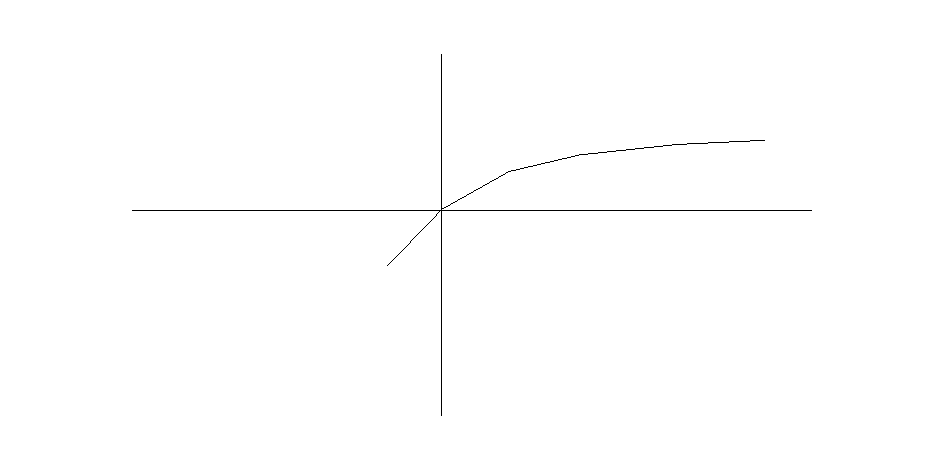
\includegraphics[width=0.8\textwidth]{img/herbrand}
        \caption{Herbrand Function}
    \end{figure}

\end{definition}

\begin{definition}
    The upper numbering of ramification groups is defined by:

    \[
        G(L / K)^{(t)} \coloneqq G(L / K)_{\eta_{L / K}^{-1} (t)}
    \]

    We call \(t\in [-1,\infty)\) a \underline{break} of upper ramification filtration if \(G(L / K)^{(t)} \supsetneq G(L / K)^{(t+\epsilon)}\) for all \(\epsilon > 0\).
\end{definition}

\begin{proposition}
    The breaks of the upper ramification filtration of \(G(L_m / K)\) are the non-negative integers:

    \[
        G(L_m / K)^{(n)} \underset{\phi}{\cong} U^{(n)} / U^{(m)}\, \text{ for } n = 0, \cdots ,m-1
    \]

    In particular: \(G(L_\pi / K)^{(n)} = \lim_{\leftarrow_m} G(L_m / K)^{(n)} \cong \lim_{\leftarrow_m} U^{(n)} / U^{(m)} \overset{\cong}{\leftarrow} U^{(n)} = 1 + (\pi^n)\)

\end{proposition}

Upper ramification numbering: If \(L \supset L^{\prime} \supset K\) are Galois extensions of \(K\), then \(\forall t \geq 1\):

\begin{center}
    \begin{tikzcd}
        & & G(L / K)^{(t)} \ar[r, two heads] \ar[d, hook] & G(L^\prime / K)^{(t)} \ar[d,hook] \\
        1 \ar[r] & G(L / L^\prime) \ar[r] & G(L / K) \ar[r, two heads] & G(L^\prime / K)
    \end{tikzcd}
\end{center}

Equivalently, \(G(L / K)^{(t)} G(L / L^{\prime}) / G(L / L^{\prime}) \cong G(L^{\prime} / K)^{(t)}\).

\begin{lemma}
    Let \(M / K\) be an abelian and purely ramified extension of \(K\) but not necessarily finite. Then the maximal unramified extnesion of \(M\) is \(M.K^{nr}\).   
\end{lemma}

\begin{proof}
    It is an immediate consequence of 10.6.
\end{proof}

\begin{lemma}
    If \(L / K\) is a purely ramified abelian extension, then the breaks of the upper ramification numbering are integers, and

    \[
        \forall n \geq -1: \left\vert G(L / K)^{(n)} / G(L / K)^{(n+1)} \right\vert \leq q
    \]

\end{lemma}

\begin{proof}
    Hasse-Arf theorem.
\end{proof}

\begin{proposition}
    Suppose \(L / K\) is abelian, \(L_\pi \subset L\) and \(L / L_\pi\) is purely ramified.

    Then, \(L = L_\pi\).
\end{proposition}

\begin{proof}
    Set \(G = G(L / K), H = \operatorname{Gal} (L / L_\pi)\) [which we want to prove is trivial].

    \underline{Claim (easy)}: The upper ramification filtration:
    
    \[
        \bigcap_{t\geq -1}^{} G^{(t)} = \{ 1 \} 
    \]

    Then we take \(n \geq 0\). Then, 
    
    \[
        \underbrace{[G^n : G^{n+1}]}_{12.13 \implies \leq q} = \underbrace{[(G / H)^n : (G / H)^{n+1}]}_{\geq q-1, = q \text{ when } n > 0}[G^n \cap H : G^{n+1} \cap H]
    \].

    So, if \(n \geq 1\) we must have \(G^n \cap H = G^{n+1} \cap H\). But \(G^0 = G \supset H\).

    In the case \(q \neq 2\) we have it for \(n \geq 0\).

    By induction we have \(H \subset G^n\) for all \(n \geq 0\).

    Then \(H \subset \bigcap_{n\geq -1} G^{(n)} = \{ 1 \} \) so \(H\) is trivial and thus \(L = L_\pi\).  
    
\end{proof}

From 12.14 one can deduce a proof of 12.9.

Tate: \(p\)-divisible groups.

\[
    T(G) = \lim_{\leftarrow} G[n](K^{\text{alg}}) \curvearrowleft \mathscr{G}_K = \operatorname{Gal} (K^{\text{alg}} / K)
\]

Suppose \(\zeta^p=1\).

\begin{center}
    \begin{tikzcd}
        \lim_{\leftarrow} \mu_{p^n}(\overline{\mathbb{Q}}_p) \ar[r,phantom,sloped,"\cong"] & \mathbb{Z}_p \ar[r,phantom,"\curvearrowleft"] & \mathscr{G}_{\mathbb{Q}_p} \\
        \mathbb{Z}_p(1) \ar[u,phantom,"\coloneqq"] & \chi_{\text{cyc}}(\sigma) \ar[u,phantom,sloped,"\in\mathbb{Z}_p^\times"] & \sigma \ar[u,phantom,sloped,"\in"] \ar[l,mapsto]
    \end{tikzcd}
\end{center}

Where:

\begin{center}
    \begin{tikzcd}
        \chi_{\text{cyc}}: & \mathscr{G}_{\mathbb{Q}} \ar[r] & \mathbb{Z}_p^\times \\ & \sigma \ar[r,mapsto] & u & \forall\zeta\in\mu_{p^\infty}:\sigma(\zeta)=\zeta^u=\zeta^{u\mod p^n}
    \end{tikzcd}
\end{center}

\end{document}